\documentclass[11pt, a4paper, USenglish]{article} % change ``USenglish'' to ``norsk'' if applicable.

\usepackage{kyblab} % Contains all included packages. See kyblab.sty.
\usepackage{float} % [H]
\renewcommand{\vec}[1]{\mathbf{#1}}
%matlab2tikz
\usepackage{pgfplots}
        \pgfplotsset{compat=newest}
        \pgfplotsset{plot coordinates/math parser=false}
\usepackage{tikz}
\usetikzlibrary{plotmarks}
  \usetikzlibrary{arrows.meta}
\usetikzlibrary{shapes.multipart}
\usepgfplotslibrary{patchplots}
\usepackage{grffile}
\newlength{\figureheight}
\newlength{\figurewidth}
%end matlab2tikz

\begin{document}
\subsection{Optimal Control of Pitch/Travel without Feedback}
\begin{figure}[H]
    \centering
    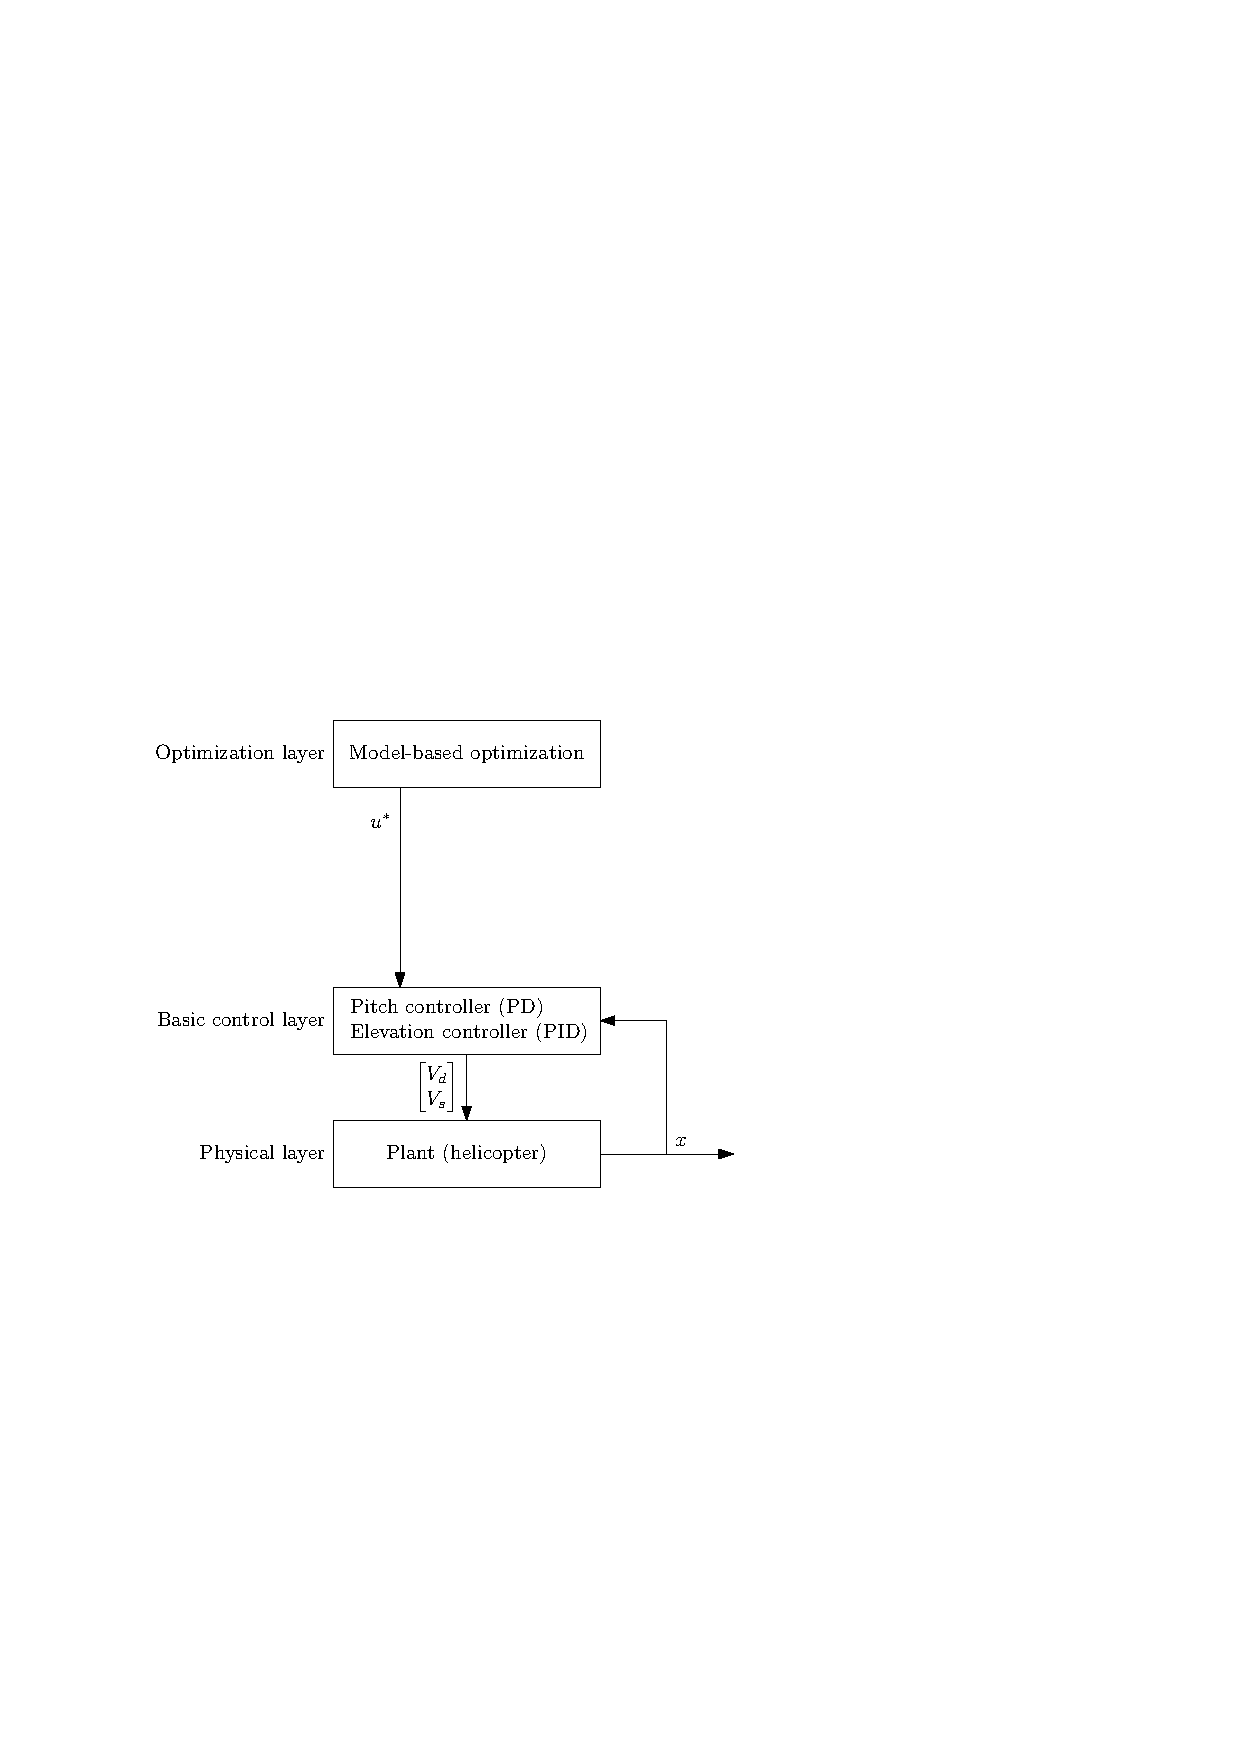
\includegraphics[width=1.00\textwidth]{figures/layers_openloop.pdf}
    \caption{A figure created with Ipe for TTK4135.}
\label{fig:layers_openloop}
\end{figure}

\begin{equation}
    \vec{\dot{x}} = A_c\vec{x} + B_c \vec{u} 
\end{equation}

\begin{equation*}
A_c =
    \begin{bmatrix}
        0 &  1 &  0 & 0 \\
        0 &  0 &  -K_2 & 0  \\
        0 &  0 &  0 & 1 \\
        0 &  0 & -K_1K_{pp} & -K_1K_{pd}                                 
    \end{bmatrix}
    , \quad B_c = 
    \begin{bmatrix} 0 \\ 0 \\ 0 \\ K_1K_{pp} \end{bmatrix}
\end{equation*}

\begin{align*}
    \vec{x_{k+1}} &= \vec{x_k} + h\vec{\dot{x}_k} \\
                  &= \vec{x_k} + h(A_c\vec{x_k} + B_c \vec{u_k}) \\  
                  &= (I + hA_C)\vec{x_k} + hB_c \vec{u_k} \\  
\end{align*}


\begin{figure}[H] 
        \centering
        \setlength{\figureheight}{6cm}
        \setlength{\figurewidth}{10cm}
        % This file was created by matlab2tikz.
%
%The latest updates can be retrieved from
%  http://www.mathworks.com/matlabcentral/fileexchange/22022-matlab2tikz-matlab2tikz
%where you can also make suggestions and rate matlab2tikz.
%
\begin{tikzpicture}

\begin{axis}[%
width=0.951\figurewidth,
height=\figureheight,
at={(0\figurewidth,0\figureheight)},
scale only axis,
separate axis lines,
every outer x axis line/.append style={black},
every x tick label/.append style={font=\color{black}},
xmin=0,
xmax=18,
xlabel={Time [s]},
every outer y axis line/.append style={black},
every y tick label/.append style={font=\color{black}},
ymin=-120,
ymax=40,
ylabel={$\lambda\text{ [deg]}$},
xmajorgrids,
ymajorgrids,
axis background/.style={fill=white}
]
\addplot [color=blue,solid,forget plot]
  table[row sep=crcr]{%
0	0\\
0.002	0\\
0.004	0\\
0.006	0\\
0.008	0\\
0.01	0\\
0.012	0\\
0.014	0\\
0.016	0\\
0.018	0\\
0.02	0\\
0.022	0\\
0.024	0\\
0.026	0\\
0.028	0\\
0.03	0\\
0.032	0\\
0.034	0\\
0.036	0\\
0.038	0\\
0.04	0\\
0.042	0\\
0.044	0\\
0.046	0\\
0.048	0\\
0.05	0\\
0.052	0\\
0.054	0\\
0.056	0\\
0.058	0\\
0.06	0\\
0.062	0\\
0.064	0\\
0.066	0\\
0.068	0\\
0.07	0\\
0.072	0\\
0.074	0\\
0.076	0\\
0.078	0\\
0.08	0\\
0.082	0\\
0.084	0\\
0.086	0.0439453125\\
0.088	0.0439453125\\
0.09	0.0439453125\\
0.092	0.0439453125\\
0.094	0.0439453125\\
0.096	0.0439453125\\
0.098	0.0439453125\\
0.1	0.0439453125\\
0.102	0.0439453125\\
0.104	0.0439453125\\
0.106	0.0439453125\\
0.108	0.0439453125\\
0.11	0.0439453125\\
0.112	0.0439453125\\
0.114	0.0439453125\\
0.116	0.0439453125\\
0.118	0.0439453125\\
0.12	0.0439453125\\
0.122	0.0439453125\\
0.124	0.0439453125\\
0.126	0.087890625\\
0.128	0.087890625\\
0.13	0.087890625\\
0.132	0.087890625\\
0.134	0.087890625\\
0.136	0.087890625\\
0.138	0.087890625\\
0.14	0.087890625\\
0.142	0.087890625\\
0.144	0.087890625\\
0.146	0.087890625\\
0.148	0.087890625\\
0.15	0.087890625\\
0.152	0.087890625\\
0.154	0.1318359375\\
0.156	0.1318359375\\
0.158	0.1318359375\\
0.16	0.1318359375\\
0.162	0.1318359375\\
0.164	0.1318359375\\
0.166	0.1318359375\\
0.168	0.1318359375\\
0.17	0.1318359375\\
0.172	0.1318359375\\
0.174	0.1318359375\\
0.176	0.17578125\\
0.178	0.17578125\\
0.18	0.17578125\\
0.182	0.17578125\\
0.184	0.17578125\\
0.186	0.2197265625\\
0.188	0.2197265625\\
0.19	0.2197265625\\
0.192	0.2197265625\\
0.194	0.17578125\\
0.196	0.17578125\\
0.198	0.2197265625\\
0.2	0.2197265625\\
0.202	0.2197265625\\
0.204	0.2197265625\\
0.206	0.2197265625\\
0.208	0.263671875\\
0.21	0.263671875\\
0.212	0.263671875\\
0.214	0.263671875\\
0.216	0.263671875\\
0.218	0.263671875\\
0.22	0.263671875\\
0.222	0.263671875\\
0.224	0.263671875\\
0.226	0.263671875\\
0.228	0.263671875\\
0.23	0.3076171875\\
0.232	0.3076171875\\
0.234	0.3076171875\\
0.236	0.3076171875\\
0.238	0.3076171875\\
0.24	0.3515625\\
0.242	0.3515625\\
0.244	0.3515625\\
0.246	0.3515625\\
0.248	0.3515625\\
0.25	0.3515625\\
0.252	0.3515625\\
0.254	0.3515625\\
0.256	0.3515625\\
0.258	0.3955078125\\
0.26	0.3955078125\\
0.262	0.3955078125\\
0.264	0.3955078125\\
0.266	0.3955078125\\
0.268	0.3955078125\\
0.27	0.3955078125\\
0.272	0.439453125\\
0.274	0.439453125\\
0.276	0.439453125\\
0.278	0.439453125\\
0.28	0.439453125\\
0.282	0.439453125\\
0.284	0.439453125\\
0.286	0.439453125\\
0.288	0.4833984375\\
0.29	0.4833984375\\
0.292	0.4833984375\\
0.294	0.4833984375\\
0.296	0.4833984375\\
0.298	0.4833984375\\
0.3	0.4833984375\\
0.302	0.52734375\\
0.304	0.52734375\\
0.306	0.52734375\\
0.308	0.52734375\\
0.31	0.52734375\\
0.312	0.52734375\\
0.314	0.52734375\\
0.316	0.5712890625\\
0.318	0.5712890625\\
0.32	0.5712890625\\
0.322	0.5712890625\\
0.324	0.5712890625\\
0.326	0.5712890625\\
0.328	0.5712890625\\
0.33	0.5712890625\\
0.332	0.615234375\\
0.334	0.6591796875\\
0.336	0.6591796875\\
0.338	0.6591796875\\
0.34	0.615234375\\
0.342	0.615234375\\
0.344	0.6591796875\\
0.346	0.6591796875\\
0.348	0.703125\\
0.35	0.703125\\
0.352	0.703125\\
0.354	0.6591796875\\
0.356	0.6591796875\\
0.358	0.6591796875\\
0.36	0.703125\\
0.362	0.7470703125\\
0.364	0.7470703125\\
0.366	0.7470703125\\
0.368	0.7470703125\\
0.37	0.7470703125\\
0.372	0.7470703125\\
0.374	0.7470703125\\
0.376	0.791015625\\
0.378	0.791015625\\
0.38	0.791015625\\
0.382	0.791015625\\
0.384	0.791015625\\
0.386	0.791015625\\
0.388	0.791015625\\
0.39	0.8349609375\\
0.392	0.8349609375\\
0.394	0.87890625\\
0.396	0.8349609375\\
0.398	0.8349609375\\
0.4	0.8349609375\\
0.402	0.8349609375\\
0.404	0.87890625\\
0.406	0.87890625\\
0.408	0.9228515625\\
0.41	0.9228515625\\
0.412	0.87890625\\
0.414	0.87890625\\
0.416	0.87890625\\
0.418	0.9228515625\\
0.42	0.966796875\\
0.422	0.966796875\\
0.424	0.966796875\\
0.426	0.9228515625\\
0.428	0.9228515625\\
0.43	0.9228515625\\
0.432	0.966796875\\
0.434	1.0107421875\\
0.436	1.0107421875\\
0.438	1.0107421875\\
0.44	1.0107421875\\
0.442	1.0107421875\\
0.444	0.966796875\\
0.446	1.0107421875\\
0.448	1.0546875\\
0.45	1.0546875\\
0.452	1.0546875\\
0.454	1.0546875\\
0.456	1.0546875\\
0.458	1.0546875\\
0.46	1.0546875\\
0.462	1.0986328125\\
0.464	1.0986328125\\
0.466	1.142578125\\
0.468	1.142578125\\
0.47	1.0986328125\\
0.472	1.0986328125\\
0.474	1.0986328125\\
0.476	1.142578125\\
0.478	1.142578125\\
0.48	1.1865234375\\
0.482	1.1865234375\\
0.484	1.142578125\\
0.486	1.142578125\\
0.488	1.142578125\\
0.49	1.1865234375\\
0.492	1.1865234375\\
0.494	1.23046875\\
0.496	1.23046875\\
0.498	1.23046875\\
0.5	1.23046875\\
0.502	1.23046875\\
0.504	1.23046875\\
0.506	1.23046875\\
0.508	1.2744140625\\
0.51	1.2744140625\\
0.512	1.2744140625\\
0.514	1.2744140625\\
0.516	1.2744140625\\
0.518	1.2744140625\\
0.52	1.318359375\\
0.522	1.318359375\\
0.524	1.318359375\\
0.526	1.318359375\\
0.528	1.318359375\\
0.53	1.318359375\\
0.532	1.318359375\\
0.534	1.3623046875\\
0.536	1.3623046875\\
0.538	1.3623046875\\
0.54	1.3623046875\\
0.542	1.3623046875\\
0.544	1.40625\\
0.546	1.40625\\
0.548	1.40625\\
0.55	1.40625\\
0.552	1.40625\\
0.554	1.40625\\
0.556	1.4501953125\\
0.558	1.4501953125\\
0.56	1.4501953125\\
0.562	1.4501953125\\
0.564	1.4501953125\\
0.566	1.4501953125\\
0.568	1.4501953125\\
0.57	1.494140625\\
0.572	1.494140625\\
0.574	1.494140625\\
0.576	1.494140625\\
0.578	1.494140625\\
0.58	1.494140625\\
0.582	1.494140625\\
0.584	1.5380859375\\
0.586	1.5380859375\\
0.588	1.5380859375\\
0.59	1.5380859375\\
0.592	1.58203125\\
0.594	1.58203125\\
0.596	1.58203125\\
0.598	1.58203125\\
0.6	1.58203125\\
0.602	1.58203125\\
0.604	1.6259765625\\
0.606	1.6259765625\\
0.608	1.6259765625\\
0.61	1.6259765625\\
0.612	1.6259765625\\
0.614	1.6259765625\\
0.616	1.6259765625\\
0.618	1.669921875\\
0.62	1.669921875\\
0.622	1.669921875\\
0.624	1.669921875\\
0.626	1.669921875\\
0.628	1.669921875\\
0.63	1.7138671875\\
0.632	1.7138671875\\
0.634	1.7138671875\\
0.636	1.7138671875\\
0.638	1.7138671875\\
0.64	1.7138671875\\
0.642	1.7578125\\
0.644	1.7578125\\
0.646	1.7578125\\
0.648	1.7578125\\
0.65	1.7578125\\
0.652	1.7578125\\
0.654	1.8017578125\\
0.656	1.8017578125\\
0.658	1.8017578125\\
0.66	1.8017578125\\
0.662	1.8017578125\\
0.664	1.8017578125\\
0.666	1.8017578125\\
0.668	1.845703125\\
0.67	1.845703125\\
0.672	1.845703125\\
0.674	1.845703125\\
0.676	1.845703125\\
0.678	1.845703125\\
0.68	1.845703125\\
0.682	1.845703125\\
0.684	1.8896484375\\
0.686	1.8896484375\\
0.688	1.8896484375\\
0.69	1.8896484375\\
0.692	1.93359375\\
0.694	1.93359375\\
0.696	1.93359375\\
0.698	1.93359375\\
0.7	1.93359375\\
0.702	1.93359375\\
0.704	1.93359375\\
0.706	1.93359375\\
0.708	1.9775390625\\
0.71	1.9775390625\\
0.712	1.9775390625\\
0.714	1.9775390625\\
0.716	1.9775390625\\
0.718	1.9775390625\\
0.72	1.9775390625\\
0.722	2.021484375\\
0.724	2.021484375\\
0.726	2.021484375\\
0.728	2.021484375\\
0.73	2.021484375\\
0.732	2.021484375\\
0.734	2.021484375\\
0.736	2.021484375\\
0.738	2.0654296875\\
0.74	2.0654296875\\
0.742	2.0654296875\\
0.744	2.0654296875\\
0.746	2.0654296875\\
0.748	2.0654296875\\
0.75	2.109375\\
0.752	2.109375\\
0.754	2.109375\\
0.756	2.109375\\
0.758	2.109375\\
0.76	2.109375\\
0.762	2.109375\\
0.764	2.1533203125\\
0.766	2.1533203125\\
0.768	2.1533203125\\
0.77	2.1533203125\\
0.772	2.1533203125\\
0.774	2.1533203125\\
0.776	2.1533203125\\
0.778	2.1533203125\\
0.78	2.197265625\\
0.782	2.197265625\\
0.784	2.197265625\\
0.786	2.197265625\\
0.788	2.197265625\\
0.79	2.2412109375\\
0.792	2.2412109375\\
0.794	2.2412109375\\
0.796	2.2412109375\\
0.798	2.2412109375\\
0.8	2.2412109375\\
0.802	2.2412109375\\
0.804	2.2412109375\\
0.806	2.28515625\\
0.808	2.28515625\\
0.81	2.28515625\\
0.812	2.28515625\\
0.814	2.28515625\\
0.816	2.28515625\\
0.818	2.28515625\\
0.82	2.28515625\\
0.822	2.3291015625\\
0.824	2.3291015625\\
0.826	2.3291015625\\
0.828	2.3291015625\\
0.83	2.3291015625\\
0.832	2.3291015625\\
0.834	2.3291015625\\
0.836	2.3291015625\\
0.838	2.373046875\\
0.84	2.373046875\\
0.842	2.373046875\\
0.844	2.373046875\\
0.846	2.373046875\\
0.848	2.373046875\\
0.85	2.4169921875\\
0.852	2.4169921875\\
0.854	2.4169921875\\
0.856	2.4169921875\\
0.858	2.4169921875\\
0.86	2.4169921875\\
0.862	2.4169921875\\
0.864	2.4169921875\\
0.866	2.4169921875\\
0.868	2.4609375\\
0.87	2.4609375\\
0.872	2.4609375\\
0.874	2.4609375\\
0.876	2.4609375\\
0.878	2.4609375\\
0.88	2.4609375\\
0.882	2.5048828125\\
0.884	2.5048828125\\
0.886	2.5048828125\\
0.888	2.5048828125\\
0.89	2.5048828125\\
0.892	2.5048828125\\
0.894	2.5048828125\\
0.896	2.548828125\\
0.898	2.548828125\\
0.9	2.548828125\\
0.902	2.548828125\\
0.904	2.548828125\\
0.906	2.548828125\\
0.908	2.548828125\\
0.91	2.548828125\\
0.912	2.5927734375\\
0.914	2.5927734375\\
0.916	2.5927734375\\
0.918	2.5927734375\\
0.92	2.5927734375\\
0.922	2.5927734375\\
0.924	2.5927734375\\
0.926	2.5927734375\\
0.928	2.5927734375\\
0.93	2.63671875\\
0.932	2.63671875\\
0.934	2.63671875\\
0.936	2.63671875\\
0.938	2.63671875\\
0.94	2.63671875\\
0.942	2.6806640625\\
0.944	2.6806640625\\
0.946	2.6806640625\\
0.948	2.6806640625\\
0.95	2.6806640625\\
0.952	2.6806640625\\
0.954	2.6806640625\\
0.956	2.6806640625\\
0.958	2.6806640625\\
0.96	2.724609375\\
0.962	2.724609375\\
0.964	2.724609375\\
0.966	2.724609375\\
0.968	2.724609375\\
0.97	2.724609375\\
0.972	2.724609375\\
0.974	2.724609375\\
0.976	2.724609375\\
0.978	2.7685546875\\
0.98	2.7685546875\\
0.982	2.7685546875\\
0.984	2.7685546875\\
0.986	2.7685546875\\
0.988	2.8125\\
0.99	2.8125\\
0.992	2.8125\\
0.994	2.8125\\
0.996	2.8125\\
0.998	2.8125\\
1	2.8125\\
1.002	2.8125\\
1.004	2.8125\\
1.006	2.8125\\
1.008	2.8125\\
1.01	2.8564453125\\
1.012	2.8564453125\\
1.014	2.8564453125\\
1.016	2.8564453125\\
1.018	2.8564453125\\
1.02	2.8564453125\\
1.022	2.8564453125\\
1.024	2.8564453125\\
1.026	2.8564453125\\
1.028	2.900390625\\
1.03	2.900390625\\
1.032	2.900390625\\
1.034	2.900390625\\
1.036	2.900390625\\
1.038	2.900390625\\
1.04	2.9443359375\\
1.042	2.9443359375\\
1.044	2.9443359375\\
1.046	2.9443359375\\
1.048	2.9443359375\\
1.05	2.9443359375\\
1.052	2.9443359375\\
1.054	2.9443359375\\
1.056	2.9443359375\\
1.058	2.9443359375\\
1.06	2.98828125\\
1.062	2.98828125\\
1.064	2.98828125\\
1.066	2.98828125\\
1.068	2.98828125\\
1.07	2.98828125\\
1.072	2.98828125\\
1.074	2.98828125\\
1.076	2.98828125\\
1.078	3.0322265625\\
1.08	3.0322265625\\
1.082	3.0322265625\\
1.084	3.0322265625\\
1.086	3.0322265625\\
1.088	3.0322265625\\
1.09	3.0322265625\\
1.092	3.076171875\\
1.094	3.076171875\\
1.096	3.076171875\\
1.098	3.076171875\\
1.1	3.076171875\\
1.102	3.076171875\\
1.104	3.076171875\\
1.106	3.076171875\\
1.108	3.076171875\\
1.11	3.076171875\\
1.112	3.1201171875\\
1.114	3.1201171875\\
1.116	3.1201171875\\
1.118	3.1201171875\\
1.12	3.1201171875\\
1.122	3.1201171875\\
1.124	3.1201171875\\
1.126	3.1201171875\\
1.128	3.1201171875\\
1.13	3.1201171875\\
1.132	3.1640625\\
1.134	3.1640625\\
1.136	3.1640625\\
1.138	3.1640625\\
1.14	3.1640625\\
1.142	3.1640625\\
1.144	3.2080078125\\
1.146	3.2080078125\\
1.148	3.2080078125\\
1.15	3.2080078125\\
1.152	3.2080078125\\
1.154	3.2080078125\\
1.156	3.2080078125\\
1.158	3.2080078125\\
1.16	3.2080078125\\
1.162	3.2080078125\\
1.164	3.2080078125\\
1.166	3.251953125\\
1.168	3.251953125\\
1.17	3.251953125\\
1.172	3.251953125\\
1.174	3.251953125\\
1.176	3.251953125\\
1.178	3.251953125\\
1.18	3.251953125\\
1.182	3.251953125\\
1.184	3.251953125\\
1.186	3.251953125\\
1.188	3.2958984375\\
1.19	3.2958984375\\
1.192	3.2958984375\\
1.194	3.2958984375\\
1.196	3.33984375\\
1.198	3.33984375\\
1.2	3.33984375\\
1.202	3.33984375\\
1.204	3.33984375\\
1.206	3.33984375\\
1.208	3.33984375\\
1.21	3.33984375\\
1.212	3.33984375\\
1.214	3.33984375\\
1.216	3.33984375\\
1.218	3.3837890625\\
1.22	3.3837890625\\
1.222	3.3837890625\\
1.224	3.3837890625\\
1.226	3.3837890625\\
1.228	3.3837890625\\
1.23	3.3837890625\\
1.232	3.3837890625\\
1.234	3.3837890625\\
1.236	3.3837890625\\
1.238	3.3837890625\\
1.24	3.427734375\\
1.242	3.427734375\\
1.244	3.427734375\\
1.246	3.427734375\\
1.248	3.427734375\\
1.25	3.427734375\\
1.252	3.427734375\\
1.254	3.427734375\\
1.256	3.4716796875\\
1.258	3.4716796875\\
1.26	3.4716796875\\
1.262	3.4716796875\\
1.264	3.4716796875\\
1.266	3.4716796875\\
1.268	3.4716796875\\
1.27	3.4716796875\\
1.272	3.515625\\
1.274	3.515625\\
1.276	3.515625\\
1.278	3.515625\\
1.28	3.515625\\
1.282	3.515625\\
1.284	3.515625\\
1.286	3.515625\\
1.288	3.515625\\
1.29	3.515625\\
1.292	3.5595703125\\
1.294	3.5595703125\\
1.296	3.5595703125\\
1.298	3.5595703125\\
1.3	3.5595703125\\
1.302	3.5595703125\\
1.304	3.5595703125\\
1.306	3.5595703125\\
1.308	3.5595703125\\
1.31	3.603515625\\
1.312	3.603515625\\
1.314	3.603515625\\
1.316	3.603515625\\
1.318	3.603515625\\
1.32	3.603515625\\
1.322	3.603515625\\
1.324	3.603515625\\
1.326	3.603515625\\
1.328	3.6474609375\\
1.33	3.6474609375\\
1.332	3.6474609375\\
1.334	3.6474609375\\
1.336	3.6474609375\\
1.338	3.6474609375\\
1.34	3.6474609375\\
1.342	3.6474609375\\
1.344	3.6474609375\\
1.346	3.69140625\\
1.348	3.69140625\\
1.35	3.69140625\\
1.352	3.69140625\\
1.354	3.69140625\\
1.356	3.69140625\\
1.358	3.69140625\\
1.36	3.69140625\\
1.362	3.7353515625\\
1.364	3.7353515625\\
1.366	3.7353515625\\
1.368	3.7353515625\\
1.37	3.7353515625\\
1.372	3.7353515625\\
1.374	3.7353515625\\
1.376	3.7353515625\\
1.378	3.7353515625\\
1.38	3.7353515625\\
1.382	3.779296875\\
1.384	3.779296875\\
1.386	3.779296875\\
1.388	3.779296875\\
1.39	3.779296875\\
1.392	3.779296875\\
1.394	3.779296875\\
1.396	3.779296875\\
1.398	3.779296875\\
1.4	3.779296875\\
1.402	3.779296875\\
1.404	3.8232421875\\
1.406	3.8232421875\\
1.408	3.8232421875\\
1.41	3.8232421875\\
1.412	3.8232421875\\
1.414	3.8232421875\\
1.416	3.8671875\\
1.418	3.8671875\\
1.42	3.8671875\\
1.422	3.8671875\\
1.424	3.8671875\\
1.426	3.8671875\\
1.428	3.8671875\\
1.43	3.8671875\\
1.432	3.8671875\\
1.434	3.9111328125\\
1.436	3.9111328125\\
1.438	3.9111328125\\
1.44	3.9111328125\\
1.442	3.9111328125\\
1.444	3.9111328125\\
1.446	3.9111328125\\
1.448	3.9111328125\\
1.45	3.9111328125\\
1.452	3.9111328125\\
1.454	3.9111328125\\
1.456	3.955078125\\
1.458	3.955078125\\
1.46	3.955078125\\
1.462	3.955078125\\
1.464	3.955078125\\
1.466	3.955078125\\
1.468	3.955078125\\
1.47	3.955078125\\
1.472	3.955078125\\
1.474	3.955078125\\
1.476	3.9990234375\\
1.478	3.9990234375\\
1.48	3.9990234375\\
1.482	3.9990234375\\
1.484	3.9990234375\\
1.486	4.04296875\\
1.488	4.04296875\\
1.49	4.04296875\\
1.492	4.04296875\\
1.494	4.04296875\\
1.496	4.04296875\\
1.498	4.04296875\\
1.5	4.04296875\\
1.502	4.04296875\\
1.504	4.04296875\\
1.506	4.04296875\\
1.508	4.0869140625\\
1.51	4.0869140625\\
1.512	4.0869140625\\
1.514	4.0869140625\\
1.516	4.0869140625\\
1.518	4.0869140625\\
1.52	4.0869140625\\
1.522	4.0869140625\\
1.524	4.0869140625\\
1.526	4.0869140625\\
1.528	4.0869140625\\
1.53	4.130859375\\
1.532	4.130859375\\
1.534	4.130859375\\
1.536	4.130859375\\
1.538	4.1748046875\\
1.54	4.1748046875\\
1.542	4.1748046875\\
1.544	4.1748046875\\
1.546	4.1748046875\\
1.548	4.1748046875\\
1.55	4.1748046875\\
1.552	4.1748046875\\
1.554	4.1748046875\\
1.556	4.1748046875\\
1.558	4.1748046875\\
1.56	4.21875\\
1.562	4.21875\\
1.564	4.21875\\
1.566	4.21875\\
1.568	4.21875\\
1.57	4.21875\\
1.572	4.21875\\
1.574	4.21875\\
1.576	4.21875\\
1.578	4.21875\\
1.58	4.2626953125\\
1.582	4.2626953125\\
1.584	4.2626953125\\
1.586	4.2626953125\\
1.588	4.2626953125\\
1.59	4.2626953125\\
1.592	4.306640625\\
1.594	4.306640625\\
1.596	4.306640625\\
1.598	4.306640625\\
1.6	4.306640625\\
1.602	4.306640625\\
1.604	4.306640625\\
1.606	4.306640625\\
1.608	4.306640625\\
1.61	4.306640625\\
1.612	4.3505859375\\
1.614	4.3505859375\\
1.616	4.3505859375\\
1.618	4.3505859375\\
1.62	4.3505859375\\
1.622	4.3505859375\\
1.624	4.3505859375\\
1.626	4.3505859375\\
1.628	4.3505859375\\
1.63	4.39453125\\
1.632	4.39453125\\
1.634	4.39453125\\
1.636	4.39453125\\
1.638	4.39453125\\
1.64	4.39453125\\
1.642	4.39453125\\
1.644	4.39453125\\
1.646	4.39453125\\
1.648	4.39453125\\
1.65	4.39453125\\
1.652	4.4384765625\\
1.654	4.4384765625\\
1.656	4.4384765625\\
1.658	4.4384765625\\
1.66	4.4384765625\\
1.662	4.4384765625\\
1.664	4.482421875\\
1.666	4.482421875\\
1.668	4.482421875\\
1.67	4.482421875\\
1.672	4.482421875\\
1.674	4.482421875\\
1.676	4.482421875\\
1.678	4.482421875\\
1.68	4.482421875\\
1.682	4.5263671875\\
1.684	4.5263671875\\
1.686	4.5263671875\\
1.688	4.5263671875\\
1.69	4.5263671875\\
1.692	4.5263671875\\
1.694	4.5263671875\\
1.696	4.5263671875\\
1.698	4.5703125\\
1.7	4.5703125\\
1.702	4.5703125\\
1.704	4.5703125\\
1.706	4.5703125\\
1.708	4.5703125\\
1.71	4.5703125\\
1.712	4.5703125\\
1.714	4.5703125\\
1.716	4.5703125\\
1.718	4.6142578125\\
1.72	4.6142578125\\
1.722	4.6142578125\\
1.724	4.6142578125\\
1.726	4.6142578125\\
1.728	4.6142578125\\
1.73	4.6142578125\\
1.732	4.658203125\\
1.734	4.658203125\\
1.736	4.658203125\\
1.738	4.658203125\\
1.74	4.658203125\\
1.742	4.658203125\\
1.744	4.658203125\\
1.746	4.658203125\\
1.748	4.7021484375\\
1.75	4.7021484375\\
1.752	4.7021484375\\
1.754	4.7021484375\\
1.756	4.7021484375\\
1.758	4.7021484375\\
1.76	4.7021484375\\
1.762	4.7021484375\\
1.764	4.7021484375\\
1.766	4.74609375\\
1.768	4.74609375\\
1.77	4.74609375\\
1.772	4.74609375\\
1.774	4.74609375\\
1.776	4.74609375\\
1.778	4.74609375\\
1.78	4.74609375\\
1.782	4.74609375\\
1.784	4.7900390625\\
1.786	4.7900390625\\
1.788	4.7900390625\\
1.79	4.7900390625\\
1.792	4.7900390625\\
1.794	4.7900390625\\
1.796	4.7900390625\\
1.798	4.833984375\\
1.8	4.833984375\\
1.802	4.833984375\\
1.804	4.833984375\\
1.806	4.833984375\\
1.808	4.833984375\\
1.81	4.833984375\\
1.812	4.833984375\\
1.814	4.833984375\\
1.816	4.8779296875\\
1.818	4.8779296875\\
1.82	4.8779296875\\
1.822	4.8779296875\\
1.824	4.8779296875\\
1.826	4.8779296875\\
1.828	4.8779296875\\
1.83	4.921875\\
1.832	4.921875\\
1.834	4.921875\\
1.836	4.921875\\
1.838	4.921875\\
1.84	4.921875\\
1.842	4.921875\\
1.844	4.921875\\
1.846	4.9658203125\\
1.848	4.9658203125\\
1.85	4.9658203125\\
1.852	4.9658203125\\
1.854	4.9658203125\\
1.856	4.9658203125\\
1.858	4.9658203125\\
1.86	4.9658203125\\
1.862	5.009765625\\
1.864	5.009765625\\
1.866	5.009765625\\
1.868	5.009765625\\
1.87	5.009765625\\
1.872	5.009765625\\
1.874	5.009765625\\
1.876	5.0537109375\\
1.878	5.0537109375\\
1.88	5.0537109375\\
1.882	5.0537109375\\
1.884	5.0537109375\\
1.886	5.0537109375\\
1.888	5.0537109375\\
1.89	5.0537109375\\
1.892	5.0537109375\\
1.894	5.09765625\\
1.896	5.09765625\\
1.898	5.09765625\\
1.9	5.09765625\\
1.902	5.09765625\\
1.904	5.09765625\\
1.906	5.09765625\\
1.908	5.09765625\\
1.91	5.09765625\\
1.912	5.1416015625\\
1.914	5.1416015625\\
1.916	5.1416015625\\
1.918	5.1416015625\\
1.92	5.1416015625\\
1.922	5.1416015625\\
1.924	5.185546875\\
1.926	5.185546875\\
1.928	5.185546875\\
1.93	5.185546875\\
1.932	5.185546875\\
1.934	5.185546875\\
1.936	5.185546875\\
1.938	5.185546875\\
1.94	5.2294921875\\
1.942	5.2294921875\\
1.944	5.2294921875\\
1.946	5.2294921875\\
1.948	5.2294921875\\
1.95	5.2294921875\\
1.952	5.2294921875\\
1.954	5.2294921875\\
1.956	5.2734375\\
1.958	5.2734375\\
1.96	5.2734375\\
1.962	5.2734375\\
1.964	5.2734375\\
1.966	5.2734375\\
1.968	5.3173828125\\
1.97	5.3173828125\\
1.972	5.3173828125\\
1.974	5.3173828125\\
1.976	5.3173828125\\
1.978	5.3173828125\\
1.98	5.3173828125\\
1.982	5.3173828125\\
1.984	5.3173828125\\
1.986	5.361328125\\
1.988	5.361328125\\
1.99	5.361328125\\
1.992	5.361328125\\
1.994	5.361328125\\
1.996	5.361328125\\
1.998	5.361328125\\
2	5.4052734375\\
2.002	5.4052734375\\
2.004	5.4052734375\\
2.006	5.4052734375\\
2.008	5.4052734375\\
2.01	5.4052734375\\
2.012	5.4052734375\\
2.014	5.4052734375\\
2.016	5.4052734375\\
2.018	5.44921875\\
2.02	5.44921875\\
2.022	5.44921875\\
2.024	5.44921875\\
2.026	5.44921875\\
2.028	5.44921875\\
2.03	5.4931640625\\
2.032	5.4931640625\\
2.034	5.4931640625\\
2.036	5.4931640625\\
2.038	5.4931640625\\
2.04	5.4931640625\\
2.042	5.4931640625\\
2.044	5.4931640625\\
2.046	5.4931640625\\
2.048	5.537109375\\
2.05	5.537109375\\
2.052	5.537109375\\
2.054	5.537109375\\
2.056	5.537109375\\
2.058	5.537109375\\
2.06	5.5810546875\\
2.062	5.5810546875\\
2.064	5.5810546875\\
2.066	5.5810546875\\
2.068	5.5810546875\\
2.07	5.5810546875\\
2.072	5.5810546875\\
2.074	5.625\\
2.076	5.625\\
2.078	5.625\\
2.08	5.625\\
2.082	5.625\\
2.084	5.625\\
2.086	5.625\\
2.088	5.625\\
2.09	5.6689453125\\
2.092	5.6689453125\\
2.094	5.6689453125\\
2.096	5.6689453125\\
2.098	5.6689453125\\
2.1	5.6689453125\\
2.102	5.6689453125\\
2.104	5.6689453125\\
2.106	5.712890625\\
2.108	5.712890625\\
2.11	5.712890625\\
2.112	5.712890625\\
2.114	5.712890625\\
2.116	5.712890625\\
2.118	5.712890625\\
2.12	5.7568359375\\
2.122	5.7568359375\\
2.124	5.7568359375\\
2.126	5.7568359375\\
2.128	5.7568359375\\
2.13	5.80078125\\
2.132	5.80078125\\
2.134	5.80078125\\
2.136	5.80078125\\
2.138	5.80078125\\
2.14	5.80078125\\
2.142	5.80078125\\
2.144	5.80078125\\
2.146	5.80078125\\
2.148	5.8447265625\\
2.15	5.8447265625\\
2.152	5.8447265625\\
2.154	5.8447265625\\
2.156	5.8447265625\\
2.158	5.8447265625\\
2.16	5.888671875\\
2.162	5.888671875\\
2.164	5.888671875\\
2.166	5.888671875\\
2.168	5.888671875\\
2.17	5.888671875\\
2.172	5.888671875\\
2.174	5.888671875\\
2.176	5.888671875\\
2.178	5.9326171875\\
2.18	5.9326171875\\
2.182	5.9326171875\\
2.184	5.9326171875\\
2.186	5.9326171875\\
2.188	5.9326171875\\
2.19	5.9765625\\
2.192	5.9765625\\
2.194	5.9765625\\
2.196	5.9765625\\
2.198	5.9765625\\
2.2	5.9765625\\
2.202	6.0205078125\\
2.204	6.0205078125\\
2.206	6.0205078125\\
2.208	6.0205078125\\
2.21	6.0205078125\\
2.212	6.0205078125\\
2.214	6.0205078125\\
2.216	6.064453125\\
2.218	6.064453125\\
2.22	6.064453125\\
2.222	6.064453125\\
2.224	6.064453125\\
2.226	6.064453125\\
2.228	6.064453125\\
2.23	6.1083984375\\
2.232	6.1083984375\\
2.234	6.1083984375\\
2.236	6.1083984375\\
2.238	6.1083984375\\
2.24	6.1083984375\\
2.242	6.15234375\\
2.244	6.15234375\\
2.246	6.15234375\\
2.248	6.15234375\\
2.25	6.15234375\\
2.252	6.15234375\\
2.254	6.15234375\\
2.256	6.15234375\\
2.258	6.1962890625\\
2.26	6.1962890625\\
2.262	6.1962890625\\
2.264	6.1962890625\\
2.266	6.1962890625\\
2.268	6.1962890625\\
2.27	6.240234375\\
2.272	6.240234375\\
2.274	6.240234375\\
2.276	6.240234375\\
2.278	6.240234375\\
2.28	6.240234375\\
2.282	6.2841796875\\
2.284	6.2841796875\\
2.286	6.2841796875\\
2.288	6.2841796875\\
2.29	6.2841796875\\
2.292	6.2841796875\\
2.294	6.2841796875\\
2.296	6.2841796875\\
2.298	6.328125\\
2.3	6.328125\\
2.302	6.328125\\
2.304	6.328125\\
2.306	6.328125\\
2.308	6.328125\\
2.31	6.3720703125\\
2.312	6.3720703125\\
2.314	6.3720703125\\
2.316	6.3720703125\\
2.318	6.3720703125\\
2.32	6.3720703125\\
2.322	6.416015625\\
2.324	6.416015625\\
2.326	6.416015625\\
2.328	6.416015625\\
2.33	6.416015625\\
2.332	6.416015625\\
2.334	6.416015625\\
2.336	6.416015625\\
2.338	6.4599609375\\
2.34	6.4599609375\\
2.342	6.4599609375\\
2.344	6.4599609375\\
2.346	6.4599609375\\
2.348	6.4599609375\\
2.35	6.50390625\\
2.352	6.50390625\\
2.354	6.50390625\\
2.356	6.50390625\\
2.358	6.50390625\\
2.36	6.50390625\\
2.362	6.5478515625\\
2.364	6.5478515625\\
2.366	6.5478515625\\
2.368	6.5478515625\\
2.37	6.5478515625\\
2.372	6.5478515625\\
2.374	6.5478515625\\
2.376	6.5478515625\\
2.378	6.591796875\\
2.38	6.591796875\\
2.382	6.591796875\\
2.384	6.591796875\\
2.386	6.591796875\\
2.388	6.6357421875\\
2.39	6.6357421875\\
2.392	6.6357421875\\
2.394	6.6357421875\\
2.396	6.6357421875\\
2.398	6.6357421875\\
2.4	6.6796875\\
2.402	6.6796875\\
2.404	6.6796875\\
2.406	6.6796875\\
2.408	6.6796875\\
2.41	6.6796875\\
2.412	6.6796875\\
2.414	6.7236328125\\
2.416	6.7236328125\\
2.418	6.7236328125\\
2.42	6.7236328125\\
2.422	6.7236328125\\
2.424	6.7236328125\\
2.426	6.767578125\\
2.428	6.767578125\\
2.43	6.767578125\\
2.432	6.767578125\\
2.434	6.767578125\\
2.436	6.767578125\\
2.438	6.8115234375\\
2.44	6.8115234375\\
2.442	6.8115234375\\
2.444	6.8115234375\\
2.446	6.8115234375\\
2.448	6.8115234375\\
2.45	6.85546875\\
2.452	6.85546875\\
2.454	6.85546875\\
2.456	6.85546875\\
2.458	6.85546875\\
2.46	6.85546875\\
2.462	6.85546875\\
2.464	6.8994140625\\
2.466	6.8994140625\\
2.468	6.8994140625\\
2.47	6.8994140625\\
2.472	6.8994140625\\
2.474	6.8994140625\\
2.476	6.8994140625\\
2.478	6.943359375\\
2.48	6.943359375\\
2.482	6.943359375\\
2.484	6.943359375\\
2.486	6.943359375\\
2.488	6.9873046875\\
2.49	6.9873046875\\
2.492	6.9873046875\\
2.494	6.9873046875\\
2.496	6.9873046875\\
2.498	6.9873046875\\
2.5	7.03125\\
2.502	7.03125\\
2.504	7.03125\\
2.506	7.03125\\
2.508	7.03125\\
2.51	7.03125\\
2.512	7.0751953125\\
2.514	7.0751953125\\
2.516	7.0751953125\\
2.518	7.0751953125\\
2.52	7.0751953125\\
2.522	7.0751953125\\
2.524	7.0751953125\\
2.526	7.119140625\\
2.528	7.119140625\\
2.53	7.119140625\\
2.532	7.119140625\\
2.534	7.119140625\\
2.536	7.1630859375\\
2.538	7.1630859375\\
2.54	7.1630859375\\
2.542	7.1630859375\\
2.544	7.1630859375\\
2.546	7.20703125\\
2.548	7.20703125\\
2.55	7.20703125\\
2.552	7.20703125\\
2.554	7.20703125\\
2.556	7.20703125\\
2.558	7.20703125\\
2.56	7.20703125\\
2.562	7.2509765625\\
2.564	7.2509765625\\
2.566	7.2509765625\\
2.568	7.2509765625\\
2.57	7.2509765625\\
2.572	7.2509765625\\
2.574	7.294921875\\
2.576	7.294921875\\
2.578	7.294921875\\
2.58	7.294921875\\
2.582	7.294921875\\
2.584	7.3388671875\\
2.586	7.3388671875\\
2.588	7.3388671875\\
2.59	7.3388671875\\
2.592	7.3388671875\\
2.594	7.3388671875\\
2.596	7.3828125\\
2.598	7.3828125\\
2.6	7.3828125\\
2.602	7.3828125\\
2.604	7.3828125\\
2.606	7.3828125\\
2.608	7.3828125\\
2.61	7.4267578125\\
2.612	7.4267578125\\
2.614	7.4267578125\\
2.616	7.4267578125\\
2.618	7.4267578125\\
2.62	7.470703125\\
2.622	7.470703125\\
2.624	7.470703125\\
2.626	7.470703125\\
2.628	7.470703125\\
2.63	7.470703125\\
2.632	7.5146484375\\
2.634	7.5146484375\\
2.636	7.5146484375\\
2.638	7.5146484375\\
2.64	7.5146484375\\
2.642	7.55859375\\
2.644	7.55859375\\
2.646	7.55859375\\
2.648	7.55859375\\
2.65	7.55859375\\
2.652	7.55859375\\
2.654	7.55859375\\
2.656	7.6025390625\\
2.658	7.6025390625\\
2.66	7.6025390625\\
2.662	7.6025390625\\
2.664	7.6025390625\\
2.666	7.6025390625\\
2.668	7.646484375\\
2.67	7.646484375\\
2.672	7.646484375\\
2.674	7.646484375\\
2.676	7.646484375\\
2.678	7.6904296875\\
2.68	7.6904296875\\
2.682	7.6904296875\\
2.684	7.6904296875\\
2.686	7.6904296875\\
2.688	7.6904296875\\
2.69	7.734375\\
2.692	7.734375\\
2.694	7.734375\\
2.696	7.734375\\
2.698	7.734375\\
2.7	7.7783203125\\
2.702	7.7783203125\\
2.704	7.7783203125\\
2.706	7.7783203125\\
2.708	7.7783203125\\
2.71	7.7783203125\\
2.712	7.7783203125\\
2.714	7.822265625\\
2.716	7.822265625\\
2.718	7.822265625\\
2.72	7.822265625\\
2.722	7.822265625\\
2.724	7.822265625\\
2.726	7.8662109375\\
2.728	7.8662109375\\
2.73	7.8662109375\\
2.732	7.8662109375\\
2.734	7.8662109375\\
2.736	7.91015625\\
2.738	7.91015625\\
2.74	7.91015625\\
2.742	7.91015625\\
2.744	7.91015625\\
2.746	7.9541015625\\
2.748	7.9541015625\\
2.75	7.9541015625\\
2.752	7.9541015625\\
2.754	7.9541015625\\
2.756	7.9541015625\\
2.758	7.998046875\\
2.76	7.998046875\\
2.762	7.998046875\\
2.764	7.998046875\\
2.766	7.998046875\\
2.768	8.0419921875\\
2.77	8.0419921875\\
2.772	8.0419921875\\
2.774	8.0419921875\\
2.776	8.0419921875\\
2.778	8.0419921875\\
2.78	8.0859375\\
2.782	8.0859375\\
2.784	8.0859375\\
2.786	8.0859375\\
2.788	8.0859375\\
2.79	8.0859375\\
2.792	8.1298828125\\
2.794	8.1298828125\\
2.796	8.1298828125\\
2.798	8.1298828125\\
2.8	8.1298828125\\
2.802	8.1298828125\\
2.804	8.173828125\\
2.806	8.173828125\\
2.808	8.173828125\\
2.81	8.173828125\\
2.812	8.173828125\\
2.814	8.2177734375\\
2.816	8.2177734375\\
2.818	8.2177734375\\
2.82	8.2177734375\\
2.822	8.2177734375\\
2.824	8.2177734375\\
2.826	8.26171875\\
2.828	8.26171875\\
2.83	8.26171875\\
2.832	8.26171875\\
2.834	8.26171875\\
2.836	8.26171875\\
2.838	8.3056640625\\
2.84	8.3056640625\\
2.842	8.3056640625\\
2.844	8.3056640625\\
2.846	8.3056640625\\
2.848	8.3056640625\\
2.85	8.349609375\\
2.852	8.349609375\\
2.854	8.349609375\\
2.856	8.349609375\\
2.858	8.349609375\\
2.86	8.3935546875\\
2.862	8.3935546875\\
2.864	8.3935546875\\
2.866	8.3935546875\\
2.868	8.3935546875\\
2.87	8.4375\\
2.872	8.4375\\
2.874	8.4375\\
2.876	8.4375\\
2.878	8.4375\\
2.88	8.4375\\
2.882	8.4375\\
2.884	8.4814453125\\
2.886	8.4814453125\\
2.888	8.4814453125\\
2.89	8.4814453125\\
2.892	8.525390625\\
2.894	8.525390625\\
2.896	8.525390625\\
2.898	8.525390625\\
2.9	8.525390625\\
2.902	8.5693359375\\
2.904	8.5693359375\\
2.906	8.5693359375\\
2.908	8.5693359375\\
2.91	8.5693359375\\
2.912	8.5693359375\\
2.914	8.5693359375\\
2.916	8.61328125\\
2.918	8.61328125\\
2.92	8.61328125\\
2.922	8.61328125\\
2.924	8.61328125\\
2.926	8.61328125\\
2.928	8.6572265625\\
2.93	8.6572265625\\
2.932	8.6572265625\\
2.934	8.6572265625\\
2.936	8.701171875\\
2.938	8.701171875\\
2.94	8.701171875\\
2.942	8.701171875\\
2.944	8.701171875\\
2.946	8.701171875\\
2.948	8.7451171875\\
2.95	8.7451171875\\
2.952	8.7451171875\\
2.954	8.7451171875\\
2.956	8.7451171875\\
2.958	8.7451171875\\
2.96	8.7890625\\
2.962	8.7890625\\
2.964	8.7890625\\
2.966	8.7890625\\
2.968	8.8330078125\\
2.97	8.8330078125\\
2.972	8.8330078125\\
2.974	8.8330078125\\
2.976	8.8330078125\\
2.978	8.8330078125\\
2.98	8.876953125\\
2.982	8.876953125\\
2.984	8.876953125\\
2.986	8.876953125\\
2.988	8.876953125\\
2.99	8.876953125\\
2.992	8.876953125\\
2.994	8.9208984375\\
2.996	8.9208984375\\
2.998	8.9208984375\\
3	8.9208984375\\
3.002	8.96484375\\
3.004	8.96484375\\
3.006	8.96484375\\
3.008	8.96484375\\
3.01	8.96484375\\
3.012	9.0087890625\\
3.014	9.0087890625\\
3.016	9.0087890625\\
3.018	9.0087890625\\
3.02	9.0087890625\\
3.022	9.0087890625\\
3.024	9.052734375\\
3.026	9.052734375\\
3.028	9.052734375\\
3.03	9.052734375\\
3.032	9.052734375\\
3.034	9.052734375\\
3.036	9.0966796875\\
3.038	9.0966796875\\
3.04	9.0966796875\\
3.042	9.0966796875\\
3.044	9.140625\\
3.046	9.140625\\
3.048	9.140625\\
3.05	9.140625\\
3.052	9.140625\\
3.054	9.140625\\
3.056	9.1845703125\\
3.058	9.1845703125\\
3.06	9.1845703125\\
3.062	9.1845703125\\
3.064	9.1845703125\\
3.066	9.1845703125\\
3.068	9.228515625\\
3.07	9.228515625\\
3.072	9.228515625\\
3.074	9.228515625\\
3.076	9.2724609375\\
3.078	9.2724609375\\
3.08	9.2724609375\\
3.082	9.2724609375\\
3.084	9.2724609375\\
3.086	9.2724609375\\
3.088	9.31640625\\
3.09	9.31640625\\
3.092	9.31640625\\
3.094	9.31640625\\
3.096	9.31640625\\
3.098	9.31640625\\
3.1	9.3603515625\\
3.102	9.3603515625\\
3.104	9.3603515625\\
3.106	9.3603515625\\
3.108	9.3603515625\\
3.11	9.404296875\\
3.112	9.404296875\\
3.114	9.404296875\\
3.116	9.404296875\\
3.118	9.404296875\\
3.12	9.4482421875\\
3.122	9.4482421875\\
3.124	9.4482421875\\
3.126	9.4482421875\\
3.128	9.4482421875\\
3.13	9.4482421875\\
3.132	9.4921875\\
3.134	9.4921875\\
3.136	9.4921875\\
3.138	9.4921875\\
3.14	9.4921875\\
3.142	9.5361328125\\
3.144	9.5361328125\\
3.146	9.5361328125\\
3.148	9.5361328125\\
3.15	9.580078125\\
3.152	9.580078125\\
3.154	9.580078125\\
3.156	9.580078125\\
3.158	9.580078125\\
3.16	9.580078125\\
3.162	9.580078125\\
3.164	9.6240234375\\
3.166	9.6240234375\\
3.168	9.6240234375\\
3.17	9.6240234375\\
3.172	9.66796875\\
3.174	9.66796875\\
3.176	9.66796875\\
3.178	9.66796875\\
3.18	9.66796875\\
3.182	9.7119140625\\
3.184	9.7119140625\\
3.186	9.7119140625\\
3.188	9.7119140625\\
3.19	9.7119140625\\
3.192	9.7119140625\\
3.194	9.755859375\\
3.196	9.755859375\\
3.198	9.755859375\\
3.2	9.755859375\\
3.202	9.755859375\\
3.204	9.7998046875\\
3.206	9.7998046875\\
3.208	9.7998046875\\
3.21	9.7998046875\\
3.212	9.84375\\
3.214	9.84375\\
3.216	9.84375\\
3.218	9.84375\\
3.22	9.84375\\
3.222	9.84375\\
3.224	9.84375\\
3.226	9.8876953125\\
3.228	9.8876953125\\
3.23	9.8876953125\\
3.232	9.8876953125\\
3.234	9.931640625\\
3.236	9.931640625\\
3.238	9.931640625\\
3.24	9.931640625\\
3.242	9.931640625\\
3.244	9.9755859375\\
3.246	9.9755859375\\
3.248	9.9755859375\\
3.25	9.9755859375\\
3.252	9.9755859375\\
3.254	9.9755859375\\
3.256	10.01953125\\
3.258	10.01953125\\
3.26	10.01953125\\
3.262	10.01953125\\
3.264	10.01953125\\
3.266	10.0634765625\\
3.268	10.0634765625\\
3.27	10.0634765625\\
3.272	10.0634765625\\
3.274	10.0634765625\\
3.276	10.107421875\\
3.278	10.107421875\\
3.28	10.107421875\\
3.282	10.107421875\\
3.284	10.107421875\\
3.286	10.107421875\\
3.288	10.1513671875\\
3.29	10.1513671875\\
3.292	10.1513671875\\
3.294	10.1513671875\\
3.296	10.1953125\\
3.298	10.1953125\\
3.3	10.1953125\\
3.302	10.1953125\\
3.304	10.1953125\\
3.306	10.2392578125\\
3.308	10.2392578125\\
3.31	10.2392578125\\
3.312	10.2392578125\\
3.314	10.2392578125\\
3.316	10.2392578125\\
3.318	10.283203125\\
3.32	10.283203125\\
3.322	10.283203125\\
3.324	10.283203125\\
3.326	10.283203125\\
3.328	10.3271484375\\
3.33	10.3271484375\\
3.332	10.3271484375\\
3.334	10.3271484375\\
3.336	10.37109375\\
3.338	10.37109375\\
3.34	10.37109375\\
3.342	10.37109375\\
3.344	10.37109375\\
3.346	10.37109375\\
3.348	10.4150390625\\
3.35	10.4150390625\\
3.352	10.4150390625\\
3.354	10.4150390625\\
3.356	10.4150390625\\
3.358	10.458984375\\
3.36	10.458984375\\
3.362	10.458984375\\
3.364	10.458984375\\
3.366	10.458984375\\
3.368	10.5029296875\\
3.37	10.5029296875\\
3.372	10.5029296875\\
3.374	10.5029296875\\
3.376	10.5029296875\\
3.378	10.5029296875\\
3.38	10.546875\\
3.382	10.546875\\
3.384	10.546875\\
3.386	10.546875\\
3.388	10.5908203125\\
3.39	10.5908203125\\
3.392	10.5908203125\\
3.394	10.5908203125\\
3.396	10.5908203125\\
3.398	10.634765625\\
3.4	10.634765625\\
3.402	10.634765625\\
3.404	10.634765625\\
3.406	10.634765625\\
3.408	10.634765625\\
3.41	10.6787109375\\
3.412	10.6787109375\\
3.414	10.6787109375\\
3.416	10.6787109375\\
3.418	10.6787109375\\
3.42	10.72265625\\
3.422	10.72265625\\
3.424	10.72265625\\
3.426	10.72265625\\
3.428	10.7666015625\\
3.43	10.7666015625\\
3.432	10.7666015625\\
3.434	10.7666015625\\
3.436	10.7666015625\\
3.438	10.7666015625\\
3.44	10.810546875\\
3.442	10.810546875\\
3.444	10.810546875\\
3.446	10.810546875\\
3.448	10.810546875\\
3.45	10.8544921875\\
3.452	10.8544921875\\
3.454	10.8544921875\\
3.456	10.8544921875\\
3.458	10.8984375\\
3.46	10.8984375\\
3.462	10.8984375\\
3.464	10.8984375\\
3.466	10.8984375\\
3.468	10.8984375\\
3.47	10.9423828125\\
3.472	10.9423828125\\
3.474	10.9423828125\\
3.476	10.9423828125\\
3.478	10.9423828125\\
3.48	10.986328125\\
3.482	10.986328125\\
3.484	10.986328125\\
3.486	10.986328125\\
3.488	10.986328125\\
3.49	11.0302734375\\
3.492	11.0302734375\\
3.494	11.0302734375\\
3.496	11.0302734375\\
3.498	11.0302734375\\
3.5	11.07421875\\
3.502	11.07421875\\
3.504	11.07421875\\
3.506	11.07421875\\
3.508	11.07421875\\
3.51	11.1181640625\\
3.512	11.1181640625\\
3.514	11.1181640625\\
3.516	11.1181640625\\
3.518	11.1181640625\\
3.52	11.162109375\\
3.522	11.162109375\\
3.524	11.162109375\\
3.526	11.162109375\\
3.528	11.162109375\\
3.53	11.2060546875\\
3.532	11.2060546875\\
3.534	11.2060546875\\
3.536	11.2060546875\\
3.538	11.2060546875\\
3.54	11.25\\
3.542	11.25\\
3.544	11.25\\
3.546	11.25\\
3.548	11.2939453125\\
3.55	11.2939453125\\
3.552	11.2939453125\\
3.554	11.2939453125\\
3.556	11.2939453125\\
3.558	11.2939453125\\
3.56	11.337890625\\
3.562	11.337890625\\
3.564	11.337890625\\
3.566	11.337890625\\
3.568	11.337890625\\
3.57	11.3818359375\\
3.572	11.3818359375\\
3.574	11.3818359375\\
3.576	11.3818359375\\
3.578	11.42578125\\
3.58	11.42578125\\
3.582	11.42578125\\
3.584	11.42578125\\
3.586	11.42578125\\
3.588	11.42578125\\
3.59	11.4697265625\\
3.592	11.4697265625\\
3.594	11.4697265625\\
3.596	11.4697265625\\
3.598	11.4697265625\\
3.6	11.513671875\\
3.602	11.513671875\\
3.604	11.513671875\\
3.606	11.513671875\\
3.608	11.5576171875\\
3.61	11.5576171875\\
3.612	11.5576171875\\
3.614	11.5576171875\\
3.616	11.5576171875\\
3.618	11.5576171875\\
3.62	11.6015625\\
3.622	11.6015625\\
3.624	11.6015625\\
3.626	11.6015625\\
3.628	11.6015625\\
3.63	11.6455078125\\
3.632	11.6455078125\\
3.634	11.6455078125\\
3.636	11.6455078125\\
3.638	11.689453125\\
3.64	11.689453125\\
3.642	11.689453125\\
3.644	11.689453125\\
3.646	11.689453125\\
3.648	11.689453125\\
3.65	11.7333984375\\
3.652	11.7333984375\\
3.654	11.7333984375\\
3.656	11.7333984375\\
3.658	11.77734375\\
3.66	11.77734375\\
3.662	11.77734375\\
3.664	11.77734375\\
3.666	11.77734375\\
3.668	11.8212890625\\
3.67	11.8212890625\\
3.672	11.8212890625\\
3.674	11.8212890625\\
3.676	11.8212890625\\
3.678	11.8212890625\\
3.68	11.865234375\\
3.682	11.865234375\\
3.684	11.865234375\\
3.686	11.865234375\\
3.688	11.9091796875\\
3.69	11.9091796875\\
3.692	11.9091796875\\
3.694	11.9091796875\\
3.696	11.9091796875\\
3.698	11.953125\\
3.7	11.953125\\
3.702	11.953125\\
3.704	11.953125\\
3.706	11.953125\\
3.708	11.953125\\
3.71	11.9970703125\\
3.712	11.9970703125\\
3.714	11.9970703125\\
3.716	11.9970703125\\
3.718	12.041015625\\
3.72	12.041015625\\
3.722	12.041015625\\
3.724	12.041015625\\
3.726	12.041015625\\
3.728	12.0849609375\\
3.73	12.0849609375\\
3.732	12.0849609375\\
3.734	12.0849609375\\
3.736	12.0849609375\\
3.738	12.0849609375\\
3.74	12.12890625\\
3.742	12.12890625\\
3.744	12.12890625\\
3.746	12.12890625\\
3.748	12.1728515625\\
3.75	12.1728515625\\
3.752	12.1728515625\\
3.754	12.1728515625\\
3.756	12.1728515625\\
3.758	12.216796875\\
3.76	12.216796875\\
3.762	12.216796875\\
3.764	12.216796875\\
3.766	12.216796875\\
3.768	12.216796875\\
3.77	12.2607421875\\
3.772	12.2607421875\\
3.774	12.2607421875\\
3.776	12.3046875\\
3.778	12.3046875\\
3.78	12.3046875\\
3.782	12.3046875\\
3.784	12.3046875\\
3.786	12.3046875\\
3.788	12.3486328125\\
3.79	12.3486328125\\
3.792	12.3486328125\\
3.794	12.3486328125\\
3.796	12.3486328125\\
3.798	12.392578125\\
3.8	12.392578125\\
3.802	12.392578125\\
3.804	12.392578125\\
3.806	12.4365234375\\
3.808	12.4365234375\\
3.81	12.4365234375\\
3.812	12.4365234375\\
3.814	12.4365234375\\
3.816	12.4365234375\\
3.818	12.48046875\\
3.82	12.48046875\\
3.822	12.48046875\\
3.824	12.48046875\\
3.826	12.48046875\\
3.828	12.5244140625\\
3.83	12.5244140625\\
3.832	12.5244140625\\
3.834	12.5244140625\\
3.836	12.568359375\\
3.838	12.568359375\\
3.84	12.568359375\\
3.842	12.568359375\\
3.844	12.568359375\\
3.846	12.568359375\\
3.848	12.6123046875\\
3.85	12.6123046875\\
3.852	12.6123046875\\
3.854	12.6123046875\\
3.856	12.6123046875\\
3.858	12.65625\\
3.86	12.65625\\
3.862	12.65625\\
3.864	12.65625\\
3.866	12.7001953125\\
3.868	12.7001953125\\
3.87	12.7001953125\\
3.872	12.7001953125\\
3.874	12.7001953125\\
3.876	12.7001953125\\
3.878	12.744140625\\
3.88	12.744140625\\
3.882	12.744140625\\
3.884	12.744140625\\
3.886	12.744140625\\
3.888	12.7880859375\\
3.89	12.7880859375\\
3.892	12.7880859375\\
3.894	12.7880859375\\
3.896	12.83203125\\
3.898	12.83203125\\
3.9	12.83203125\\
3.902	12.83203125\\
3.904	12.83203125\\
3.906	12.8759765625\\
3.908	12.8759765625\\
3.91	12.8759765625\\
3.912	12.8759765625\\
3.914	12.8759765625\\
3.916	12.919921875\\
3.918	12.919921875\\
3.92	12.919921875\\
3.922	12.919921875\\
3.924	12.919921875\\
3.926	12.9638671875\\
3.928	12.9638671875\\
3.93	12.9638671875\\
3.932	12.9638671875\\
3.934	12.9638671875\\
3.936	13.0078125\\
3.938	13.0078125\\
3.94	13.0078125\\
3.942	13.0078125\\
3.944	13.0078125\\
3.946	13.0517578125\\
3.948	13.0517578125\\
3.95	13.0517578125\\
3.952	13.0517578125\\
3.954	13.0517578125\\
3.956	13.095703125\\
3.958	13.095703125\\
3.96	13.095703125\\
3.962	13.095703125\\
3.964	13.095703125\\
3.966	13.1396484375\\
3.968	13.1396484375\\
3.97	13.1396484375\\
3.972	13.1396484375\\
3.974	13.1396484375\\
3.976	13.18359375\\
3.978	13.18359375\\
3.98	13.18359375\\
3.982	13.18359375\\
3.984	13.2275390625\\
3.986	13.2275390625\\
3.988	13.2275390625\\
3.99	13.2275390625\\
3.992	13.2275390625\\
3.994	13.2275390625\\
3.996	13.271484375\\
3.998	13.271484375\\
4	13.271484375\\
4.002	13.271484375\\
4.004	13.271484375\\
4.006	13.3154296875\\
4.008	13.3154296875\\
4.01	13.3154296875\\
4.012	13.3154296875\\
4.014	13.359375\\
4.016	13.359375\\
4.018	13.359375\\
4.02	13.359375\\
4.022	13.359375\\
4.024	13.359375\\
4.026	13.4033203125\\
4.028	13.4033203125\\
4.03	13.4033203125\\
4.032	13.4033203125\\
4.034	13.4033203125\\
4.036	13.447265625\\
4.038	13.447265625\\
4.04	13.447265625\\
4.042	13.447265625\\
4.044	13.4912109375\\
4.046	13.4912109375\\
4.048	13.4912109375\\
4.05	13.4912109375\\
4.052	13.4912109375\\
4.054	13.4912109375\\
4.056	13.53515625\\
4.058	13.53515625\\
4.06	13.53515625\\
4.062	13.53515625\\
4.064	13.5791015625\\
4.066	13.5791015625\\
4.068	13.5791015625\\
4.07	13.5791015625\\
4.072	13.5791015625\\
4.074	13.623046875\\
4.076	13.623046875\\
4.078	13.623046875\\
4.08	13.623046875\\
4.082	13.623046875\\
4.084	13.623046875\\
4.086	13.6669921875\\
4.088	13.6669921875\\
4.09	13.6669921875\\
4.092	13.6669921875\\
4.094	13.7109375\\
4.096	13.7109375\\
4.098	13.7109375\\
4.1	13.7109375\\
4.102	13.7109375\\
4.104	13.7548828125\\
4.106	13.7548828125\\
4.108	13.7548828125\\
4.11	13.7548828125\\
4.112	13.7548828125\\
4.114	13.7548828125\\
4.116	13.798828125\\
4.118	13.798828125\\
4.12	13.798828125\\
4.122	13.8427734375\\
4.124	13.8427734375\\
4.126	13.8427734375\\
4.128	13.8427734375\\
4.13	13.8427734375\\
4.132	13.8427734375\\
4.134	13.88671875\\
4.136	13.88671875\\
4.138	13.88671875\\
4.14	13.88671875\\
4.142	13.88671875\\
4.144	13.9306640625\\
4.146	13.9306640625\\
4.148	13.9306640625\\
4.15	13.9306640625\\
4.152	13.974609375\\
4.154	13.974609375\\
4.156	13.974609375\\
4.158	13.974609375\\
4.16	13.974609375\\
4.162	13.974609375\\
4.164	14.0185546875\\
4.166	14.0185546875\\
4.168	14.0185546875\\
4.17	14.0185546875\\
4.172	14.0625\\
4.174	14.0625\\
4.176	14.0625\\
4.178	14.0625\\
4.18	14.0625\\
4.182	14.1064453125\\
4.184	14.1064453125\\
4.186	14.1064453125\\
4.188	14.1064453125\\
4.19	14.1064453125\\
4.192	14.1064453125\\
4.194	14.150390625\\
4.196	14.150390625\\
4.198	14.150390625\\
4.2	14.150390625\\
4.202	14.1943359375\\
4.204	14.1943359375\\
4.206	14.1943359375\\
4.208	14.1943359375\\
4.21	14.23828125\\
4.212	14.23828125\\
4.214	14.23828125\\
4.216	14.23828125\\
4.218	14.23828125\\
4.22	14.23828125\\
4.222	14.23828125\\
4.224	14.2822265625\\
4.226	14.2822265625\\
4.228	14.2822265625\\
4.23	14.2822265625\\
4.232	14.326171875\\
4.234	14.326171875\\
4.236	14.326171875\\
4.238	14.326171875\\
4.24	14.3701171875\\
4.242	14.3701171875\\
4.244	14.3701171875\\
4.246	14.3701171875\\
4.248	14.3701171875\\
4.25	14.3701171875\\
4.252	14.3701171875\\
4.254	14.4140625\\
4.256	14.4140625\\
4.258	14.4140625\\
4.26	14.4140625\\
4.262	14.4580078125\\
4.264	14.4580078125\\
4.266	14.4580078125\\
4.268	14.4580078125\\
4.27	14.501953125\\
4.272	14.501953125\\
4.274	14.501953125\\
4.276	14.501953125\\
4.278	14.501953125\\
4.28	14.5458984375\\
4.282	14.5458984375\\
4.284	14.5458984375\\
4.286	14.5458984375\\
4.288	14.5458984375\\
4.29	14.5458984375\\
4.292	14.58984375\\
4.294	14.58984375\\
4.296	14.58984375\\
4.298	14.58984375\\
4.3	14.6337890625\\
4.302	14.6337890625\\
4.304	14.6337890625\\
4.306	14.6337890625\\
4.308	14.6337890625\\
4.31	14.677734375\\
4.312	14.677734375\\
4.314	14.677734375\\
4.316	14.677734375\\
4.318	14.677734375\\
4.32	14.7216796875\\
4.322	14.7216796875\\
4.324	14.7216796875\\
4.326	14.7216796875\\
4.328	14.7216796875\\
4.33	14.765625\\
4.332	14.765625\\
4.334	14.765625\\
4.336	14.765625\\
4.338	14.765625\\
4.34	14.8095703125\\
4.342	14.8095703125\\
4.344	14.8095703125\\
4.346	14.8095703125\\
4.348	14.8095703125\\
4.35	14.853515625\\
4.352	14.853515625\\
4.354	14.853515625\\
4.356	14.853515625\\
4.358	14.853515625\\
4.36	14.8974609375\\
4.362	14.8974609375\\
4.364	14.8974609375\\
4.366	14.8974609375\\
4.368	14.8974609375\\
4.37	14.94140625\\
4.372	14.94140625\\
4.374	14.94140625\\
4.376	14.94140625\\
4.378	14.94140625\\
4.38	14.9853515625\\
4.382	14.9853515625\\
4.384	14.9853515625\\
4.386	14.9853515625\\
4.388	15.029296875\\
4.39	15.029296875\\
4.392	15.029296875\\
4.394	15.029296875\\
4.396	15.029296875\\
4.398	15.029296875\\
4.4	15.0732421875\\
4.402	15.0732421875\\
4.404	15.0732421875\\
4.406	15.0732421875\\
4.408	15.1171875\\
4.41	15.1171875\\
4.412	15.1171875\\
4.414	15.1171875\\
4.416	15.1171875\\
4.418	15.1611328125\\
4.42	15.1611328125\\
4.422	15.1611328125\\
4.424	15.1611328125\\
4.426	15.1611328125\\
4.428	15.205078125\\
4.43	15.205078125\\
4.432	15.205078125\\
4.434	15.205078125\\
4.436	15.205078125\\
4.438	15.2490234375\\
4.44	15.2490234375\\
4.442	15.2490234375\\
4.444	15.2490234375\\
4.446	15.29296875\\
4.448	15.29296875\\
4.45	15.29296875\\
4.452	15.29296875\\
4.454	15.29296875\\
4.456	15.29296875\\
4.458	15.3369140625\\
4.46	15.3369140625\\
4.462	15.3369140625\\
4.464	15.3369140625\\
4.466	15.3369140625\\
4.468	15.380859375\\
4.47	15.380859375\\
4.472	15.380859375\\
4.474	15.380859375\\
4.476	15.4248046875\\
4.478	15.4248046875\\
4.48	15.4248046875\\
4.482	15.4248046875\\
4.484	15.4248046875\\
4.486	15.4248046875\\
4.488	15.46875\\
4.49	15.46875\\
4.492	15.46875\\
4.494	15.46875\\
4.496	15.5126953125\\
4.498	15.5126953125\\
4.5	15.5126953125\\
4.502	15.5126953125\\
4.504	15.5126953125\\
4.506	15.556640625\\
4.508	15.556640625\\
4.51	15.556640625\\
4.512	15.556640625\\
4.514	15.556640625\\
4.516	15.556640625\\
4.518	15.6005859375\\
4.52	15.6005859375\\
4.522	15.6005859375\\
4.524	15.6005859375\\
4.526	15.64453125\\
4.528	15.64453125\\
4.53	15.64453125\\
4.532	15.64453125\\
4.534	15.64453125\\
4.536	15.6884765625\\
4.538	15.6884765625\\
4.54	15.6884765625\\
4.542	15.6884765625\\
4.544	15.6884765625\\
4.546	15.732421875\\
4.548	15.732421875\\
4.55	15.732421875\\
4.552	15.732421875\\
4.554	15.7763671875\\
4.556	15.7763671875\\
4.558	15.7763671875\\
4.56	15.7763671875\\
4.562	15.7763671875\\
4.564	15.7763671875\\
4.566	15.8203125\\
4.568	15.8203125\\
4.57	15.8203125\\
4.572	15.8203125\\
4.574	15.8203125\\
4.576	15.8642578125\\
4.578	15.8642578125\\
4.58	15.8642578125\\
4.582	15.908203125\\
4.584	15.908203125\\
4.586	15.908203125\\
4.588	15.908203125\\
4.59	15.908203125\\
4.592	15.908203125\\
4.594	15.908203125\\
4.596	15.9521484375\\
4.598	15.9521484375\\
4.6	15.9521484375\\
4.602	15.9521484375\\
4.604	15.99609375\\
4.606	15.99609375\\
4.608	15.99609375\\
4.61	15.99609375\\
4.612	16.0400390625\\
4.614	16.0400390625\\
4.616	16.0400390625\\
4.618	16.0400390625\\
4.62	16.0400390625\\
4.622	16.0400390625\\
4.624	16.0400390625\\
4.626	16.083984375\\
4.628	16.083984375\\
4.63	16.083984375\\
4.632	16.083984375\\
4.634	16.1279296875\\
4.636	16.1279296875\\
4.638	16.1279296875\\
4.64	16.1279296875\\
4.642	16.171875\\
4.644	16.171875\\
4.646	16.171875\\
4.648	16.171875\\
4.65	16.171875\\
4.652	16.171875\\
4.654	16.2158203125\\
4.656	16.2158203125\\
4.658	16.2158203125\\
4.66	16.2158203125\\
4.662	16.2158203125\\
4.664	16.259765625\\
4.666	16.259765625\\
4.668	16.259765625\\
4.67	16.259765625\\
4.672	16.3037109375\\
4.674	16.3037109375\\
4.676	16.3037109375\\
4.678	16.3037109375\\
4.68	16.3037109375\\
4.682	16.34765625\\
4.684	16.34765625\\
4.686	16.34765625\\
4.688	16.34765625\\
4.69	16.34765625\\
4.692	16.3916015625\\
4.694	16.3916015625\\
4.696	16.3916015625\\
4.698	16.3916015625\\
4.7	16.3916015625\\
4.702	16.435546875\\
4.704	16.435546875\\
4.706	16.435546875\\
4.708	16.435546875\\
4.71	16.4794921875\\
4.712	16.4794921875\\
4.714	16.4794921875\\
4.716	16.4794921875\\
4.718	16.4794921875\\
4.72	16.4794921875\\
4.722	16.5234375\\
4.724	16.5234375\\
4.726	16.5234375\\
4.728	16.5234375\\
4.73	16.5673828125\\
4.732	16.5673828125\\
4.734	16.5673828125\\
4.736	16.5673828125\\
4.738	16.5673828125\\
4.74	16.611328125\\
4.742	16.611328125\\
4.744	16.611328125\\
4.746	16.611328125\\
4.748	16.611328125\\
4.75	16.611328125\\
4.752	16.6552734375\\
4.754	16.6552734375\\
4.756	16.6552734375\\
4.758	16.6552734375\\
4.76	16.69921875\\
4.762	16.69921875\\
4.764	16.69921875\\
4.766	16.69921875\\
4.768	16.69921875\\
4.77	16.7431640625\\
4.772	16.7431640625\\
4.774	16.7431640625\\
4.776	16.7431640625\\
4.778	16.7431640625\\
4.78	16.787109375\\
4.782	16.787109375\\
4.784	16.787109375\\
4.786	16.787109375\\
4.788	16.8310546875\\
4.79	16.8310546875\\
4.792	16.8310546875\\
4.794	16.8310546875\\
4.796	16.8310546875\\
4.798	16.8310546875\\
4.8	16.875\\
4.802	16.875\\
4.804	16.875\\
4.806	16.875\\
4.808	16.9189453125\\
4.81	16.9189453125\\
4.812	16.9189453125\\
4.814	16.9189453125\\
4.816	16.962890625\\
4.818	16.962890625\\
4.82	16.962890625\\
4.822	16.962890625\\
4.824	16.962890625\\
4.826	16.962890625\\
4.828	17.0068359375\\
4.83	17.0068359375\\
4.832	17.0068359375\\
4.834	17.0068359375\\
4.836	17.05078125\\
4.838	17.05078125\\
4.84	17.05078125\\
4.842	17.05078125\\
4.844	17.05078125\\
4.846	17.0947265625\\
4.848	17.0947265625\\
4.85	17.0947265625\\
4.852	17.0947265625\\
4.854	17.0947265625\\
4.856	17.138671875\\
4.858	17.138671875\\
4.86	17.138671875\\
4.862	17.138671875\\
4.864	17.1826171875\\
4.866	17.1826171875\\
4.868	17.1826171875\\
4.87	17.1826171875\\
4.872	17.1826171875\\
4.874	17.1826171875\\
4.876	17.2265625\\
4.878	17.2265625\\
4.88	17.2265625\\
4.882	17.2265625\\
4.884	17.2705078125\\
4.886	17.2705078125\\
4.888	17.2705078125\\
4.89	17.2705078125\\
4.892	17.2705078125\\
4.894	17.314453125\\
4.896	17.314453125\\
4.898	17.314453125\\
4.9	17.314453125\\
4.902	17.314453125\\
4.904	17.3583984375\\
4.906	17.3583984375\\
4.908	17.3583984375\\
4.91	17.3583984375\\
4.912	17.3583984375\\
4.914	17.40234375\\
4.916	17.40234375\\
4.918	17.40234375\\
4.92	17.40234375\\
4.922	17.40234375\\
4.924	17.4462890625\\
4.926	17.4462890625\\
4.928	17.4462890625\\
4.93	17.4462890625\\
4.932	17.490234375\\
4.934	17.490234375\\
4.936	17.490234375\\
4.938	17.490234375\\
4.94	17.490234375\\
4.942	17.490234375\\
4.944	17.5341796875\\
4.946	17.5341796875\\
4.948	17.5341796875\\
4.95	17.5341796875\\
4.952	17.578125\\
4.954	17.578125\\
4.956	17.578125\\
4.958	17.578125\\
4.96	17.6220703125\\
4.962	17.6220703125\\
4.964	17.6220703125\\
4.966	17.6220703125\\
4.968	17.6220703125\\
4.97	17.6220703125\\
4.972	17.666015625\\
4.974	17.666015625\\
4.976	17.666015625\\
4.978	17.666015625\\
4.98	17.666015625\\
4.982	17.7099609375\\
4.984	17.7099609375\\
4.986	17.7099609375\\
4.988	17.75390625\\
4.99	17.75390625\\
4.992	17.75390625\\
4.994	17.75390625\\
4.996	17.75390625\\
4.998	17.75390625\\
5	17.7978515625\\
5.002	17.7978515625\\
5.004	17.7978515625\\
5.006	17.7978515625\\
5.008	17.7978515625\\
5.01	17.841796875\\
5.012	17.841796875\\
5.014	17.841796875\\
5.016	17.8857421875\\
5.018	17.8857421875\\
5.02	17.8857421875\\
5.022	17.8857421875\\
5.024	17.8857421875\\
5.026	17.8857421875\\
5.028	17.8857421875\\
5.03	17.9296875\\
5.032	17.9296875\\
5.034	17.9296875\\
5.036	17.9296875\\
5.038	17.9736328125\\
5.04	17.9736328125\\
5.042	17.9736328125\\
5.044	18.017578125\\
5.046	18.017578125\\
5.048	18.017578125\\
5.05	18.017578125\\
5.052	18.017578125\\
5.054	18.017578125\\
5.056	18.017578125\\
5.058	18.0615234375\\
5.06	18.0615234375\\
5.062	18.0615234375\\
5.064	18.0615234375\\
5.066	18.10546875\\
5.068	18.10546875\\
5.07	18.10546875\\
5.072	18.10546875\\
5.074	18.1494140625\\
5.076	18.1494140625\\
5.078	18.1494140625\\
5.08	18.1494140625\\
5.082	18.1494140625\\
5.084	18.193359375\\
5.086	18.193359375\\
5.088	18.193359375\\
5.09	18.193359375\\
5.092	18.193359375\\
5.094	18.193359375\\
5.096	18.2373046875\\
5.098	18.2373046875\\
5.1	18.2373046875\\
5.102	18.2373046875\\
5.104	18.2373046875\\
5.106	18.28125\\
5.108	18.28125\\
5.11	18.28125\\
5.112	18.3251953125\\
5.114	18.3251953125\\
5.116	18.3251953125\\
5.118	18.3251953125\\
5.12	18.3251953125\\
5.122	18.3251953125\\
5.124	18.369140625\\
5.126	18.369140625\\
5.128	18.369140625\\
5.13	18.369140625\\
5.132	18.369140625\\
5.134	18.369140625\\
5.136	18.4130859375\\
5.138	18.4130859375\\
5.14	18.4130859375\\
5.142	18.45703125\\
5.144	18.45703125\\
5.146	18.45703125\\
5.148	18.45703125\\
5.15	18.45703125\\
5.152	18.5009765625\\
5.154	18.5009765625\\
5.156	18.5009765625\\
5.158	18.5009765625\\
5.16	18.5009765625\\
5.162	18.5009765625\\
5.164	18.544921875\\
5.166	18.544921875\\
5.168	18.544921875\\
5.17	18.544921875\\
5.172	18.544921875\\
5.174	18.5888671875\\
5.176	18.5888671875\\
5.178	18.5888671875\\
5.18	18.6328125\\
5.182	18.6328125\\
5.184	18.5888671875\\
5.186	18.6328125\\
5.188	18.6328125\\
5.19	18.6328125\\
5.192	18.6328125\\
5.194	18.6767578125\\
5.196	18.6767578125\\
5.198	18.6767578125\\
5.2	18.6767578125\\
5.202	18.720703125\\
5.204	18.720703125\\
5.206	18.720703125\\
5.208	18.720703125\\
5.21	18.720703125\\
5.212	18.720703125\\
5.214	18.720703125\\
5.216	18.7646484375\\
5.218	18.7646484375\\
5.22	18.7646484375\\
5.222	18.7646484375\\
5.224	18.80859375\\
5.226	18.80859375\\
5.228	18.80859375\\
5.23	18.80859375\\
5.232	18.80859375\\
5.234	18.80859375\\
5.236	18.8525390625\\
5.238	18.8525390625\\
5.24	18.8525390625\\
5.242	18.8525390625\\
5.244	18.896484375\\
5.246	18.896484375\\
5.248	18.896484375\\
5.25	18.896484375\\
5.252	18.896484375\\
5.254	18.896484375\\
5.256	18.9404296875\\
5.258	18.9404296875\\
5.26	18.9404296875\\
5.262	18.9404296875\\
5.264	18.9404296875\\
5.266	18.9404296875\\
5.268	18.984375\\
5.27	18.984375\\
5.272	18.984375\\
5.274	18.984375\\
5.276	18.984375\\
5.278	18.984375\\
5.28	19.0283203125\\
5.282	19.0283203125\\
5.284	19.0283203125\\
5.286	19.0283203125\\
5.288	19.072265625\\
5.29	19.072265625\\
5.292	19.072265625\\
5.294	19.072265625\\
5.296	19.072265625\\
5.298	19.072265625\\
5.3	19.1162109375\\
5.302	19.1162109375\\
5.304	19.1162109375\\
5.306	19.1162109375\\
5.308	19.1162109375\\
5.31	19.1162109375\\
5.312	19.16015625\\
5.314	19.16015625\\
5.316	19.16015625\\
5.318	19.16015625\\
5.32	19.16015625\\
5.322	19.16015625\\
5.324	19.2041015625\\
5.326	19.2041015625\\
5.328	19.2041015625\\
5.33	19.2041015625\\
5.332	19.2041015625\\
5.334	19.2041015625\\
5.336	19.248046875\\
5.338	19.248046875\\
5.34	19.248046875\\
5.342	19.248046875\\
5.344	19.248046875\\
5.346	19.2919921875\\
5.348	19.2919921875\\
5.35	19.2919921875\\
5.352	19.2919921875\\
5.354	19.2919921875\\
5.356	19.2919921875\\
5.358	19.2919921875\\
5.36	19.3359375\\
5.362	19.3359375\\
5.364	19.3359375\\
5.366	19.3359375\\
5.368	19.3359375\\
5.37	19.3359375\\
5.372	19.3359375\\
5.374	19.3798828125\\
5.376	19.3798828125\\
5.378	19.3798828125\\
5.38	19.3798828125\\
5.382	19.3798828125\\
5.384	19.423828125\\
5.386	19.3798828125\\
5.388	19.423828125\\
5.39	19.423828125\\
5.392	19.423828125\\
5.394	19.423828125\\
5.396	19.423828125\\
5.398	19.4677734375\\
5.4	19.4677734375\\
5.402	19.4677734375\\
5.404	19.4677734375\\
5.406	19.4677734375\\
5.408	19.4677734375\\
5.41	19.4677734375\\
5.412	19.51171875\\
5.414	19.51171875\\
5.416	19.51171875\\
5.418	19.51171875\\
5.42	19.51171875\\
5.422	19.51171875\\
5.424	19.51171875\\
5.426	19.51171875\\
5.428	19.5556640625\\
5.43	19.5556640625\\
5.432	19.5556640625\\
5.434	19.5556640625\\
5.436	19.5556640625\\
5.438	19.5556640625\\
5.44	19.5556640625\\
5.442	19.5556640625\\
5.444	19.5556640625\\
5.446	19.599609375\\
5.448	19.599609375\\
5.45	19.599609375\\
5.452	19.599609375\\
5.454	19.599609375\\
5.456	19.599609375\\
5.458	19.599609375\\
5.46	19.6435546875\\
5.462	19.6435546875\\
5.464	19.6435546875\\
5.466	19.6435546875\\
5.468	19.6435546875\\
5.47	19.6435546875\\
5.472	19.6435546875\\
5.474	19.6875\\
5.476	19.6875\\
5.478	19.6875\\
5.48	19.6435546875\\
5.482	19.6875\\
5.484	19.6875\\
5.486	19.6875\\
5.488	19.6875\\
5.49	19.7314453125\\
5.492	19.6875\\
5.494	19.6875\\
5.496	19.7314453125\\
5.498	19.7314453125\\
5.5	19.7314453125\\
5.502	19.7314453125\\
5.504	19.7314453125\\
5.506	19.7314453125\\
5.508	19.7314453125\\
5.51	19.775390625\\
5.512	19.775390625\\
5.514	19.7314453125\\
5.516	19.775390625\\
5.518	19.775390625\\
5.52	19.775390625\\
5.522	19.775390625\\
5.524	19.775390625\\
5.526	19.775390625\\
5.528	19.775390625\\
5.53	19.8193359375\\
5.532	19.8193359375\\
5.534	19.775390625\\
5.536	19.775390625\\
5.538	19.8193359375\\
5.54	19.8193359375\\
5.542	19.8193359375\\
5.544	19.8193359375\\
5.546	19.8193359375\\
5.548	19.8193359375\\
5.55	19.8193359375\\
5.552	19.86328125\\
5.554	19.8193359375\\
5.556	19.8193359375\\
5.558	19.86328125\\
5.56	19.86328125\\
5.562	19.8193359375\\
5.564	19.86328125\\
5.566	19.86328125\\
5.568	19.86328125\\
5.57	19.86328125\\
5.572	19.86328125\\
5.574	19.9072265625\\
5.576	19.86328125\\
5.578	19.86328125\\
5.58	19.9072265625\\
5.582	19.86328125\\
5.584	19.86328125\\
5.586	19.9072265625\\
5.588	19.9072265625\\
5.59	19.86328125\\
5.592	19.9072265625\\
5.594	19.9072265625\\
5.596	19.9072265625\\
5.598	19.9072265625\\
5.6	19.9072265625\\
5.602	19.9072265625\\
5.604	19.9072265625\\
5.606	19.9072265625\\
5.608	19.9072265625\\
5.61	19.9072265625\\
5.612	19.9072265625\\
5.614	19.951171875\\
5.616	19.951171875\\
5.618	19.9072265625\\
5.62	19.951171875\\
5.622	19.951171875\\
5.624	19.951171875\\
5.626	19.951171875\\
5.628	19.951171875\\
5.63	19.951171875\\
5.632	19.951171875\\
5.634	19.951171875\\
5.636	19.951171875\\
5.638	19.951171875\\
5.64	19.951171875\\
5.642	19.9951171875\\
5.644	19.9951171875\\
5.646	19.951171875\\
5.648	19.951171875\\
5.65	19.9951171875\\
5.652	19.951171875\\
5.654	19.951171875\\
5.656	19.9951171875\\
5.658	19.9951171875\\
5.66	19.951171875\\
5.662	19.951171875\\
5.664	19.9951171875\\
5.666	19.9951171875\\
5.668	19.951171875\\
5.67	19.9951171875\\
5.672	19.9951171875\\
5.674	19.9951171875\\
5.676	19.9951171875\\
5.678	19.9951171875\\
5.68	19.9951171875\\
5.682	19.9951171875\\
5.684	19.9951171875\\
5.686	19.9951171875\\
5.688	19.9951171875\\
5.69	19.9951171875\\
5.692	19.9951171875\\
5.694	19.9951171875\\
5.696	19.9951171875\\
5.698	19.9951171875\\
5.7	19.9951171875\\
5.702	19.9951171875\\
5.704	19.9951171875\\
5.706	19.9951171875\\
5.708	19.9951171875\\
5.71	19.9951171875\\
5.712	19.9951171875\\
5.714	20.0390625\\
5.716	19.9951171875\\
5.718	19.9951171875\\
5.72	19.9951171875\\
5.722	19.9951171875\\
5.724	19.9951171875\\
5.726	19.9951171875\\
5.728	20.0390625\\
5.73	20.0390625\\
5.732	19.9951171875\\
5.734	19.9951171875\\
5.736	19.9951171875\\
5.738	19.9951171875\\
5.74	19.9951171875\\
5.742	20.0390625\\
5.744	20.0390625\\
5.746	19.9951171875\\
5.748	19.9951171875\\
5.75	19.9951171875\\
5.752	19.9951171875\\
5.754	19.9951171875\\
5.756	20.0390625\\
5.758	20.0390625\\
5.76	19.9951171875\\
5.762	19.9951171875\\
5.764	19.9951171875\\
5.766	19.9951171875\\
5.768	19.9951171875\\
5.77	19.9951171875\\
5.772	19.9951171875\\
5.774	19.9951171875\\
5.776	19.9951171875\\
5.778	19.9951171875\\
5.78	19.9951171875\\
5.782	19.9951171875\\
5.784	19.9951171875\\
5.786	19.9951171875\\
5.788	19.9951171875\\
5.79	19.9951171875\\
5.792	19.9951171875\\
5.794	19.9951171875\\
5.796	19.9951171875\\
5.798	19.9951171875\\
5.8	19.9951171875\\
5.802	19.9951171875\\
5.804	19.9951171875\\
5.806	19.9951171875\\
5.808	19.9951171875\\
5.81	19.9951171875\\
5.812	19.9951171875\\
5.814	19.9951171875\\
5.816	19.9951171875\\
5.818	19.9951171875\\
5.82	19.9951171875\\
5.822	19.9951171875\\
5.824	19.9951171875\\
5.826	19.9951171875\\
5.828	19.9951171875\\
5.83	19.9951171875\\
5.832	19.9951171875\\
5.834	19.9951171875\\
5.836	19.9951171875\\
5.838	19.951171875\\
5.84	19.951171875\\
5.842	19.951171875\\
5.844	19.951171875\\
5.846	19.951171875\\
5.848	19.951171875\\
5.85	19.951171875\\
5.852	19.951171875\\
5.854	19.951171875\\
5.856	19.951171875\\
5.858	19.951171875\\
5.86	19.951171875\\
5.862	19.951171875\\
5.864	19.951171875\\
5.866	19.951171875\\
5.868	19.951171875\\
5.87	19.951171875\\
5.872	19.951171875\\
5.874	19.9072265625\\
5.876	19.9072265625\\
5.878	19.9072265625\\
5.88	19.9072265625\\
5.882	19.9072265625\\
5.884	19.9072265625\\
5.886	19.9072265625\\
5.888	19.9072265625\\
5.89	19.9072265625\\
5.892	19.9072265625\\
5.894	19.9072265625\\
5.896	19.9072265625\\
5.898	19.9072265625\\
5.9	19.9072265625\\
5.902	19.9072265625\\
5.904	19.86328125\\
5.906	19.86328125\\
5.908	19.86328125\\
5.91	19.86328125\\
5.912	19.86328125\\
5.914	19.86328125\\
5.916	19.86328125\\
5.918	19.86328125\\
5.92	19.86328125\\
5.922	19.86328125\\
5.924	19.86328125\\
5.926	19.86328125\\
5.928	19.86328125\\
5.93	19.86328125\\
5.932	19.8193359375\\
5.934	19.8193359375\\
5.936	19.8193359375\\
5.938	19.8193359375\\
5.94	19.8193359375\\
5.942	19.8193359375\\
5.944	19.8193359375\\
5.946	19.8193359375\\
5.948	19.775390625\\
5.95	19.775390625\\
5.952	19.775390625\\
5.954	19.775390625\\
5.956	19.775390625\\
5.958	19.775390625\\
5.96	19.775390625\\
5.962	19.775390625\\
5.964	19.775390625\\
5.966	19.775390625\\
5.968	19.775390625\\
5.97	19.775390625\\
5.972	19.7314453125\\
5.974	19.7314453125\\
5.976	19.7314453125\\
5.978	19.7314453125\\
5.98	19.7314453125\\
5.982	19.7314453125\\
5.984	19.7314453125\\
5.986	19.7314453125\\
5.988	19.7314453125\\
5.99	19.6875\\
5.992	19.6875\\
5.994	19.6875\\
5.996	19.6875\\
5.998	19.6875\\
6	19.6875\\
6.002	19.6875\\
6.004	19.6875\\
6.006	19.6435546875\\
6.008	19.6435546875\\
6.01	19.6435546875\\
6.012	19.6435546875\\
6.014	19.6435546875\\
6.016	19.6435546875\\
6.018	19.6435546875\\
6.02	19.599609375\\
6.022	19.599609375\\
6.024	19.599609375\\
6.026	19.599609375\\
6.028	19.599609375\\
6.03	19.599609375\\
6.032	19.599609375\\
6.034	19.5556640625\\
6.036	19.5556640625\\
6.038	19.5556640625\\
6.04	19.5556640625\\
6.042	19.5556640625\\
6.044	19.5556640625\\
6.046	19.5556640625\\
6.048	19.5556640625\\
6.05	19.51171875\\
6.052	19.51171875\\
6.054	19.51171875\\
6.056	19.51171875\\
6.058	19.51171875\\
6.06	19.51171875\\
6.062	19.4677734375\\
6.064	19.4677734375\\
6.066	19.4677734375\\
6.068	19.4677734375\\
6.07	19.423828125\\
6.072	19.423828125\\
6.074	19.423828125\\
6.076	19.423828125\\
6.078	19.423828125\\
6.08	19.423828125\\
6.082	19.423828125\\
6.084	19.3798828125\\
6.086	19.3798828125\\
6.088	19.3798828125\\
6.09	19.3798828125\\
6.092	19.3798828125\\
6.094	19.3798828125\\
6.096	19.3359375\\
6.098	19.3359375\\
6.1	19.3359375\\
6.102	19.3359375\\
6.104	19.3359375\\
6.106	19.3359375\\
6.108	19.2919921875\\
6.11	19.2919921875\\
6.112	19.2919921875\\
6.114	19.2919921875\\
6.116	19.248046875\\
6.118	19.248046875\\
6.12	19.248046875\\
6.122	19.248046875\\
6.124	19.248046875\\
6.126	19.248046875\\
6.128	19.2041015625\\
6.13	19.2041015625\\
6.132	19.2041015625\\
6.134	19.2041015625\\
6.136	19.2041015625\\
6.138	19.2041015625\\
6.14	19.16015625\\
6.142	19.16015625\\
6.144	19.16015625\\
6.146	19.1162109375\\
6.148	19.1162109375\\
6.15	19.1162109375\\
6.152	19.1162109375\\
6.154	19.1162109375\\
6.156	19.1162109375\\
6.158	19.072265625\\
6.16	19.072265625\\
6.162	19.072265625\\
6.164	19.072265625\\
6.166	19.072265625\\
6.168	19.0283203125\\
6.17	19.0283203125\\
6.172	19.0283203125\\
6.174	18.984375\\
6.176	18.984375\\
6.178	18.984375\\
6.18	18.984375\\
6.182	18.984375\\
6.184	18.9404296875\\
6.186	18.9404296875\\
6.188	18.9404296875\\
6.19	18.9404296875\\
6.192	18.896484375\\
6.194	18.896484375\\
6.196	18.896484375\\
6.198	18.896484375\\
6.2	18.896484375\\
6.202	18.8525390625\\
6.204	18.8525390625\\
6.206	18.8525390625\\
6.208	18.8525390625\\
6.21	18.80859375\\
6.212	18.80859375\\
6.214	18.80859375\\
6.216	18.80859375\\
6.218	18.7646484375\\
6.22	18.7646484375\\
6.222	18.7646484375\\
6.224	18.7646484375\\
6.226	18.720703125\\
6.228	18.720703125\\
6.23	18.720703125\\
6.232	18.720703125\\
6.234	18.6767578125\\
6.236	18.6767578125\\
6.238	18.6767578125\\
6.24	18.6767578125\\
6.242	18.6328125\\
6.244	18.6328125\\
6.246	18.6328125\\
6.248	18.5888671875\\
6.25	18.5888671875\\
6.252	18.5888671875\\
6.254	18.5888671875\\
6.256	18.544921875\\
6.258	18.544921875\\
6.26	18.544921875\\
6.262	18.5009765625\\
6.264	18.5009765625\\
6.266	18.5009765625\\
6.268	18.5009765625\\
6.27	18.45703125\\
6.272	18.45703125\\
6.274	18.45703125\\
6.276	18.45703125\\
6.278	18.4130859375\\
6.28	18.4130859375\\
6.282	18.4130859375\\
6.284	18.369140625\\
6.286	18.369140625\\
6.288	18.369140625\\
6.29	18.3251953125\\
6.292	18.3251953125\\
6.294	18.3251953125\\
6.296	18.3251953125\\
6.298	18.28125\\
6.3	18.28125\\
6.302	18.28125\\
6.304	18.2373046875\\
6.306	18.2373046875\\
6.308	18.2373046875\\
6.31	18.2373046875\\
6.312	18.193359375\\
6.314	18.193359375\\
6.316	18.1494140625\\
6.318	18.1494140625\\
6.32	18.1494140625\\
6.322	18.1494140625\\
6.324	18.10546875\\
6.326	18.10546875\\
6.328	18.10546875\\
6.33	18.0615234375\\
6.332	18.0615234375\\
6.334	18.0615234375\\
6.336	18.0615234375\\
6.338	18.017578125\\
6.34	18.017578125\\
6.342	17.9736328125\\
6.344	17.9736328125\\
6.346	17.9736328125\\
6.348	17.9296875\\
6.35	17.9296875\\
6.352	17.9296875\\
6.354	17.8857421875\\
6.356	17.8857421875\\
6.358	17.8857421875\\
6.36	17.841796875\\
6.362	17.841796875\\
6.364	17.841796875\\
6.366	17.841796875\\
6.368	17.7978515625\\
6.37	17.7978515625\\
6.372	17.75390625\\
6.374	17.75390625\\
6.376	17.7099609375\\
6.378	17.7099609375\\
6.38	17.7099609375\\
6.382	17.7099609375\\
6.384	17.666015625\\
6.386	17.666015625\\
6.388	17.666015625\\
6.39	17.6220703125\\
6.392	17.6220703125\\
6.394	17.578125\\
6.396	17.578125\\
6.398	17.578125\\
6.4	17.5341796875\\
6.402	17.5341796875\\
6.404	17.5341796875\\
6.406	17.490234375\\
6.408	17.490234375\\
6.41	17.490234375\\
6.412	17.4462890625\\
6.414	17.4462890625\\
6.416	17.40234375\\
6.418	17.40234375\\
6.42	17.3583984375\\
6.422	17.3583984375\\
6.424	17.3583984375\\
6.426	17.3583984375\\
6.428	17.314453125\\
6.43	17.314453125\\
6.432	17.2705078125\\
6.434	17.2705078125\\
6.436	17.2265625\\
6.438	17.2265625\\
6.44	17.2265625\\
6.442	17.1826171875\\
6.444	17.1826171875\\
6.446	17.1826171875\\
6.448	17.138671875\\
6.45	17.138671875\\
6.452	17.0947265625\\
6.454	17.0947265625\\
6.456	17.0947265625\\
6.458	17.05078125\\
6.46	17.05078125\\
6.462	17.05078125\\
6.464	17.0068359375\\
6.466	16.962890625\\
6.468	16.962890625\\
6.47	16.962890625\\
6.472	16.9189453125\\
6.474	16.9189453125\\
6.476	16.9189453125\\
6.478	16.875\\
6.48	16.875\\
6.482	16.8310546875\\
6.484	16.8310546875\\
6.486	16.787109375\\
6.488	16.787109375\\
6.49	16.787109375\\
6.492	16.7431640625\\
6.494	16.7431640625\\
6.496	16.69921875\\
6.498	16.69921875\\
6.5	16.69921875\\
6.502	16.6552734375\\
6.504	16.6552734375\\
6.506	16.611328125\\
6.508	16.611328125\\
6.51	16.5673828125\\
6.512	16.5673828125\\
6.514	16.5673828125\\
6.516	16.5234375\\
6.518	16.4794921875\\
6.52	16.4794921875\\
6.522	16.4794921875\\
6.524	16.435546875\\
6.526	16.435546875\\
6.528	16.3916015625\\
6.53	16.3916015625\\
6.532	16.34765625\\
6.534	16.34765625\\
6.536	16.34765625\\
6.538	16.3037109375\\
6.54	16.3037109375\\
6.542	16.259765625\\
6.544	16.259765625\\
6.546	16.2158203125\\
6.548	16.2158203125\\
6.55	16.171875\\
6.552	16.171875\\
6.554	16.1279296875\\
6.556	16.1279296875\\
6.558	16.083984375\\
6.56	16.083984375\\
6.562	16.0400390625\\
6.564	16.0400390625\\
6.566	16.0400390625\\
6.568	15.99609375\\
6.57	15.99609375\\
6.572	15.9521484375\\
6.574	15.9521484375\\
6.576	15.908203125\\
6.578	15.908203125\\
6.58	15.8642578125\\
6.582	15.8642578125\\
6.584	15.8203125\\
6.586	15.8203125\\
6.588	15.7763671875\\
6.59	15.7763671875\\
6.592	15.732421875\\
6.594	15.732421875\\
6.596	15.6884765625\\
6.598	15.6884765625\\
6.6	15.64453125\\
6.602	15.64453125\\
6.604	15.6005859375\\
6.606	15.6005859375\\
6.608	15.556640625\\
6.61	15.556640625\\
6.612	15.5126953125\\
6.614	15.5126953125\\
6.616	15.46875\\
6.618	15.46875\\
6.62	15.4248046875\\
6.622	15.4248046875\\
6.624	15.380859375\\
6.626	15.380859375\\
6.628	15.3369140625\\
6.63	15.3369140625\\
6.632	15.29296875\\
6.634	15.29296875\\
6.636	15.2490234375\\
6.638	15.2490234375\\
6.64	15.205078125\\
6.642	15.205078125\\
6.644	15.1611328125\\
6.646	15.1171875\\
6.648	15.1171875\\
6.65	15.0732421875\\
6.652	15.0732421875\\
6.654	15.029296875\\
6.656	15.029296875\\
6.658	14.9853515625\\
6.66	14.9853515625\\
6.662	14.94140625\\
6.664	14.94140625\\
6.666	14.8974609375\\
6.668	14.8974609375\\
6.67	14.853515625\\
6.672	14.853515625\\
6.674	14.8095703125\\
6.676	14.765625\\
6.678	14.765625\\
6.68	14.7216796875\\
6.682	14.7216796875\\
6.684	14.677734375\\
6.686	14.677734375\\
6.688	14.6337890625\\
6.69	14.6337890625\\
6.692	14.58984375\\
6.694	14.5458984375\\
6.696	14.5458984375\\
6.698	14.501953125\\
6.7	14.501953125\\
6.702	14.4580078125\\
6.704	14.4580078125\\
6.706	14.4140625\\
6.708	14.3701171875\\
6.71	14.3701171875\\
6.712	14.326171875\\
6.714	14.326171875\\
6.716	14.2822265625\\
6.718	14.2822265625\\
6.72	14.23828125\\
6.722	14.1943359375\\
6.724	14.1943359375\\
6.726	14.150390625\\
6.728	14.150390625\\
6.73	14.1064453125\\
6.732	14.1064453125\\
6.734	14.0625\\
6.736	14.0185546875\\
6.738	14.0185546875\\
6.74	13.974609375\\
6.742	13.974609375\\
6.744	13.9306640625\\
6.746	13.9306640625\\
6.748	13.88671875\\
6.75	13.8427734375\\
6.752	13.8427734375\\
6.754	13.798828125\\
6.756	13.7548828125\\
6.758	13.7548828125\\
6.76	13.7109375\\
6.762	13.7109375\\
6.764	13.6669921875\\
6.766	13.623046875\\
6.768	13.623046875\\
6.77	13.5791015625\\
6.772	13.5791015625\\
6.774	13.53515625\\
6.776	13.4912109375\\
6.778	13.4912109375\\
6.78	13.447265625\\
6.782	13.4033203125\\
6.784	13.4033203125\\
6.786	13.359375\\
6.788	13.359375\\
6.79	13.3154296875\\
6.792	13.271484375\\
6.794	13.271484375\\
6.796	13.2275390625\\
6.798	13.18359375\\
6.8	13.18359375\\
6.802	13.1396484375\\
6.804	13.1396484375\\
6.806	13.095703125\\
6.808	13.0517578125\\
6.81	13.0517578125\\
6.812	13.0078125\\
6.814	12.9638671875\\
6.816	12.9638671875\\
6.818	12.919921875\\
6.82	12.919921875\\
6.822	12.8759765625\\
6.824	12.83203125\\
6.826	12.7880859375\\
6.828	12.7880859375\\
6.83	12.744140625\\
6.832	12.744140625\\
6.834	12.7001953125\\
6.836	12.65625\\
6.838	12.65625\\
6.84	12.6123046875\\
6.842	12.568359375\\
6.844	12.5244140625\\
6.846	12.5244140625\\
6.848	12.5244140625\\
6.85	12.48046875\\
6.852	12.4365234375\\
6.854	12.392578125\\
6.856	12.392578125\\
6.858	12.3486328125\\
6.86	12.3046875\\
6.862	12.3046875\\
6.864	12.2607421875\\
6.866	12.216796875\\
6.868	12.216796875\\
6.87	12.1728515625\\
6.872	12.12890625\\
6.874	12.0849609375\\
6.876	12.0849609375\\
6.878	12.041015625\\
6.88	11.9970703125\\
6.882	11.9970703125\\
6.884	11.953125\\
6.886	11.9091796875\\
6.888	11.865234375\\
6.89	11.865234375\\
6.892	11.865234375\\
6.894	11.8212890625\\
6.896	11.77734375\\
6.898	11.7333984375\\
6.9	11.689453125\\
6.902	11.689453125\\
6.904	11.6455078125\\
6.906	11.6455078125\\
6.908	11.6015625\\
6.91	11.5576171875\\
6.912	11.513671875\\
6.914	11.513671875\\
6.916	11.4697265625\\
6.918	11.42578125\\
6.92	11.42578125\\
6.922	11.3818359375\\
6.924	11.337890625\\
6.926	11.2939453125\\
6.928	11.2939453125\\
6.93	11.25\\
6.932	11.2060546875\\
6.934	11.162109375\\
6.936	11.162109375\\
6.938	11.1181640625\\
6.94	11.07421875\\
6.942	11.0302734375\\
6.944	11.0302734375\\
6.946	10.986328125\\
6.948	10.9423828125\\
6.95	10.9423828125\\
6.952	10.8984375\\
6.954	10.8544921875\\
6.956	10.810546875\\
6.958	10.810546875\\
6.96	10.7666015625\\
6.962	10.72265625\\
6.964	10.6787109375\\
6.966	10.6787109375\\
6.968	10.634765625\\
6.97	10.5908203125\\
6.972	10.546875\\
6.974	10.5029296875\\
6.976	10.5029296875\\
6.978	10.458984375\\
6.98	10.4150390625\\
6.982	10.4150390625\\
6.984	10.37109375\\
6.986	10.3271484375\\
6.988	10.283203125\\
6.99	10.2392578125\\
6.992	10.2392578125\\
6.994	10.1953125\\
6.996	10.1513671875\\
6.998	10.107421875\\
7	10.107421875\\
7.002	10.0634765625\\
7.004	10.01953125\\
7.006	9.9755859375\\
7.008	9.931640625\\
7.01	9.931640625\\
7.012	9.8876953125\\
7.014	9.84375\\
7.016	9.7998046875\\
7.018	9.7998046875\\
7.02	9.755859375\\
7.022	9.7119140625\\
7.024	9.66796875\\
7.026	9.66796875\\
7.028	9.6240234375\\
7.03	9.580078125\\
7.032	9.5361328125\\
7.034	9.4921875\\
7.036	9.4482421875\\
7.038	9.4482421875\\
7.04	9.404296875\\
7.042	9.3603515625\\
7.044	9.31640625\\
7.046	9.2724609375\\
7.048	9.2724609375\\
7.05	9.228515625\\
7.052	9.1845703125\\
7.054	9.140625\\
7.056	9.0966796875\\
7.058	9.052734375\\
7.06	9.052734375\\
7.062	9.0087890625\\
7.064	8.96484375\\
7.066	8.9208984375\\
7.068	8.9208984375\\
7.07	8.876953125\\
7.072	8.8330078125\\
7.074	8.7890625\\
7.076	8.7451171875\\
7.078	8.701171875\\
7.08	8.6572265625\\
7.082	8.6572265625\\
7.084	8.61328125\\
7.086	8.5693359375\\
7.088	8.525390625\\
7.09	8.4814453125\\
7.092	8.4814453125\\
7.094	8.4375\\
7.096	8.3935546875\\
7.098	8.349609375\\
7.1	8.3056640625\\
7.102	8.26171875\\
7.104	8.2177734375\\
7.106	8.2177734375\\
7.108	8.173828125\\
7.11	8.1298828125\\
7.112	8.0859375\\
7.114	8.0419921875\\
7.116	7.998046875\\
7.118	7.9541015625\\
7.12	7.9541015625\\
7.122	7.91015625\\
7.124	7.8662109375\\
7.126	7.822265625\\
7.128	7.7783203125\\
7.13	7.734375\\
7.132	7.6904296875\\
7.134	7.6904296875\\
7.136	7.646484375\\
7.138	7.6025390625\\
7.14	7.55859375\\
7.142	7.5146484375\\
7.144	7.470703125\\
7.146	7.4267578125\\
7.148	7.4267578125\\
7.15	7.3828125\\
7.152	7.3388671875\\
7.154	7.294921875\\
7.156	7.2509765625\\
7.158	7.20703125\\
7.16	7.1630859375\\
7.162	7.119140625\\
7.164	7.0751953125\\
7.166	7.0751953125\\
7.168	7.03125\\
7.17	6.9873046875\\
7.172	6.943359375\\
7.174	6.8994140625\\
7.176	6.85546875\\
7.178	6.8115234375\\
7.18	6.767578125\\
7.182	6.7236328125\\
7.184	6.7236328125\\
7.186	6.6796875\\
7.188	6.6357421875\\
7.19	6.591796875\\
7.192	6.5478515625\\
7.194	6.50390625\\
7.196	6.4599609375\\
7.198	6.416015625\\
7.2	6.3720703125\\
7.202	6.328125\\
7.204	6.2841796875\\
7.206	6.2841796875\\
7.208	6.240234375\\
7.21	6.1962890625\\
7.212	6.15234375\\
7.214	6.1083984375\\
7.216	6.064453125\\
7.218	6.0205078125\\
7.22	5.9765625\\
7.222	5.9326171875\\
7.224	5.888671875\\
7.226	5.8447265625\\
7.228	5.80078125\\
7.23	5.7568359375\\
7.232	5.712890625\\
7.234	5.6689453125\\
7.236	5.6689453125\\
7.238	5.625\\
7.24	5.5810546875\\
7.242	5.537109375\\
7.244	5.4931640625\\
7.246	5.44921875\\
7.248	5.4052734375\\
7.25	5.361328125\\
7.252	5.3173828125\\
7.254	5.2734375\\
7.256	5.2294921875\\
7.258	5.185546875\\
7.26	5.1416015625\\
7.262	5.09765625\\
7.264	5.0537109375\\
7.266	5.009765625\\
7.268	5.009765625\\
7.27	4.9658203125\\
7.272	4.921875\\
7.274	4.833984375\\
7.276	4.7900390625\\
7.278	4.7900390625\\
7.28	4.74609375\\
7.282	4.7021484375\\
7.284	4.658203125\\
7.286	4.6142578125\\
7.288	4.5703125\\
7.29	4.5263671875\\
7.292	4.482421875\\
7.294	4.4384765625\\
7.296	4.39453125\\
7.298	4.3505859375\\
7.3	4.306640625\\
7.302	4.2626953125\\
7.304	4.21875\\
7.306	4.1748046875\\
7.308	4.130859375\\
7.31	4.0869140625\\
7.312	4.04296875\\
7.314	3.9990234375\\
7.316	3.955078125\\
7.318	3.9111328125\\
7.32	3.8671875\\
7.322	3.8232421875\\
7.324	3.779296875\\
7.326	3.7353515625\\
7.328	3.69140625\\
7.33	3.6474609375\\
7.332	3.603515625\\
7.334	3.5595703125\\
7.336	3.515625\\
7.338	3.4716796875\\
7.34	3.427734375\\
7.342	3.3837890625\\
7.344	3.33984375\\
7.346	3.2958984375\\
7.348	3.251953125\\
7.35	3.2080078125\\
7.352	3.1640625\\
7.354	3.1201171875\\
7.356	3.076171875\\
7.358	3.0322265625\\
7.36	2.98828125\\
7.362	2.9443359375\\
7.364	2.900390625\\
7.366	2.8564453125\\
7.368	2.8125\\
7.37	2.7685546875\\
7.372	2.724609375\\
7.374	2.6806640625\\
7.376	2.63671875\\
7.378	2.548828125\\
7.38	2.5048828125\\
7.382	2.4609375\\
7.384	2.4609375\\
7.386	2.4169921875\\
7.388	2.3291015625\\
7.39	2.28515625\\
7.392	2.2412109375\\
7.394	2.197265625\\
7.396	2.1533203125\\
7.398	2.109375\\
7.4	2.0654296875\\
7.402	2.021484375\\
7.404	1.9775390625\\
7.406	1.93359375\\
7.408	1.8896484375\\
7.41	1.845703125\\
7.412	1.8017578125\\
7.414	1.7578125\\
7.416	1.7138671875\\
7.418	1.669921875\\
7.42	1.58203125\\
7.422	1.5380859375\\
7.424	1.494140625\\
7.426	1.4501953125\\
7.428	1.40625\\
7.43	1.3623046875\\
7.432	1.318359375\\
7.434	1.2744140625\\
7.436	1.23046875\\
7.438	1.1865234375\\
7.44	1.142578125\\
7.442	1.0986328125\\
7.444	1.0546875\\
7.446	1.0107421875\\
7.448	0.9228515625\\
7.45	0.87890625\\
7.452	0.8349609375\\
7.454	0.791015625\\
7.456	0.7470703125\\
7.458	0.703125\\
7.46	0.6591796875\\
7.462	0.615234375\\
7.464	0.5712890625\\
7.466	0.52734375\\
7.468	0.439453125\\
7.47	0.3955078125\\
7.472	0.3515625\\
7.474	0.3076171875\\
7.476	0.263671875\\
7.478	0.2197265625\\
7.48	0.17578125\\
7.482	0.1318359375\\
7.484	0.0439453125\\
7.486	0\\
7.488	0\\
7.49	-0.0439453125\\
7.492	-0.1318359375\\
7.494	-0.17578125\\
7.496	-0.2197265625\\
7.498	-0.263671875\\
7.5	-0.3076171875\\
7.502	-0.3515625\\
7.504	-0.3955078125\\
7.506	-0.4833984375\\
7.508	-0.52734375\\
7.51	-0.5712890625\\
7.512	-0.615234375\\
7.514	-0.6591796875\\
7.516	-0.703125\\
7.518	-0.7470703125\\
7.52	-0.8349609375\\
7.522	-0.87890625\\
7.524	-0.9228515625\\
7.526	-0.966796875\\
7.528	-1.0107421875\\
7.53	-1.0546875\\
7.532	-1.0986328125\\
7.534	-1.1865234375\\
7.536	-1.23046875\\
7.538	-1.2744140625\\
7.54	-1.318359375\\
7.542	-1.3623046875\\
7.544	-1.40625\\
7.546	-1.4501953125\\
7.548	-1.5380859375\\
7.55	-1.58203125\\
7.552	-1.6259765625\\
7.554	-1.669921875\\
7.556	-1.7138671875\\
7.558	-1.7578125\\
7.56	-1.8017578125\\
7.562	-1.8896484375\\
7.564	-1.93359375\\
7.566	-1.9775390625\\
7.568	-2.021484375\\
7.57	-2.0654296875\\
7.572	-2.1533203125\\
7.574	-2.1533203125\\
7.576	-2.2412109375\\
7.578	-2.28515625\\
7.58	-2.3291015625\\
7.582	-2.373046875\\
7.584	-2.4609375\\
7.586	-2.5048828125\\
7.588	-2.548828125\\
7.59	-2.5927734375\\
7.592	-2.6806640625\\
7.594	-2.724609375\\
7.596	-2.7685546875\\
7.598	-2.8125\\
7.6	-2.8564453125\\
7.602	-2.900390625\\
7.604	-2.9443359375\\
7.606	-3.0322265625\\
7.608	-3.076171875\\
7.61	-3.1201171875\\
7.612	-3.1640625\\
7.614	-3.2080078125\\
7.616	-3.251953125\\
7.618	-3.33984375\\
7.62	-3.3837890625\\
7.622	-3.427734375\\
7.624	-3.4716796875\\
7.626	-3.5595703125\\
7.628	-3.603515625\\
7.63	-3.6474609375\\
7.632	-3.69140625\\
7.634	-3.779296875\\
7.636	-3.8232421875\\
7.638	-3.8671875\\
7.64	-3.9111328125\\
7.642	-3.955078125\\
7.644	-3.9990234375\\
7.646	-4.0869140625\\
7.648	-4.130859375\\
7.65	-4.1748046875\\
7.652	-4.21875\\
7.654	-4.306640625\\
7.656	-4.3505859375\\
7.658	-4.39453125\\
7.66	-4.4384765625\\
7.662	-4.5263671875\\
7.664	-4.5703125\\
7.666	-4.6142578125\\
7.668	-4.658203125\\
7.67	-4.7021484375\\
7.672	-4.74609375\\
7.674	-4.833984375\\
7.676	-4.8779296875\\
7.678	-4.921875\\
7.68	-4.9658203125\\
7.682	-5.0537109375\\
7.684	-5.09765625\\
7.686	-5.1416015625\\
7.688	-5.185546875\\
7.69	-5.2734375\\
7.692	-5.3173828125\\
7.694	-5.361328125\\
7.696	-5.44921875\\
7.698	-5.4931640625\\
7.7	-5.537109375\\
7.702	-5.5810546875\\
7.704	-5.6689453125\\
7.706	-5.712890625\\
7.708	-5.7568359375\\
7.71	-5.80078125\\
7.712	-5.888671875\\
7.714	-5.888671875\\
7.716	-5.9765625\\
7.718	-6.064453125\\
7.72	-6.1083984375\\
7.722	-6.15234375\\
7.724	-6.1962890625\\
7.726	-6.240234375\\
7.728	-6.2841796875\\
7.73	-6.3720703125\\
7.732	-6.416015625\\
7.734	-6.4599609375\\
7.736	-6.50390625\\
7.738	-6.591796875\\
7.74	-6.6357421875\\
7.742	-6.6796875\\
7.744	-6.767578125\\
7.746	-6.8115234375\\
7.748	-6.85546875\\
7.75	-6.943359375\\
7.752	-6.9873046875\\
7.754	-7.03125\\
7.756	-7.0751953125\\
7.758	-7.1630859375\\
7.76	-7.20703125\\
7.762	-7.2509765625\\
7.764	-7.3388671875\\
7.766	-7.3828125\\
7.768	-7.4267578125\\
7.77	-7.470703125\\
7.772	-7.55859375\\
7.774	-7.6025390625\\
7.776	-7.646484375\\
7.778	-7.734375\\
7.78	-7.7783203125\\
7.782	-7.822265625\\
7.784	-7.8662109375\\
7.786	-7.9541015625\\
7.788	-7.998046875\\
7.79	-8.0419921875\\
7.792	-8.1298828125\\
7.794	-8.173828125\\
7.796	-8.2177734375\\
7.798	-8.26171875\\
7.8	-8.349609375\\
7.802	-8.4375\\
7.804	-8.4814453125\\
7.806	-8.525390625\\
7.808	-8.61328125\\
7.81	-8.6572265625\\
7.812	-8.701171875\\
7.814	-8.7451171875\\
7.816	-8.8330078125\\
7.818	-8.876953125\\
7.82	-8.9208984375\\
7.822	-9.0087890625\\
7.824	-9.052734375\\
7.826	-9.0966796875\\
7.828	-9.140625\\
7.83	-9.228515625\\
7.832	-9.2724609375\\
7.834	-9.31640625\\
7.836	-9.404296875\\
7.838	-9.4482421875\\
7.84	-9.4921875\\
7.842	-9.580078125\\
7.844	-9.6240234375\\
7.846	-9.66796875\\
7.848	-9.755859375\\
7.85	-9.7998046875\\
7.852	-9.8876953125\\
7.854	-9.931640625\\
7.856	-9.9755859375\\
7.858	-10.0634765625\\
7.86	-10.107421875\\
7.862	-10.1513671875\\
7.864	-10.2392578125\\
7.866	-10.283203125\\
7.868	-10.3271484375\\
7.87	-10.37109375\\
7.872	-10.458984375\\
7.874	-10.5029296875\\
7.876	-10.5908203125\\
7.878	-10.634765625\\
7.88	-10.72265625\\
7.882	-10.7666015625\\
7.884	-10.810546875\\
7.886	-10.8544921875\\
7.888	-10.9423828125\\
7.89	-10.986328125\\
7.892	-11.0302734375\\
7.894	-11.1181640625\\
7.896	-11.162109375\\
7.898	-11.2060546875\\
7.9	-11.2939453125\\
7.902	-11.337890625\\
7.904	-11.42578125\\
7.906	-11.4697265625\\
7.908	-11.513671875\\
7.91	-11.6015625\\
7.912	-11.6455078125\\
7.914	-11.689453125\\
7.916	-11.77734375\\
7.918	-11.8212890625\\
7.92	-11.9091796875\\
7.922	-11.953125\\
7.924	-11.9970703125\\
7.926	-12.0849609375\\
7.928	-12.12890625\\
7.93	-12.1728515625\\
7.932	-12.2607421875\\
7.934	-12.3046875\\
7.936	-12.392578125\\
7.938	-12.4365234375\\
7.94	-12.48046875\\
7.942	-12.568359375\\
7.944	-12.6123046875\\
7.946	-12.7001953125\\
7.948	-12.744140625\\
7.95	-12.7880859375\\
7.952	-12.8759765625\\
7.954	-12.919921875\\
7.956	-12.9638671875\\
7.958	-13.0517578125\\
7.96	-13.095703125\\
7.962	-13.18359375\\
7.964	-13.2275390625\\
7.966	-13.271484375\\
7.968	-13.359375\\
7.97	-13.4033203125\\
7.972	-13.4912109375\\
7.974	-13.53515625\\
7.976	-13.623046875\\
7.978	-13.6669921875\\
7.98	-13.7109375\\
7.982	-13.798828125\\
7.984	-13.8427734375\\
7.986	-13.88671875\\
7.988	-13.974609375\\
7.99	-14.0185546875\\
7.992	-14.1064453125\\
7.994	-14.150390625\\
7.996	-14.1943359375\\
7.998	-14.2822265625\\
8	-14.326171875\\
};
\addplot [color=blue,solid,forget plot]
  table[row sep=crcr]{%
8	-14.326171875\\
8.002	-14.4140625\\
8.004	-14.4580078125\\
8.006	-14.5458984375\\
8.008	-14.58984375\\
8.01	-14.6337890625\\
8.012	-14.7216796875\\
8.014	-14.765625\\
8.016	-14.853515625\\
8.018	-14.8974609375\\
8.02	-14.9853515625\\
8.022	-15.029296875\\
8.024	-15.0732421875\\
8.026	-15.1611328125\\
8.028	-15.205078125\\
8.03	-15.29296875\\
8.032	-15.3369140625\\
8.034	-15.4248046875\\
8.036	-15.46875\\
8.038	-15.5126953125\\
8.04	-15.6005859375\\
8.042	-15.64453125\\
8.044	-15.732421875\\
8.046	-15.7763671875\\
8.048	-15.8642578125\\
8.05	-15.908203125\\
8.052	-15.9521484375\\
8.054	-16.0400390625\\
8.056	-16.083984375\\
8.058	-16.171875\\
8.06	-16.2158203125\\
8.062	-16.3037109375\\
8.064	-16.34765625\\
8.066	-16.3916015625\\
8.068	-16.4794921875\\
8.07	-16.5234375\\
8.072	-16.611328125\\
8.074	-16.6552734375\\
8.076	-16.7431640625\\
8.078	-16.787109375\\
8.08	-16.8310546875\\
8.082	-16.9189453125\\
8.084	-16.962890625\\
8.086	-17.05078125\\
8.088	-17.0947265625\\
8.09	-17.1826171875\\
8.092	-17.2265625\\
8.094	-17.314453125\\
8.096	-17.3583984375\\
8.098	-17.40234375\\
8.1	-17.490234375\\
8.102	-17.5341796875\\
8.104	-17.6220703125\\
8.106	-17.666015625\\
8.108	-17.75390625\\
8.11	-17.7978515625\\
8.112	-17.8857421875\\
8.114	-17.9296875\\
8.116	-17.9736328125\\
8.118	-18.0615234375\\
8.12	-18.10546875\\
8.122	-18.193359375\\
8.124	-18.2373046875\\
8.126	-18.3251953125\\
8.128	-18.369140625\\
8.13	-18.45703125\\
8.132	-18.5009765625\\
8.134	-18.5888671875\\
8.136	-18.6328125\\
8.138	-18.720703125\\
8.14	-18.7646484375\\
8.142	-18.80859375\\
8.144	-18.896484375\\
8.146	-18.9404296875\\
8.148	-19.0283203125\\
8.15	-19.072265625\\
8.152	-19.16015625\\
8.154	-19.2041015625\\
8.156	-19.2919921875\\
8.158	-19.3359375\\
8.16	-19.423828125\\
8.162	-19.4677734375\\
8.164	-19.5556640625\\
8.166	-19.599609375\\
8.168	-19.6875\\
8.17	-19.7314453125\\
8.172	-19.775390625\\
8.174	-19.86328125\\
8.176	-19.9072265625\\
8.178	-19.9951171875\\
8.18	-20.0830078125\\
8.182	-20.126953125\\
8.184	-20.1708984375\\
8.186	-20.2587890625\\
8.188	-20.302734375\\
8.19	-20.390625\\
8.192	-20.4345703125\\
8.194	-20.5224609375\\
8.196	-20.56640625\\
8.198	-20.654296875\\
8.2	-20.6982421875\\
8.202	-20.7861328125\\
8.204	-20.830078125\\
8.206	-20.91796875\\
8.208	-20.9619140625\\
8.21	-21.0498046875\\
8.212	-21.09375\\
8.214	-21.181640625\\
8.216	-21.2255859375\\
8.218	-21.3134765625\\
8.22	-21.357421875\\
8.222	-21.4453125\\
8.224	-21.4892578125\\
8.226	-21.5771484375\\
8.228	-21.62109375\\
8.23	-21.708984375\\
8.232	-21.7529296875\\
8.234	-21.796875\\
8.236	-21.884765625\\
8.238	-21.97265625\\
8.24	-22.0166015625\\
8.242	-22.1044921875\\
8.244	-22.1484375\\
8.246	-22.236328125\\
8.248	-22.2802734375\\
8.25	-22.32421875\\
8.252	-22.412109375\\
8.254	-22.5\\
8.256	-22.5439453125\\
8.258	-22.6318359375\\
8.26	-22.67578125\\
8.262	-22.7197265625\\
8.264	-22.8076171875\\
8.266	-22.8955078125\\
8.268	-22.939453125\\
8.27	-23.02734375\\
8.272	-23.0712890625\\
8.274	-23.1591796875\\
8.276	-23.203125\\
8.278	-23.2470703125\\
8.28	-23.3349609375\\
8.282	-23.4228515625\\
8.284	-23.466796875\\
8.286	-23.5546875\\
8.288	-23.5986328125\\
8.29	-23.6865234375\\
8.292	-23.73046875\\
8.294	-23.818359375\\
8.296	-23.8623046875\\
8.298	-23.9501953125\\
8.3	-23.994140625\\
8.302	-24.08203125\\
8.304	-24.1259765625\\
8.306	-24.2138671875\\
8.308	-24.2578125\\
8.31	-24.345703125\\
8.312	-24.3896484375\\
8.314	-24.4775390625\\
8.316	-24.521484375\\
8.318	-24.609375\\
8.32	-24.6533203125\\
8.322	-24.7412109375\\
8.324	-24.78515625\\
8.326	-24.873046875\\
8.328	-24.9169921875\\
8.33	-25.0048828125\\
8.332	-25.048828125\\
8.334	-25.13671875\\
8.336	-25.1806640625\\
8.338	-25.2685546875\\
8.34	-25.3125\\
8.342	-25.400390625\\
8.344	-25.4443359375\\
8.346	-25.5322265625\\
8.348	-25.576171875\\
8.35	-25.6640625\\
8.352	-25.7080078125\\
8.354	-25.7958984375\\
8.356	-25.8837890625\\
8.358	-25.927734375\\
8.36	-26.015625\\
8.362	-26.0595703125\\
8.364	-26.1474609375\\
8.366	-26.19140625\\
8.368	-26.279296875\\
8.37	-26.3232421875\\
8.372	-26.4111328125\\
8.374	-26.455078125\\
8.376	-26.54296875\\
8.378	-26.5869140625\\
8.38	-26.6748046875\\
8.382	-26.71875\\
8.384	-26.806640625\\
8.386	-26.8505859375\\
8.388	-26.9384765625\\
8.39	-27.0263671875\\
8.392	-27.0703125\\
8.394	-27.158203125\\
8.396	-27.2021484375\\
8.398	-27.2900390625\\
8.4	-27.333984375\\
8.402	-27.421875\\
8.404	-27.4658203125\\
8.406	-27.5537109375\\
8.408	-27.59765625\\
8.41	-27.685546875\\
8.412	-27.7294921875\\
8.414	-27.8173828125\\
8.416	-27.861328125\\
8.418	-27.94921875\\
8.42	-27.9931640625\\
8.422	-28.0810546875\\
8.424	-28.125\\
8.426	-28.212890625\\
8.428	-28.2568359375\\
8.43	-28.3447265625\\
8.432	-28.4326171875\\
8.434	-28.4765625\\
8.436	-28.564453125\\
8.438	-28.6083984375\\
8.44	-28.6962890625\\
8.442	-28.740234375\\
8.444	-28.828125\\
8.446	-28.8720703125\\
8.448	-28.9599609375\\
8.45	-29.00390625\\
8.452	-29.091796875\\
8.454	-29.1357421875\\
8.456	-29.2236328125\\
8.458	-29.3115234375\\
8.46	-29.35546875\\
8.462	-29.443359375\\
8.464	-29.4873046875\\
8.466	-29.5751953125\\
8.468	-29.619140625\\
8.47	-29.70703125\\
8.472	-29.7509765625\\
8.474	-29.8388671875\\
8.476	-29.8828125\\
8.478	-29.970703125\\
8.48	-30.0146484375\\
8.482	-30.1025390625\\
8.484	-30.1904296875\\
8.486	-30.234375\\
8.488	-30.322265625\\
8.49	-30.3662109375\\
8.492	-30.4541015625\\
8.494	-30.498046875\\
8.496	-30.5859375\\
8.498	-30.6298828125\\
8.5	-30.7177734375\\
8.502	-30.76171875\\
8.504	-30.849609375\\
8.506	-30.8935546875\\
8.508	-30.9814453125\\
8.51	-31.0693359375\\
8.512	-31.11328125\\
8.514	-31.201171875\\
8.516	-31.2451171875\\
8.518	-31.3330078125\\
8.52	-31.376953125\\
8.522	-31.46484375\\
8.524	-31.5087890625\\
8.526	-31.5966796875\\
8.528	-31.640625\\
8.53	-31.728515625\\
8.532	-31.7724609375\\
8.534	-31.8603515625\\
8.536	-31.9482421875\\
8.538	-31.9921875\\
8.54	-32.080078125\\
8.542	-32.1240234375\\
8.544	-32.2119140625\\
8.546	-32.255859375\\
8.548	-32.34375\\
8.55	-32.431640625\\
8.552	-32.4755859375\\
8.554	-32.51953125\\
8.556	-32.607421875\\
8.558	-32.6953125\\
8.56	-32.7392578125\\
8.562	-32.8271484375\\
8.564	-32.87109375\\
8.566	-32.958984375\\
8.568	-33.0029296875\\
8.57	-33.0908203125\\
8.572	-33.134765625\\
8.574	-33.22265625\\
8.576	-33.310546875\\
8.578	-33.3544921875\\
8.58	-33.4423828125\\
8.582	-33.486328125\\
8.584	-33.57421875\\
8.586	-33.6181640625\\
8.588	-33.7060546875\\
8.59	-33.75\\
8.592	-33.837890625\\
8.594	-33.92578125\\
8.596	-33.9697265625\\
8.598	-34.0576171875\\
8.6	-34.1015625\\
8.602	-34.189453125\\
8.604	-34.2333984375\\
8.606	-34.3212890625\\
8.608	-34.365234375\\
8.61	-34.453125\\
8.612	-34.4970703125\\
8.614	-34.5849609375\\
8.616	-34.62890625\\
8.618	-34.716796875\\
8.62	-34.8046875\\
8.622	-34.8486328125\\
8.624	-34.9365234375\\
8.626	-34.98046875\\
8.628	-35.068359375\\
8.63	-35.1123046875\\
8.632	-35.2001953125\\
8.634	-35.2880859375\\
8.636	-35.33203125\\
8.638	-35.419921875\\
8.64	-35.4638671875\\
8.642	-35.5517578125\\
8.644	-35.595703125\\
8.646	-35.68359375\\
8.648	-35.7275390625\\
8.65	-35.8154296875\\
8.652	-35.859375\\
8.654	-35.947265625\\
8.656	-36.03515625\\
8.658	-36.0791015625\\
8.66	-36.123046875\\
8.662	-36.2109375\\
8.664	-36.298828125\\
8.666	-36.3427734375\\
8.668	-36.4306640625\\
8.67	-36.474609375\\
8.672	-36.5625\\
8.674	-36.6064453125\\
8.676	-36.6943359375\\
8.678	-36.7822265625\\
8.68	-36.826171875\\
8.682	-36.9140625\\
8.684	-36.9580078125\\
8.686	-37.0458984375\\
8.688	-37.08984375\\
8.69	-37.177734375\\
8.692	-37.2216796875\\
8.694	-37.3095703125\\
8.696	-37.353515625\\
8.698	-37.44140625\\
8.7	-37.529296875\\
8.702	-37.5732421875\\
8.704	-37.6171875\\
8.706	-37.705078125\\
8.708	-37.79296875\\
8.71	-37.8369140625\\
8.712	-37.9248046875\\
8.714	-37.96875\\
8.716	-38.056640625\\
8.718	-38.1005859375\\
8.72	-38.1884765625\\
8.722	-38.232421875\\
8.724	-38.3203125\\
8.726	-38.408203125\\
8.728	-38.4521484375\\
8.73	-38.5400390625\\
8.732	-38.583984375\\
8.734	-38.671875\\
8.736	-38.7158203125\\
8.738	-38.8037109375\\
8.74	-38.8916015625\\
8.742	-38.935546875\\
8.744	-39.0234375\\
8.746	-39.0673828125\\
8.748	-39.1552734375\\
8.75	-39.19921875\\
8.752	-39.287109375\\
8.754	-39.3310546875\\
8.756	-39.4189453125\\
8.758	-39.462890625\\
8.76	-39.55078125\\
8.762	-39.638671875\\
8.764	-39.6826171875\\
8.766	-39.7265625\\
8.768	-39.814453125\\
8.77	-39.90234375\\
8.772	-39.9462890625\\
8.774	-40.0341796875\\
8.776	-40.078125\\
8.778	-40.166015625\\
8.78	-40.2099609375\\
8.782	-40.2978515625\\
8.784	-40.3857421875\\
8.786	-40.4296875\\
8.788	-40.517578125\\
8.79	-40.5615234375\\
8.792	-40.6494140625\\
8.794	-40.693359375\\
8.796	-40.78125\\
8.798	-40.8251953125\\
8.8	-40.9130859375\\
8.802	-40.95703125\\
8.804	-41.044921875\\
8.806	-41.1328125\\
8.808	-41.1767578125\\
8.81	-41.220703125\\
8.812	-41.30859375\\
8.814	-41.396484375\\
8.816	-41.4404296875\\
8.818	-41.5283203125\\
8.82	-41.572265625\\
8.822	-41.66015625\\
8.824	-41.7041015625\\
8.826	-41.7919921875\\
8.828	-41.8359375\\
8.83	-41.923828125\\
8.832	-41.9677734375\\
8.834	-42.0556640625\\
8.836	-42.1435546875\\
8.838	-42.1875\\
8.84	-42.275390625\\
8.842	-42.3193359375\\
8.844	-42.4072265625\\
8.846	-42.451171875\\
8.848	-42.5390625\\
8.85	-42.5830078125\\
8.852	-42.6708984375\\
8.854	-42.71484375\\
8.856	-42.802734375\\
8.858	-42.8466796875\\
8.86	-42.9345703125\\
8.862	-42.978515625\\
8.864	-43.06640625\\
8.866	-43.154296875\\
8.868	-43.1982421875\\
8.87	-43.2861328125\\
8.872	-43.330078125\\
8.874	-43.3740234375\\
8.876	-43.4619140625\\
8.878	-43.5498046875\\
8.88	-43.59375\\
8.882	-43.681640625\\
8.884	-43.7255859375\\
8.886	-43.8134765625\\
8.888	-43.857421875\\
8.89	-43.9453125\\
8.892	-43.9892578125\\
8.894	-44.0771484375\\
8.896	-44.12109375\\
8.898	-44.208984375\\
8.9	-44.296875\\
8.902	-44.3408203125\\
8.904	-44.384765625\\
8.906	-44.47265625\\
8.908	-44.560546875\\
8.91	-44.6044921875\\
8.912	-44.6923828125\\
8.914	-44.736328125\\
8.916	-44.82421875\\
8.918	-44.8681640625\\
8.92	-44.9560546875\\
8.922	-45\\
8.924	-45.087890625\\
8.926	-45.1318359375\\
8.928	-45.2197265625\\
8.93	-45.3076171875\\
8.932	-45.3515625\\
8.934	-45.3955078125\\
8.936	-45.4833984375\\
8.938	-45.5712890625\\
8.94	-45.615234375\\
8.942	-45.703125\\
8.944	-45.7470703125\\
8.946	-45.8349609375\\
8.948	-45.87890625\\
8.95	-45.9228515625\\
8.952	-46.0107421875\\
8.954	-46.0986328125\\
8.956	-46.142578125\\
8.958	-46.23046875\\
8.96	-46.2744140625\\
8.962	-46.3623046875\\
8.964	-46.40625\\
8.966	-46.494140625\\
8.968	-46.5380859375\\
8.97	-46.6259765625\\
8.972	-46.669921875\\
8.974	-46.7578125\\
8.976	-46.845703125\\
8.978	-46.8896484375\\
8.98	-46.93359375\\
8.982	-47.021484375\\
8.984	-47.0654296875\\
8.986	-47.1533203125\\
8.988	-47.197265625\\
8.99	-47.28515625\\
8.992	-47.373046875\\
8.994	-47.4169921875\\
8.996	-47.4609375\\
8.998	-47.548828125\\
9	-47.5927734375\\
9.002	-47.6806640625\\
9.004	-47.7685546875\\
9.006	-47.8125\\
9.008	-47.900390625\\
9.01	-47.9443359375\\
9.012	-47.98828125\\
9.014	-48.076171875\\
9.016	-48.1201171875\\
9.018	-48.2080078125\\
9.02	-48.2958984375\\
9.022	-48.33984375\\
9.024	-48.427734375\\
9.026	-48.4716796875\\
9.028	-48.515625\\
9.03	-48.603515625\\
9.032	-48.69140625\\
9.034	-48.7353515625\\
9.036	-48.8232421875\\
9.038	-48.8671875\\
9.04	-48.955078125\\
9.042	-48.9990234375\\
9.044	-49.04296875\\
9.046	-49.130859375\\
9.048	-49.21875\\
9.05	-49.2626953125\\
9.052	-49.3505859375\\
9.054	-49.39453125\\
9.056	-49.4384765625\\
9.058	-49.5263671875\\
9.06	-49.6142578125\\
9.062	-49.658203125\\
9.064	-49.74609375\\
9.066	-49.7900390625\\
9.068	-49.8779296875\\
9.07	-49.921875\\
9.072	-49.9658203125\\
9.074	-50.0537109375\\
9.076	-50.1416015625\\
9.078	-50.185546875\\
9.08	-50.2734375\\
9.082	-50.3173828125\\
9.084	-50.4052734375\\
9.086	-50.44921875\\
9.088	-50.4931640625\\
9.09	-50.5810546875\\
9.092	-50.625\\
9.094	-50.712890625\\
9.096	-50.7568359375\\
9.098	-50.8447265625\\
9.1	-50.9326171875\\
9.102	-50.9765625\\
9.104	-51.0205078125\\
9.106	-51.1083984375\\
9.108	-51.15234375\\
9.11	-51.240234375\\
9.112	-51.2841796875\\
9.114	-51.3720703125\\
9.116	-51.416015625\\
9.118	-51.50390625\\
9.12	-51.5478515625\\
9.122	-51.6357421875\\
9.124	-51.6796875\\
9.126	-51.767578125\\
9.128	-51.8115234375\\
9.13	-51.8994140625\\
9.132	-51.943359375\\
9.134	-51.9873046875\\
9.136	-52.0751953125\\
9.138	-52.1630859375\\
9.14	-52.20703125\\
9.142	-52.294921875\\
9.144	-52.3388671875\\
9.146	-52.4267578125\\
9.148	-52.470703125\\
9.15	-52.5146484375\\
9.152	-52.6025390625\\
9.154	-52.646484375\\
9.156	-52.734375\\
9.158	-52.7783203125\\
9.16	-52.8662109375\\
9.162	-52.91015625\\
9.164	-52.998046875\\
9.166	-53.0419921875\\
9.168	-53.1298828125\\
9.17	-53.173828125\\
9.172	-53.26171875\\
9.174	-53.3056640625\\
9.176	-53.3935546875\\
9.178	-53.4375\\
9.18	-53.4814453125\\
9.182	-53.5693359375\\
9.184	-53.61328125\\
9.186	-53.701171875\\
9.188	-53.7451171875\\
9.19	-53.8330078125\\
9.192	-53.876953125\\
9.194	-53.96484375\\
9.196	-54.0087890625\\
9.198	-54.0966796875\\
9.2	-54.140625\\
9.202	-54.228515625\\
9.204	-54.2724609375\\
9.206	-54.3603515625\\
9.208	-54.404296875\\
9.21	-54.4482421875\\
9.212	-54.5361328125\\
9.214	-54.580078125\\
9.216	-54.66796875\\
9.218	-54.7119140625\\
9.22	-54.7998046875\\
9.222	-54.84375\\
9.224	-54.931640625\\
9.226	-54.9755859375\\
9.228	-55.01953125\\
9.23	-55.107421875\\
9.232	-55.1513671875\\
9.234	-55.2392578125\\
9.236	-55.283203125\\
9.238	-55.37109375\\
9.24	-55.4150390625\\
9.242	-55.458984375\\
9.244	-55.546875\\
9.246	-55.634765625\\
9.248	-55.6787109375\\
9.25	-55.72265625\\
9.252	-55.810546875\\
9.254	-55.8544921875\\
9.256	-55.9423828125\\
9.258	-55.986328125\\
9.26	-56.07421875\\
9.262	-56.1181640625\\
9.264	-56.2060546875\\
9.266	-56.25\\
9.268	-56.337890625\\
9.27	-56.3818359375\\
9.272	-56.42578125\\
9.274	-56.513671875\\
9.276	-56.5576171875\\
9.278	-56.6455078125\\
9.28	-56.689453125\\
9.282	-56.77734375\\
9.284	-56.8212890625\\
9.286	-56.865234375\\
9.288	-56.953125\\
9.29	-56.9970703125\\
9.292	-57.0849609375\\
9.294	-57.12890625\\
9.296	-57.216796875\\
9.298	-57.2607421875\\
9.3	-57.3486328125\\
9.302	-57.392578125\\
9.304	-57.4365234375\\
9.306	-57.5244140625\\
9.308	-57.568359375\\
9.31	-57.65625\\
9.312	-57.7001953125\\
9.314	-57.7880859375\\
9.316	-57.83203125\\
9.318	-57.8759765625\\
9.32	-57.9638671875\\
9.322	-58.0078125\\
9.324	-58.095703125\\
9.326	-58.1396484375\\
9.328	-58.18359375\\
9.33	-58.271484375\\
9.332	-58.3154296875\\
9.334	-58.4033203125\\
9.336	-58.447265625\\
9.338	-58.53515625\\
9.34	-58.5791015625\\
9.342	-58.623046875\\
9.344	-58.7109375\\
9.346	-58.7548828125\\
9.348	-58.8427734375\\
9.35	-58.88671875\\
9.352	-58.9306640625\\
9.354	-59.0185546875\\
9.356	-59.0625\\
9.358	-59.150390625\\
9.36	-59.1943359375\\
9.362	-59.2822265625\\
9.364	-59.326171875\\
9.366	-59.3701171875\\
9.368	-59.4580078125\\
9.37	-59.501953125\\
9.372	-59.5458984375\\
9.374	-59.6337890625\\
9.376	-59.677734375\\
9.378	-59.765625\\
9.38	-59.8095703125\\
9.382	-59.853515625\\
9.384	-59.94140625\\
9.386	-59.9853515625\\
9.388	-60.0732421875\\
9.39	-60.1171875\\
9.392	-60.205078125\\
9.394	-60.2490234375\\
9.396	-60.29296875\\
9.398	-60.380859375\\
9.4	-60.4248046875\\
9.402	-60.46875\\
9.404	-60.556640625\\
9.406	-60.6005859375\\
9.408	-60.6884765625\\
9.41	-60.732421875\\
9.412	-60.7763671875\\
9.414	-60.8642578125\\
9.416	-60.908203125\\
9.418	-60.99609375\\
9.42	-61.0400390625\\
9.422	-61.1279296875\\
9.424	-61.171875\\
9.426	-61.2158203125\\
9.428	-61.259765625\\
9.43	-61.34765625\\
9.432	-61.3916015625\\
9.434	-61.4794921875\\
9.436	-61.5234375\\
9.438	-61.611328125\\
9.44	-61.6552734375\\
9.442	-61.69921875\\
9.444	-61.787109375\\
9.446	-61.8310546875\\
9.448	-61.875\\
9.45	-61.962890625\\
9.452	-62.0068359375\\
9.454	-62.0947265625\\
9.456	-62.138671875\\
9.458	-62.1826171875\\
9.46	-62.2705078125\\
9.462	-62.314453125\\
9.464	-62.3583984375\\
9.466	-62.4462890625\\
9.468	-62.490234375\\
9.47	-62.5341796875\\
9.472	-62.6220703125\\
9.474	-62.666015625\\
9.476	-62.75390625\\
9.478	-62.7978515625\\
9.48	-62.841796875\\
9.482	-62.9296875\\
9.484	-62.9736328125\\
9.486	-63.017578125\\
9.488	-63.10546875\\
9.49	-63.1494140625\\
9.492	-63.193359375\\
9.494	-63.28125\\
9.496	-63.3251953125\\
9.498	-63.4130859375\\
9.5	-63.45703125\\
9.502	-63.5009765625\\
9.504	-63.5888671875\\
9.506	-63.6328125\\
9.508	-63.6767578125\\
9.51	-63.7646484375\\
9.512	-63.80859375\\
9.514	-63.8525390625\\
9.516	-63.9404296875\\
9.518	-63.984375\\
9.52	-64.072265625\\
9.522	-64.1162109375\\
9.524	-64.16015625\\
9.526	-64.248046875\\
9.528	-64.2919921875\\
9.53	-64.3359375\\
9.532	-64.423828125\\
9.534	-64.4677734375\\
9.536	-64.51171875\\
9.538	-64.599609375\\
9.54	-64.6435546875\\
9.542	-64.6875\\
9.544	-64.775390625\\
9.546	-64.8193359375\\
9.548	-64.86328125\\
9.55	-64.951171875\\
9.552	-64.9951171875\\
9.554	-65.0390625\\
9.556	-65.126953125\\
9.558	-65.1708984375\\
9.56	-65.21484375\\
9.562	-65.302734375\\
9.564	-65.3466796875\\
9.566	-65.390625\\
9.568	-65.478515625\\
9.57	-65.5224609375\\
9.572	-65.56640625\\
9.574	-65.654296875\\
9.576	-65.6982421875\\
9.578	-65.7421875\\
9.58	-65.830078125\\
9.582	-65.8740234375\\
9.584	-65.91796875\\
9.586	-66.005859375\\
9.588	-66.0498046875\\
9.59	-66.09375\\
9.592	-66.181640625\\
9.594	-66.2255859375\\
9.596	-66.26953125\\
9.598	-66.357421875\\
9.6	-66.4013671875\\
9.602	-66.4453125\\
9.604	-66.4892578125\\
9.606	-66.5771484375\\
9.608	-66.62109375\\
9.61	-66.6650390625\\
9.612	-66.7529296875\\
9.614	-66.796875\\
9.616	-66.8408203125\\
9.618	-66.9287109375\\
9.62	-66.97265625\\
9.622	-67.0166015625\\
9.624	-67.1044921875\\
9.626	-67.1484375\\
9.628	-67.1923828125\\
9.63	-67.2802734375\\
9.632	-67.32421875\\
9.634	-67.3681640625\\
9.636	-67.412109375\\
9.638	-67.5\\
9.64	-67.5439453125\\
9.642	-67.587890625\\
9.644	-67.67578125\\
9.646	-67.7197265625\\
9.648	-67.763671875\\
9.65	-67.8076171875\\
9.652	-67.8955078125\\
9.654	-67.939453125\\
9.656	-67.9833984375\\
9.658	-68.0712890625\\
9.66	-68.115234375\\
9.662	-68.1591796875\\
9.664	-68.203125\\
9.666	-68.291015625\\
9.668	-68.3349609375\\
9.67	-68.37890625\\
9.672	-68.466796875\\
9.674	-68.5107421875\\
9.676	-68.5546875\\
9.678	-68.5986328125\\
9.68	-68.6865234375\\
9.682	-68.73046875\\
9.684	-68.7744140625\\
9.686	-68.8623046875\\
9.688	-68.90625\\
9.69	-68.9501953125\\
9.692	-68.994140625\\
9.694	-69.08203125\\
9.696	-69.1259765625\\
9.698	-69.169921875\\
9.7	-69.2138671875\\
9.702	-69.3017578125\\
9.704	-69.345703125\\
9.706	-69.3896484375\\
9.708	-69.4775390625\\
9.71	-69.521484375\\
9.712	-69.5654296875\\
9.714	-69.609375\\
9.716	-69.697265625\\
9.718	-69.7412109375\\
9.72	-69.78515625\\
9.722	-69.873046875\\
9.724	-69.9169921875\\
9.726	-69.9609375\\
9.728	-70.0048828125\\
9.73	-70.048828125\\
9.732	-70.13671875\\
9.734	-70.1806640625\\
9.736	-70.224609375\\
9.738	-70.3125\\
9.74	-70.3564453125\\
9.742	-70.400390625\\
9.744	-70.4443359375\\
9.746	-70.5322265625\\
9.748	-70.576171875\\
9.75	-70.6201171875\\
9.752	-70.7080078125\\
9.754	-70.751953125\\
9.756	-70.7958984375\\
9.758	-70.83984375\\
9.76	-70.8837890625\\
9.762	-70.9716796875\\
9.764	-71.015625\\
9.766	-71.0595703125\\
9.768	-71.103515625\\
9.77	-71.1474609375\\
9.772	-71.2353515625\\
9.774	-71.279296875\\
9.776	-71.3232421875\\
9.778	-71.3671875\\
9.78	-71.455078125\\
9.782	-71.4990234375\\
9.784	-71.54296875\\
9.786	-71.5869140625\\
9.788	-71.630859375\\
9.79	-71.71875\\
9.792	-71.7626953125\\
9.794	-71.806640625\\
9.796	-71.89453125\\
9.798	-71.9384765625\\
9.8	-71.982421875\\
9.802	-72.0263671875\\
9.804	-72.0703125\\
9.806	-72.158203125\\
9.808	-72.2021484375\\
9.81	-72.24609375\\
9.812	-72.333984375\\
9.814	-72.3779296875\\
9.816	-72.3779296875\\
9.818	-72.4658203125\\
9.82	-72.509765625\\
9.822	-72.5537109375\\
9.824	-72.6416015625\\
9.826	-72.685546875\\
9.828	-72.7294921875\\
9.83	-72.7734375\\
9.832	-72.8173828125\\
9.834	-72.861328125\\
9.836	-72.94921875\\
9.838	-72.9931640625\\
9.84	-73.037109375\\
9.842	-73.125\\
9.844	-73.1689453125\\
9.846	-73.212890625\\
9.848	-73.2568359375\\
9.85	-73.30078125\\
9.852	-73.3447265625\\
9.854	-73.4326171875\\
9.856	-73.4765625\\
9.858	-73.5205078125\\
9.86	-73.564453125\\
9.862	-73.6083984375\\
9.864	-73.65234375\\
9.866	-73.740234375\\
9.868	-73.7841796875\\
9.87	-73.828125\\
9.872	-73.916015625\\
9.874	-73.9599609375\\
9.876	-74.00390625\\
9.878	-74.0478515625\\
9.88	-74.091796875\\
9.882	-74.1357421875\\
9.884	-74.1796875\\
9.886	-74.267578125\\
9.888	-74.3115234375\\
9.89	-74.35546875\\
9.892	-74.3994140625\\
9.894	-74.443359375\\
9.896	-74.53125\\
9.898	-74.5751953125\\
9.9	-74.619140625\\
9.902	-74.6630859375\\
9.904	-74.70703125\\
9.906	-74.7509765625\\
9.908	-74.794921875\\
9.91	-74.8828125\\
9.912	-74.9267578125\\
9.914	-74.970703125\\
9.916	-75.0146484375\\
9.918	-75.1025390625\\
9.92	-75.146484375\\
9.922	-75.1904296875\\
9.924	-75.234375\\
9.926	-75.2783203125\\
9.928	-75.322265625\\
9.93	-75.3662109375\\
9.932	-75.4541015625\\
9.934	-75.498046875\\
9.936	-75.5419921875\\
9.938	-75.5859375\\
9.94	-75.6298828125\\
9.942	-75.673828125\\
9.944	-75.7177734375\\
9.946	-75.8056640625\\
9.948	-75.849609375\\
9.95	-75.8935546875\\
9.952	-75.9375\\
9.954	-75.9814453125\\
9.956	-76.025390625\\
9.958	-76.11328125\\
9.96	-76.1572265625\\
9.962	-76.201171875\\
9.964	-76.2451171875\\
9.966	-76.2890625\\
9.968	-76.3330078125\\
9.97	-76.376953125\\
9.972	-76.4208984375\\
9.974	-76.5087890625\\
9.976	-76.552734375\\
9.978	-76.5966796875\\
9.98	-76.640625\\
9.982	-76.6845703125\\
9.984	-76.728515625\\
9.986	-76.7724609375\\
9.988	-76.8603515625\\
9.99	-76.904296875\\
9.992	-76.9482421875\\
9.994	-76.9921875\\
9.996	-77.0361328125\\
9.998	-77.080078125\\
10	-77.1240234375\\
10.002	-77.16796875\\
10.004	-77.255859375\\
10.006	-77.255859375\\
10.008	-77.34375\\
10.01	-77.3876953125\\
10.012	-77.431640625\\
10.014	-77.4755859375\\
10.016	-77.51953125\\
10.018	-77.5634765625\\
10.02	-77.607421875\\
10.022	-77.6513671875\\
10.024	-77.7392578125\\
10.026	-77.783203125\\
10.028	-77.8271484375\\
10.03	-77.87109375\\
10.032	-77.9150390625\\
10.034	-77.958984375\\
10.036	-78.0029296875\\
10.038	-78.046875\\
10.04	-78.134765625\\
10.042	-78.134765625\\
10.044	-78.22265625\\
10.046	-78.2666015625\\
10.048	-78.310546875\\
10.05	-78.3544921875\\
10.052	-78.3984375\\
10.054	-78.4423828125\\
10.056	-78.486328125\\
10.058	-78.5302734375\\
10.06	-78.57421875\\
10.062	-78.662109375\\
10.064	-78.7060546875\\
10.066	-78.75\\
10.068	-78.7939453125\\
10.07	-78.837890625\\
10.072	-78.8818359375\\
10.074	-78.92578125\\
10.076	-78.9697265625\\
10.078	-79.013671875\\
10.08	-79.0576171875\\
10.082	-79.1015625\\
10.084	-79.1455078125\\
10.086	-79.189453125\\
10.088	-79.27734375\\
10.09	-79.3212890625\\
10.092	-79.365234375\\
10.094	-79.4091796875\\
10.096	-79.453125\\
10.098	-79.4970703125\\
10.1	-79.541015625\\
10.102	-79.5849609375\\
10.104	-79.62890625\\
10.106	-79.6728515625\\
10.108	-79.716796875\\
10.11	-79.7607421875\\
10.112	-79.8046875\\
10.114	-79.8486328125\\
10.116	-79.892578125\\
10.118	-79.98046875\\
10.12	-80.0244140625\\
10.122	-80.068359375\\
10.124	-80.1123046875\\
10.126	-80.15625\\
10.128	-80.2001953125\\
10.13	-80.244140625\\
10.132	-80.2880859375\\
10.134	-80.33203125\\
10.136	-80.3759765625\\
10.138	-80.419921875\\
10.14	-80.4638671875\\
10.142	-80.5078125\\
10.144	-80.5517578125\\
10.146	-80.595703125\\
10.148	-80.6396484375\\
10.15	-80.68359375\\
10.152	-80.771484375\\
10.154	-80.771484375\\
10.156	-80.8154296875\\
10.158	-80.859375\\
10.16	-80.9033203125\\
10.162	-80.9912109375\\
10.164	-81.03515625\\
10.166	-81.0791015625\\
10.168	-81.123046875\\
10.17	-81.1669921875\\
10.172	-81.2109375\\
10.174	-81.2548828125\\
10.176	-81.298828125\\
10.178	-81.3427734375\\
10.18	-81.38671875\\
10.182	-81.4306640625\\
10.184	-81.474609375\\
10.186	-81.5185546875\\
10.188	-81.5625\\
10.19	-81.6064453125\\
10.192	-81.650390625\\
10.194	-81.6943359375\\
10.196	-81.73828125\\
10.198	-81.7822265625\\
10.2	-81.826171875\\
10.202	-81.8701171875\\
10.204	-81.9140625\\
10.206	-81.9580078125\\
10.208	-82.001953125\\
10.21	-82.0458984375\\
10.212	-82.08984375\\
10.214	-82.1337890625\\
10.216	-82.177734375\\
10.218	-82.2216796875\\
10.22	-82.265625\\
10.222	-82.3095703125\\
10.224	-82.353515625\\
10.226	-82.3974609375\\
10.228	-82.44140625\\
10.23	-82.4853515625\\
10.232	-82.529296875\\
10.234	-82.5732421875\\
10.236	-82.6171875\\
10.238	-82.6611328125\\
10.24	-82.705078125\\
10.242	-82.7490234375\\
10.244	-82.79296875\\
10.246	-82.8369140625\\
10.248	-82.880859375\\
10.25	-82.9248046875\\
10.252	-82.96875\\
10.254	-83.0126953125\\
10.256	-83.056640625\\
10.258	-83.1005859375\\
10.26	-83.14453125\\
10.262	-83.1884765625\\
10.264	-83.232421875\\
10.266	-83.2763671875\\
10.268	-83.3203125\\
10.27	-83.3642578125\\
10.272	-83.408203125\\
10.274	-83.4521484375\\
10.276	-83.4521484375\\
10.278	-83.49609375\\
10.28	-83.583984375\\
10.282	-83.6279296875\\
10.284	-83.6279296875\\
10.286	-83.7158203125\\
10.288	-83.759765625\\
10.29	-83.759765625\\
10.292	-83.8037109375\\
10.294	-83.84765625\\
10.296	-83.8916015625\\
10.298	-83.935546875\\
10.3	-83.9794921875\\
10.302	-84.0234375\\
10.304	-84.0673828125\\
10.306	-84.111328125\\
10.308	-84.1552734375\\
10.31	-84.19921875\\
10.312	-84.2431640625\\
10.314	-84.287109375\\
10.316	-84.3310546875\\
10.318	-84.375\\
10.32	-84.4189453125\\
10.322	-84.462890625\\
10.324	-84.5068359375\\
10.326	-84.55078125\\
10.328	-84.55078125\\
10.33	-84.5947265625\\
10.332	-84.638671875\\
10.334	-84.6826171875\\
10.336	-84.7265625\\
10.338	-84.7705078125\\
10.34	-84.814453125\\
10.342	-84.8583984375\\
10.344	-84.90234375\\
10.346	-84.9462890625\\
10.348	-84.990234375\\
10.35	-85.0341796875\\
10.352	-85.078125\\
10.354	-85.1220703125\\
10.356	-85.166015625\\
10.358	-85.166015625\\
10.36	-85.2099609375\\
10.362	-85.25390625\\
10.364	-85.2978515625\\
10.366	-85.341796875\\
10.368	-85.3857421875\\
10.37	-85.4296875\\
10.372	-85.4736328125\\
10.374	-85.517578125\\
10.376	-85.5615234375\\
10.378	-85.60546875\\
10.38	-85.6494140625\\
10.382	-85.693359375\\
10.384	-85.7373046875\\
10.386	-85.7373046875\\
10.388	-85.78125\\
10.39	-85.8251953125\\
10.392	-85.869140625\\
10.394	-85.9130859375\\
10.396	-85.95703125\\
10.398	-86.0009765625\\
10.4	-86.044921875\\
10.402	-86.0888671875\\
10.404	-86.0888671875\\
10.406	-86.1328125\\
10.408	-86.1767578125\\
10.41	-86.220703125\\
10.412	-86.2646484375\\
10.414	-86.30859375\\
10.416	-86.3525390625\\
10.418	-86.396484375\\
10.42	-86.396484375\\
10.422	-86.4404296875\\
10.424	-86.484375\\
10.426	-86.5283203125\\
10.428	-86.572265625\\
10.43	-86.6162109375\\
10.432	-86.66015625\\
10.434	-86.66015625\\
10.436	-86.748046875\\
10.438	-86.7919921875\\
10.44	-86.7919921875\\
10.442	-86.8359375\\
10.444	-86.8798828125\\
10.446	-86.923828125\\
10.448	-86.9677734375\\
10.45	-86.9677734375\\
10.452	-87.0556640625\\
10.454	-87.099609375\\
10.456	-87.099609375\\
10.458	-87.1435546875\\
10.46	-87.1875\\
10.462	-87.2314453125\\
10.464	-87.275390625\\
10.466	-87.3193359375\\
10.468	-87.36328125\\
10.47	-87.36328125\\
10.472	-87.4072265625\\
10.474	-87.451171875\\
10.476	-87.4951171875\\
10.478	-87.5390625\\
10.48	-87.5390625\\
10.482	-87.626953125\\
10.484	-87.626953125\\
10.486	-87.6708984375\\
10.488	-87.71484375\\
10.49	-87.7587890625\\
10.492	-87.802734375\\
10.494	-87.802734375\\
10.496	-87.8466796875\\
10.498	-87.890625\\
10.5	-87.9345703125\\
10.502	-87.978515625\\
10.504	-88.0224609375\\
10.506	-88.06640625\\
10.508	-88.06640625\\
10.51	-88.1103515625\\
10.512	-88.154296875\\
10.514	-88.1982421875\\
10.516	-88.2421875\\
10.518	-88.2861328125\\
10.52	-88.330078125\\
10.522	-88.330078125\\
10.524	-88.3740234375\\
10.526	-88.41796875\\
10.528	-88.4619140625\\
10.53	-88.505859375\\
10.532	-88.505859375\\
10.534	-88.59375\\
10.536	-88.59375\\
10.538	-88.6376953125\\
10.54	-88.681640625\\
10.542	-88.7255859375\\
10.544	-88.7255859375\\
10.546	-88.76953125\\
10.548	-88.8134765625\\
10.55	-88.857421875\\
10.552	-88.857421875\\
10.554	-88.9013671875\\
10.556	-88.9453125\\
10.558	-88.9892578125\\
10.56	-89.033203125\\
10.562	-89.0771484375\\
10.564	-89.12109375\\
10.566	-89.12109375\\
10.568	-89.1650390625\\
10.57	-89.208984375\\
10.572	-89.2529296875\\
10.574	-89.2529296875\\
10.576	-89.296875\\
10.578	-89.3408203125\\
10.58	-89.384765625\\
10.582	-89.4287109375\\
10.584	-89.4287109375\\
10.586	-89.47265625\\
10.588	-89.5166015625\\
10.59	-89.560546875\\
10.592	-89.6044921875\\
10.594	-89.6484375\\
10.596	-89.6484375\\
10.598	-89.6923828125\\
10.6	-89.736328125\\
10.602	-89.7802734375\\
10.604	-89.7802734375\\
10.606	-89.82421875\\
10.608	-89.8681640625\\
10.61	-89.912109375\\
10.612	-89.912109375\\
10.614	-89.9560546875\\
10.616	-90\\
10.618	-90.0439453125\\
10.62	-90.087890625\\
10.622	-90.087890625\\
10.624	-90.1318359375\\
10.626	-90.17578125\\
10.628	-90.2197265625\\
10.63	-90.263671875\\
10.632	-90.263671875\\
10.634	-90.3076171875\\
10.636	-90.3515625\\
10.638	-90.3515625\\
10.64	-90.3955078125\\
10.642	-90.439453125\\
10.644	-90.4833984375\\
10.646	-90.52734375\\
10.648	-90.52734375\\
10.65	-90.5712890625\\
10.652	-90.615234375\\
10.654	-90.615234375\\
10.656	-90.6591796875\\
10.658	-90.703125\\
10.66	-90.7470703125\\
10.662	-90.791015625\\
10.664	-90.791015625\\
10.666	-90.8349609375\\
10.668	-90.87890625\\
10.67	-90.9228515625\\
10.672	-90.9228515625\\
10.674	-90.966796875\\
10.676	-91.0107421875\\
10.678	-91.0107421875\\
10.68	-91.0546875\\
10.682	-91.0986328125\\
10.684	-91.142578125\\
10.686	-91.142578125\\
10.688	-91.1865234375\\
10.69	-91.23046875\\
10.692	-91.2744140625\\
10.694	-91.2744140625\\
10.696	-91.318359375\\
10.698	-91.3623046875\\
10.7	-91.40625\\
10.702	-91.40625\\
10.704	-91.4501953125\\
10.706	-91.494140625\\
10.708	-91.494140625\\
10.71	-91.5380859375\\
10.712	-91.58203125\\
10.714	-91.6259765625\\
10.716	-91.6259765625\\
10.718	-91.669921875\\
10.72	-91.7138671875\\
10.722	-91.7138671875\\
10.724	-91.7578125\\
10.726	-91.8017578125\\
10.728	-91.845703125\\
10.73	-91.845703125\\
10.732	-91.8896484375\\
10.734	-91.93359375\\
10.736	-91.93359375\\
10.738	-91.9775390625\\
10.74	-92.021484375\\
10.742	-92.021484375\\
10.744	-92.0654296875\\
10.746	-92.109375\\
10.748	-92.1533203125\\
10.75	-92.1533203125\\
10.752	-92.197265625\\
10.754	-92.197265625\\
10.756	-92.2412109375\\
10.758	-92.28515625\\
10.76	-92.3291015625\\
10.762	-92.3291015625\\
10.764	-92.373046875\\
10.766	-92.4169921875\\
10.768	-92.4169921875\\
10.77	-92.4609375\\
10.772	-92.5048828125\\
10.774	-92.548828125\\
10.776	-92.548828125\\
10.778	-92.5927734375\\
10.78	-92.63671875\\
10.782	-92.63671875\\
10.784	-92.6806640625\\
10.786	-92.6806640625\\
10.788	-92.724609375\\
10.79	-92.7685546875\\
10.792	-92.8125\\
10.794	-92.8125\\
10.796	-92.8564453125\\
10.798	-92.8564453125\\
10.8	-92.900390625\\
10.802	-92.9443359375\\
10.804	-92.98828125\\
10.806	-92.98828125\\
10.808	-93.0322265625\\
10.81	-93.076171875\\
10.812	-93.076171875\\
10.814	-93.1201171875\\
10.816	-93.1201171875\\
10.818	-93.1640625\\
10.82	-93.2080078125\\
10.822	-93.251953125\\
10.824	-93.251953125\\
10.826	-93.2958984375\\
10.828	-93.2958984375\\
10.83	-93.33984375\\
10.832	-93.3837890625\\
10.834	-93.3837890625\\
10.836	-93.427734375\\
10.838	-93.4716796875\\
10.84	-93.515625\\
10.842	-93.515625\\
10.844	-93.515625\\
10.846	-93.5595703125\\
10.848	-93.603515625\\
10.85	-93.603515625\\
10.852	-93.6474609375\\
10.854	-93.69140625\\
10.856	-93.69140625\\
10.858	-93.7353515625\\
10.86	-93.779296875\\
10.862	-93.779296875\\
10.864	-93.8232421875\\
10.866	-93.8671875\\
10.868	-93.8671875\\
10.87	-93.9111328125\\
10.872	-93.9111328125\\
10.874	-93.955078125\\
10.876	-93.9990234375\\
10.878	-93.9990234375\\
10.88	-94.04296875\\
10.882	-94.0869140625\\
10.884	-94.0869140625\\
10.886	-94.130859375\\
10.888	-94.130859375\\
10.89	-94.1748046875\\
10.892	-94.21875\\
10.894	-94.21875\\
10.896	-94.2626953125\\
10.898	-94.306640625\\
10.9	-94.306640625\\
10.902	-94.306640625\\
10.904	-94.3505859375\\
10.906	-94.39453125\\
10.908	-94.39453125\\
10.91	-94.4384765625\\
10.912	-94.482421875\\
10.914	-94.5263671875\\
10.916	-94.5263671875\\
10.918	-94.5263671875\\
10.92	-94.5703125\\
10.922	-94.6142578125\\
10.924	-94.6142578125\\
10.926	-94.658203125\\
10.928	-94.7021484375\\
10.93	-94.7021484375\\
10.932	-94.7021484375\\
10.934	-94.74609375\\
10.936	-94.7900390625\\
10.938	-94.7900390625\\
10.94	-94.833984375\\
10.942	-94.8779296875\\
10.944	-94.8779296875\\
10.946	-94.8779296875\\
10.948	-94.921875\\
10.95	-94.9658203125\\
10.952	-95.009765625\\
10.954	-95.009765625\\
10.956	-95.0537109375\\
10.958	-95.09765625\\
10.96	-95.09765625\\
10.962	-95.09765625\\
10.964	-95.1416015625\\
10.966	-95.185546875\\
10.968	-95.185546875\\
10.97	-95.2294921875\\
10.972	-95.2294921875\\
10.974	-95.2734375\\
10.976	-95.2734375\\
10.978	-95.3173828125\\
10.98	-95.361328125\\
10.982	-95.361328125\\
10.984	-95.361328125\\
10.986	-95.4052734375\\
10.988	-95.44921875\\
10.99	-95.44921875\\
10.992	-95.4931640625\\
10.994	-95.4931640625\\
10.996	-95.537109375\\
10.998	-95.537109375\\
11	-95.5810546875\\
11.002	-95.625\\
11.004	-95.625\\
11.006	-95.625\\
11.008	-95.6689453125\\
11.01	-95.712890625\\
11.012	-95.712890625\\
11.014	-95.7568359375\\
11.016	-95.80078125\\
11.018	-95.80078125\\
11.02	-95.80078125\\
11.022	-95.8447265625\\
11.024	-95.888671875\\
11.026	-95.888671875\\
11.028	-95.888671875\\
11.03	-95.9326171875\\
11.032	-95.9765625\\
11.034	-95.9765625\\
11.036	-95.9765625\\
11.038	-96.0205078125\\
11.04	-96.064453125\\
11.042	-96.064453125\\
11.044	-96.1083984375\\
11.046	-96.15234375\\
11.048	-96.15234375\\
11.05	-96.15234375\\
11.052	-96.1962890625\\
11.054	-96.240234375\\
11.056	-96.240234375\\
11.058	-96.240234375\\
11.06	-96.2841796875\\
11.062	-96.328125\\
11.064	-96.328125\\
11.066	-96.328125\\
11.068	-96.3720703125\\
11.07	-96.416015625\\
11.072	-96.416015625\\
11.074	-96.4599609375\\
11.076	-96.4599609375\\
11.078	-96.4599609375\\
11.08	-96.50390625\\
11.082	-96.5478515625\\
11.084	-96.5478515625\\
11.086	-96.5478515625\\
11.088	-96.591796875\\
11.09	-96.6357421875\\
11.092	-96.6357421875\\
11.094	-96.6357421875\\
11.096	-96.6796875\\
11.098	-96.7236328125\\
11.1	-96.7236328125\\
11.102	-96.7236328125\\
11.104	-96.767578125\\
11.106	-96.767578125\\
11.108	-96.8115234375\\
11.11	-96.8115234375\\
11.112	-96.85546875\\
11.114	-96.85546875\\
11.116	-96.8994140625\\
11.118	-96.8994140625\\
11.12	-96.943359375\\
11.122	-96.943359375\\
11.124	-96.9873046875\\
11.126	-96.9873046875\\
11.128	-97.03125\\
11.13	-97.03125\\
11.132	-97.0751953125\\
11.134	-97.0751953125\\
11.136	-97.119140625\\
11.138	-97.119140625\\
11.14	-97.1630859375\\
11.142	-97.1630859375\\
11.144	-97.1630859375\\
11.146	-97.20703125\\
11.148	-97.20703125\\
11.15	-97.2509765625\\
11.152	-97.2509765625\\
11.154	-97.294921875\\
11.156	-97.3388671875\\
11.158	-97.3388671875\\
11.16	-97.3388671875\\
11.162	-97.3388671875\\
11.164	-97.3828125\\
11.166	-97.4267578125\\
11.168	-97.4267578125\\
11.17	-97.470703125\\
11.172	-97.470703125\\
11.174	-97.470703125\\
11.176	-97.5146484375\\
11.178	-97.5146484375\\
11.18	-97.55859375\\
11.182	-97.55859375\\
11.184	-97.6025390625\\
11.186	-97.6025390625\\
11.188	-97.6025390625\\
11.19	-97.646484375\\
11.192	-97.646484375\\
11.194	-97.6904296875\\
11.196	-97.6904296875\\
11.198	-97.734375\\
11.2	-97.734375\\
11.202	-97.7783203125\\
11.204	-97.7783203125\\
11.206	-97.7783203125\\
11.208	-97.822265625\\
11.21	-97.822265625\\
11.212	-97.8662109375\\
11.214	-97.8662109375\\
11.216	-97.91015625\\
11.218	-97.91015625\\
11.22	-97.91015625\\
11.222	-97.9541015625\\
11.224	-97.9541015625\\
11.226	-97.998046875\\
11.228	-97.998046875\\
11.23	-98.0419921875\\
11.232	-98.0419921875\\
11.234	-98.0419921875\\
11.236	-98.0859375\\
11.238	-98.0859375\\
11.24	-98.0859375\\
11.242	-98.1298828125\\
11.244	-98.173828125\\
11.246	-98.173828125\\
11.248	-98.173828125\\
11.25	-98.173828125\\
11.252	-98.2177734375\\
11.254	-98.2177734375\\
11.256	-98.26171875\\
11.258	-98.26171875\\
11.26	-98.3056640625\\
11.262	-98.3056640625\\
11.264	-98.3056640625\\
11.266	-98.349609375\\
11.268	-98.349609375\\
11.27	-98.349609375\\
11.272	-98.3935546875\\
11.274	-98.4375\\
11.276	-98.4375\\
11.278	-98.4375\\
11.28	-98.4375\\
11.282	-98.4814453125\\
11.284	-98.4814453125\\
11.286	-98.4814453125\\
11.288	-98.525390625\\
11.29	-98.525390625\\
11.292	-98.525390625\\
11.294	-98.5693359375\\
11.296	-98.61328125\\
11.298	-98.61328125\\
11.3	-98.61328125\\
11.302	-98.6572265625\\
11.304	-98.6572265625\\
11.306	-98.6572265625\\
11.308	-98.6572265625\\
11.31	-98.701171875\\
11.312	-98.7451171875\\
11.314	-98.7451171875\\
11.316	-98.7451171875\\
11.318	-98.7890625\\
11.32	-98.7890625\\
11.322	-98.7890625\\
11.324	-98.8330078125\\
11.326	-98.8330078125\\
11.328	-98.8330078125\\
11.33	-98.876953125\\
11.332	-98.876953125\\
11.334	-98.876953125\\
11.336	-98.876953125\\
11.338	-98.9208984375\\
11.34	-98.96484375\\
11.342	-98.96484375\\
11.344	-98.96484375\\
11.346	-99.0087890625\\
11.348	-99.0087890625\\
11.35	-99.0087890625\\
11.352	-99.0087890625\\
11.354	-99.052734375\\
11.356	-99.052734375\\
11.358	-99.052734375\\
11.36	-99.0966796875\\
11.362	-99.0966796875\\
11.364	-99.0966796875\\
11.366	-99.140625\\
11.368	-99.140625\\
11.37	-99.1845703125\\
11.372	-99.1845703125\\
11.374	-99.1845703125\\
11.376	-99.228515625\\
11.378	-99.228515625\\
11.38	-99.228515625\\
11.382	-99.228515625\\
11.384	-99.2724609375\\
11.386	-99.2724609375\\
11.388	-99.2724609375\\
11.39	-99.31640625\\
11.392	-99.31640625\\
11.394	-99.31640625\\
11.396	-99.31640625\\
11.398	-99.3603515625\\
11.4	-99.3603515625\\
11.402	-99.3603515625\\
11.404	-99.404296875\\
11.406	-99.404296875\\
11.408	-99.404296875\\
11.41	-99.4482421875\\
11.412	-99.4482421875\\
11.414	-99.4921875\\
11.416	-99.4921875\\
11.418	-99.4921875\\
11.42	-99.5361328125\\
11.422	-99.5361328125\\
11.424	-99.5361328125\\
11.426	-99.5361328125\\
11.428	-99.580078125\\
11.43	-99.580078125\\
11.432	-99.580078125\\
11.434	-99.6240234375\\
11.436	-99.6240234375\\
11.438	-99.6240234375\\
11.44	-99.6240234375\\
11.442	-99.66796875\\
11.444	-99.66796875\\
11.446	-99.66796875\\
11.448	-99.66796875\\
11.45	-99.7119140625\\
11.452	-99.7119140625\\
11.454	-99.7119140625\\
11.456	-99.755859375\\
11.458	-99.755859375\\
11.46	-99.755859375\\
11.462	-99.755859375\\
11.464	-99.7998046875\\
11.466	-99.7998046875\\
11.468	-99.7998046875\\
11.47	-99.84375\\
11.472	-99.84375\\
11.474	-99.84375\\
11.476	-99.84375\\
11.478	-99.8876953125\\
11.48	-99.8876953125\\
11.482	-99.8876953125\\
11.484	-99.931640625\\
11.486	-99.931640625\\
11.488	-99.931640625\\
11.49	-99.931640625\\
11.492	-99.9755859375\\
11.494	-99.9755859375\\
11.496	-99.9755859375\\
11.498	-99.9755859375\\
11.5	-100.01953125\\
11.502	-100.01953125\\
11.504	-100.01953125\\
11.506	-100.01953125\\
11.508	-100.0634765625\\
11.51	-100.0634765625\\
11.512	-100.0634765625\\
11.514	-100.107421875\\
11.516	-100.107421875\\
11.518	-100.107421875\\
11.52	-100.107421875\\
11.522	-100.107421875\\
11.524	-100.1513671875\\
11.526	-100.1513671875\\
11.528	-100.1513671875\\
11.53	-100.1953125\\
11.532	-100.1953125\\
11.534	-100.1953125\\
11.536	-100.1953125\\
11.538	-100.1953125\\
11.54	-100.2392578125\\
11.542	-100.2392578125\\
11.544	-100.2392578125\\
11.546	-100.2392578125\\
11.548	-100.2392578125\\
11.55	-100.283203125\\
11.552	-100.283203125\\
11.554	-100.283203125\\
11.556	-100.283203125\\
11.558	-100.3271484375\\
11.56	-100.3271484375\\
11.562	-100.3271484375\\
11.564	-100.3271484375\\
11.566	-100.37109375\\
11.568	-100.37109375\\
11.57	-100.37109375\\
11.572	-100.37109375\\
11.574	-100.4150390625\\
11.576	-100.4150390625\\
11.578	-100.4150390625\\
11.58	-100.4150390625\\
11.582	-100.4150390625\\
11.584	-100.4150390625\\
11.586	-100.458984375\\
11.588	-100.458984375\\
11.59	-100.458984375\\
11.592	-100.458984375\\
11.594	-100.458984375\\
11.596	-100.5029296875\\
11.598	-100.5029296875\\
11.6	-100.5029296875\\
11.602	-100.546875\\
11.604	-100.546875\\
11.606	-100.546875\\
11.608	-100.546875\\
11.61	-100.546875\\
11.612	-100.546875\\
11.614	-100.546875\\
11.616	-100.5908203125\\
11.618	-100.5908203125\\
11.62	-100.5908203125\\
11.622	-100.5908203125\\
11.624	-100.5908203125\\
11.626	-100.634765625\\
11.628	-100.634765625\\
11.63	-100.634765625\\
11.632	-100.6787109375\\
11.634	-100.6787109375\\
11.636	-100.634765625\\
11.638	-100.6787109375\\
11.64	-100.6787109375\\
11.642	-100.6787109375\\
11.644	-100.6787109375\\
11.646	-100.72265625\\
11.648	-100.72265625\\
11.65	-100.72265625\\
11.652	-100.72265625\\
11.654	-100.72265625\\
11.656	-100.72265625\\
11.658	-100.72265625\\
11.66	-100.7666015625\\
11.662	-100.7666015625\\
11.664	-100.7666015625\\
11.666	-100.7666015625\\
11.668	-100.7666015625\\
11.67	-100.810546875\\
11.672	-100.810546875\\
11.674	-100.810546875\\
11.676	-100.810546875\\
11.678	-100.810546875\\
11.68	-100.810546875\\
11.682	-100.810546875\\
11.684	-100.8544921875\\
11.686	-100.8544921875\\
11.688	-100.8544921875\\
11.69	-100.8544921875\\
11.692	-100.8984375\\
11.694	-100.8544921875\\
11.696	-100.8544921875\\
11.698	-100.8984375\\
11.7	-100.8984375\\
11.702	-100.8984375\\
11.704	-100.8984375\\
11.706	-100.9423828125\\
11.708	-100.9423828125\\
11.71	-100.8984375\\
11.712	-100.9423828125\\
11.714	-100.9423828125\\
11.716	-100.9423828125\\
11.718	-100.9423828125\\
11.72	-100.986328125\\
11.722	-100.986328125\\
11.724	-100.9423828125\\
11.726	-100.986328125\\
11.728	-100.986328125\\
11.73	-100.986328125\\
11.732	-100.986328125\\
11.734	-100.986328125\\
11.736	-101.0302734375\\
11.738	-101.0302734375\\
11.74	-100.986328125\\
11.742	-101.0302734375\\
11.744	-101.0302734375\\
11.746	-101.0302734375\\
11.748	-101.0302734375\\
11.75	-101.07421875\\
11.752	-101.07421875\\
11.754	-101.0302734375\\
11.756	-101.07421875\\
11.758	-101.07421875\\
11.76	-101.07421875\\
11.762	-101.07421875\\
11.764	-101.07421875\\
11.766	-101.07421875\\
11.768	-101.07421875\\
11.77	-101.07421875\\
11.772	-101.1181640625\\
11.774	-101.1181640625\\
11.776	-101.1181640625\\
11.778	-101.1181640625\\
11.78	-101.1181640625\\
11.782	-101.1181640625\\
11.784	-101.1181640625\\
11.786	-101.1181640625\\
11.788	-101.162109375\\
11.79	-101.162109375\\
11.792	-101.162109375\\
11.794	-101.162109375\\
11.796	-101.162109375\\
11.798	-101.162109375\\
11.8	-101.162109375\\
11.802	-101.162109375\\
11.804	-101.162109375\\
11.806	-101.162109375\\
11.808	-101.2060546875\\
11.81	-101.2060546875\\
11.812	-101.2060546875\\
11.814	-101.162109375\\
11.816	-101.2060546875\\
11.818	-101.2060546875\\
11.82	-101.2060546875\\
11.822	-101.2060546875\\
11.824	-101.2060546875\\
11.826	-101.2060546875\\
11.828	-101.2060546875\\
11.83	-101.2060546875\\
11.832	-101.25\\
11.834	-101.2060546875\\
11.836	-101.2060546875\\
11.838	-101.25\\
11.84	-101.25\\
11.842	-101.25\\
11.844	-101.25\\
11.846	-101.25\\
11.848	-101.25\\
11.85	-101.25\\
11.852	-101.25\\
11.854	-101.25\\
11.856	-101.25\\
11.858	-101.25\\
11.86	-101.25\\
11.862	-101.2939453125\\
11.864	-101.25\\
11.866	-101.2939453125\\
11.868	-101.2939453125\\
11.87	-101.2939453125\\
11.872	-101.2939453125\\
11.874	-101.2939453125\\
11.876	-101.2939453125\\
11.878	-101.2939453125\\
11.88	-101.2939453125\\
11.882	-101.2939453125\\
11.884	-101.2939453125\\
11.886	-101.2939453125\\
11.888	-101.2939453125\\
11.89	-101.2939453125\\
11.892	-101.2939453125\\
11.894	-101.2939453125\\
11.896	-101.337890625\\
11.898	-101.337890625\\
11.9	-101.337890625\\
11.902	-101.337890625\\
11.904	-101.337890625\\
11.906	-101.337890625\\
11.908	-101.337890625\\
11.91	-101.337890625\\
11.912	-101.337890625\\
11.914	-101.337890625\\
11.916	-101.337890625\\
11.918	-101.337890625\\
11.92	-101.337890625\\
11.922	-101.337890625\\
11.924	-101.337890625\\
11.926	-101.337890625\\
11.928	-101.337890625\\
11.93	-101.337890625\\
11.932	-101.337890625\\
11.934	-101.337890625\\
11.936	-101.337890625\\
11.938	-101.337890625\\
11.94	-101.337890625\\
11.942	-101.337890625\\
11.944	-101.337890625\\
11.946	-101.337890625\\
11.948	-101.337890625\\
11.95	-101.337890625\\
11.952	-101.337890625\\
11.954	-101.337890625\\
11.956	-101.337890625\\
11.958	-101.337890625\\
11.96	-101.337890625\\
11.962	-101.3818359375\\
11.964	-101.3818359375\\
11.966	-101.3818359375\\
11.968	-101.3818359375\\
11.97	-101.3818359375\\
11.972	-101.3818359375\\
11.974	-101.3818359375\\
11.976	-101.3818359375\\
11.978	-101.3818359375\\
11.98	-101.3818359375\\
11.982	-101.3818359375\\
11.984	-101.3818359375\\
11.986	-101.3818359375\\
11.988	-101.3818359375\\
11.99	-101.3818359375\\
11.992	-101.3818359375\\
11.994	-101.3818359375\\
11.996	-101.3818359375\\
11.998	-101.3818359375\\
12	-101.3818359375\\
12.002	-101.3818359375\\
12.004	-101.3818359375\\
12.006	-101.3818359375\\
12.008	-101.3818359375\\
12.01	-101.3818359375\\
12.012	-101.3818359375\\
12.014	-101.3818359375\\
12.016	-101.3818359375\\
12.018	-101.3818359375\\
12.02	-101.3818359375\\
12.022	-101.3818359375\\
12.024	-101.3818359375\\
12.026	-101.3818359375\\
12.028	-101.3818359375\\
12.03	-101.3818359375\\
12.032	-101.3818359375\\
12.034	-101.3818359375\\
12.036	-101.3818359375\\
12.038	-101.3818359375\\
12.04	-101.337890625\\
12.042	-101.337890625\\
12.044	-101.337890625\\
12.046	-101.337890625\\
12.048	-101.337890625\\
12.05	-101.337890625\\
12.052	-101.337890625\\
12.054	-101.337890625\\
12.056	-101.337890625\\
12.058	-101.337890625\\
12.06	-101.337890625\\
12.062	-101.337890625\\
12.064	-101.337890625\\
12.066	-101.337890625\\
12.068	-101.337890625\\
12.07	-101.337890625\\
12.072	-101.337890625\\
12.074	-101.337890625\\
12.076	-101.337890625\\
12.078	-101.337890625\\
12.08	-101.337890625\\
12.082	-101.337890625\\
12.084	-101.337890625\\
12.086	-101.337890625\\
12.088	-101.337890625\\
12.09	-101.337890625\\
12.092	-101.337890625\\
12.094	-101.337890625\\
12.096	-101.337890625\\
12.098	-101.337890625\\
12.1	-101.2939453125\\
12.102	-101.2939453125\\
12.104	-101.2939453125\\
12.106	-101.2939453125\\
12.108	-101.2939453125\\
12.11	-101.2939453125\\
12.112	-101.2939453125\\
12.114	-101.2939453125\\
12.116	-101.2939453125\\
12.118	-101.2939453125\\
12.12	-101.2939453125\\
12.122	-101.2939453125\\
12.124	-101.2939453125\\
12.126	-101.2939453125\\
12.128	-101.2939453125\\
12.13	-101.25\\
12.132	-101.25\\
12.134	-101.25\\
12.136	-101.25\\
12.138	-101.25\\
12.14	-101.25\\
12.142	-101.25\\
12.144	-101.25\\
12.146	-101.25\\
12.148	-101.25\\
12.15	-101.25\\
12.152	-101.25\\
12.154	-101.25\\
12.156	-101.25\\
12.158	-101.25\\
12.16	-101.2060546875\\
12.162	-101.2060546875\\
12.164	-101.2060546875\\
12.166	-101.2060546875\\
12.168	-101.2060546875\\
12.17	-101.2060546875\\
12.172	-101.2060546875\\
12.174	-101.2060546875\\
12.176	-101.162109375\\
12.178	-101.2060546875\\
12.18	-101.2060546875\\
12.182	-101.162109375\\
12.184	-101.162109375\\
12.186	-101.2060546875\\
12.188	-101.162109375\\
12.19	-101.162109375\\
12.192	-101.162109375\\
12.194	-101.162109375\\
12.196	-101.162109375\\
12.198	-101.162109375\\
12.2	-101.162109375\\
12.202	-101.162109375\\
12.204	-101.1181640625\\
12.206	-101.1181640625\\
12.208	-101.162109375\\
12.21	-101.1181640625\\
12.212	-101.1181640625\\
12.214	-101.1181640625\\
12.216	-101.1181640625\\
12.218	-101.1181640625\\
12.22	-101.07421875\\
12.222	-101.1181640625\\
12.224	-101.1181640625\\
12.226	-101.07421875\\
12.228	-101.07421875\\
12.23	-101.1181640625\\
12.232	-101.07421875\\
12.234	-101.07421875\\
12.236	-101.07421875\\
12.238	-101.07421875\\
12.24	-101.07421875\\
12.242	-101.0302734375\\
12.244	-101.07421875\\
12.246	-101.07421875\\
12.248	-101.0302734375\\
12.25	-101.0302734375\\
12.252	-101.0302734375\\
12.254	-101.0302734375\\
12.256	-101.0302734375\\
12.258	-101.0302734375\\
12.26	-101.0302734375\\
12.262	-100.986328125\\
12.264	-100.986328125\\
12.266	-100.986328125\\
12.268	-100.986328125\\
12.27	-100.986328125\\
12.272	-100.986328125\\
12.274	-100.986328125\\
12.276	-100.986328125\\
12.278	-100.9423828125\\
12.28	-100.9423828125\\
12.282	-100.9423828125\\
12.284	-100.9423828125\\
12.286	-100.9423828125\\
12.288	-100.9423828125\\
12.29	-100.9423828125\\
12.292	-100.8984375\\
12.294	-100.8984375\\
12.296	-100.8984375\\
12.298	-100.8984375\\
12.3	-100.8984375\\
12.302	-100.8984375\\
12.304	-100.8984375\\
12.306	-100.8984375\\
12.308	-100.8544921875\\
12.31	-100.8544921875\\
12.312	-100.8544921875\\
12.314	-100.8544921875\\
12.316	-100.8544921875\\
12.318	-100.8544921875\\
12.32	-100.8544921875\\
12.322	-100.810546875\\
12.324	-100.810546875\\
12.326	-100.810546875\\
12.328	-100.810546875\\
12.33	-100.810546875\\
12.332	-100.810546875\\
12.334	-100.810546875\\
12.336	-100.7666015625\\
12.338	-100.7666015625\\
12.34	-100.7666015625\\
12.342	-100.7666015625\\
12.344	-100.7666015625\\
12.346	-100.72265625\\
12.348	-100.7666015625\\
12.35	-100.7666015625\\
12.352	-100.72265625\\
12.354	-100.72265625\\
12.356	-100.72265625\\
12.358	-100.72265625\\
12.36	-100.6787109375\\
12.362	-100.6787109375\\
12.364	-100.72265625\\
12.366	-100.6787109375\\
12.368	-100.6787109375\\
12.37	-100.6787109375\\
12.372	-100.6787109375\\
12.374	-100.634765625\\
12.376	-100.634765625\\
12.378	-100.634765625\\
12.38	-100.634765625\\
12.382	-100.5908203125\\
12.384	-100.5908203125\\
12.386	-100.634765625\\
12.388	-100.5908203125\\
12.39	-100.5908203125\\
12.392	-100.5908203125\\
12.394	-100.5908203125\\
12.396	-100.546875\\
12.398	-100.546875\\
12.4	-100.546875\\
12.402	-100.546875\\
12.404	-100.546875\\
12.406	-100.546875\\
12.408	-100.546875\\
12.41	-100.5029296875\\
12.412	-100.5029296875\\
12.414	-100.5029296875\\
12.416	-100.5029296875\\
12.418	-100.5029296875\\
12.42	-100.458984375\\
12.422	-100.458984375\\
12.424	-100.458984375\\
12.426	-100.458984375\\
12.428	-100.458984375\\
12.43	-100.458984375\\
12.432	-100.4150390625\\
12.434	-100.4150390625\\
12.436	-100.4150390625\\
12.438	-100.4150390625\\
12.44	-100.4150390625\\
12.442	-100.37109375\\
12.444	-100.37109375\\
12.446	-100.37109375\\
12.448	-100.37109375\\
12.45	-100.37109375\\
12.452	-100.37109375\\
12.454	-100.3271484375\\
12.456	-100.3271484375\\
12.458	-100.3271484375\\
12.46	-100.3271484375\\
12.462	-100.283203125\\
12.464	-100.283203125\\
12.466	-100.283203125\\
12.468	-100.283203125\\
12.47	-100.283203125\\
12.472	-100.2392578125\\
12.474	-100.2392578125\\
12.476	-100.2392578125\\
12.478	-100.2392578125\\
12.48	-100.2392578125\\
12.482	-100.1953125\\
12.484	-100.1953125\\
12.486	-100.1953125\\
12.488	-100.1953125\\
12.49	-100.1953125\\
12.492	-100.1513671875\\
12.494	-100.1513671875\\
12.496	-100.1513671875\\
12.498	-100.1513671875\\
12.5	-100.1513671875\\
12.502	-100.1513671875\\
12.504	-100.107421875\\
12.506	-100.107421875\\
12.508	-100.107421875\\
12.51	-100.107421875\\
12.512	-100.0634765625\\
12.514	-100.0634765625\\
12.516	-100.0634765625\\
12.518	-100.0634765625\\
12.52	-100.0634765625\\
12.522	-100.01953125\\
12.524	-100.01953125\\
12.526	-100.01953125\\
12.528	-100.01953125\\
12.53	-99.9755859375\\
12.532	-99.9755859375\\
12.534	-99.9755859375\\
12.536	-99.9755859375\\
12.538	-99.931640625\\
12.54	-99.931640625\\
12.542	-99.931640625\\
12.544	-99.931640625\\
12.546	-99.931640625\\
12.548	-99.8876953125\\
12.55	-99.8876953125\\
12.552	-99.8876953125\\
12.554	-99.8876953125\\
12.556	-99.84375\\
12.558	-99.84375\\
12.56	-99.84375\\
12.562	-99.84375\\
12.564	-99.84375\\
12.566	-99.7998046875\\
12.568	-99.7998046875\\
12.57	-99.7998046875\\
12.572	-99.7998046875\\
12.574	-99.755859375\\
12.576	-99.755859375\\
12.578	-99.755859375\\
12.58	-99.755859375\\
12.582	-99.7119140625\\
12.584	-99.7119140625\\
12.586	-99.7119140625\\
12.588	-99.7119140625\\
12.59	-99.66796875\\
12.592	-99.66796875\\
12.594	-99.66796875\\
12.596	-99.66796875\\
12.598	-99.6240234375\\
12.6	-99.6240234375\\
12.602	-99.6240234375\\
12.604	-99.6240234375\\
12.606	-99.580078125\\
12.608	-99.580078125\\
12.61	-99.580078125\\
12.612	-99.580078125\\
12.614	-99.5361328125\\
12.616	-99.5361328125\\
12.618	-99.5361328125\\
12.62	-99.5361328125\\
12.622	-99.4921875\\
12.624	-99.4921875\\
12.626	-99.4921875\\
12.628	-99.4921875\\
12.63	-99.4482421875\\
12.632	-99.4482421875\\
12.634	-99.4482421875\\
12.636	-99.4482421875\\
12.638	-99.404296875\\
12.64	-99.404296875\\
12.642	-99.404296875\\
12.644	-99.3603515625\\
12.646	-99.3603515625\\
12.648	-99.3603515625\\
12.65	-99.3603515625\\
12.652	-99.3603515625\\
12.654	-99.31640625\\
12.656	-99.31640625\\
12.658	-99.31640625\\
12.66	-99.2724609375\\
12.662	-99.2724609375\\
12.664	-99.2724609375\\
12.666	-99.2724609375\\
12.668	-99.2724609375\\
12.67	-99.228515625\\
12.672	-99.228515625\\
12.674	-99.1845703125\\
12.676	-99.1845703125\\
12.678	-99.1845703125\\
12.68	-99.1845703125\\
12.682	-99.1845703125\\
12.684	-99.140625\\
12.686	-99.140625\\
12.688	-99.140625\\
12.69	-99.0966796875\\
12.692	-99.0966796875\\
12.694	-99.0966796875\\
12.696	-99.0966796875\\
12.698	-99.052734375\\
12.7	-99.052734375\\
12.702	-99.052734375\\
12.704	-99.0087890625\\
12.706	-99.0087890625\\
12.708	-99.0087890625\\
12.71	-99.0087890625\\
12.712	-98.96484375\\
12.714	-98.96484375\\
12.716	-98.96484375\\
12.718	-98.9208984375\\
12.72	-98.9208984375\\
12.722	-98.9208984375\\
12.724	-98.9208984375\\
12.726	-98.876953125\\
12.728	-98.876953125\\
12.73	-98.876953125\\
12.732	-98.876953125\\
12.734	-98.8330078125\\
12.736	-98.8330078125\\
12.738	-98.8330078125\\
12.74	-98.7890625\\
12.742	-98.7890625\\
12.744	-98.7890625\\
12.746	-98.7890625\\
12.748	-98.7451171875\\
12.75	-98.7451171875\\
12.752	-98.7451171875\\
12.754	-98.701171875\\
12.756	-98.701171875\\
12.758	-98.701171875\\
12.76	-98.701171875\\
12.762	-98.6572265625\\
12.764	-98.6572265625\\
12.766	-98.6572265625\\
12.768	-98.61328125\\
12.77	-98.61328125\\
12.772	-98.61328125\\
12.774	-98.61328125\\
12.776	-98.5693359375\\
12.778	-98.5693359375\\
12.78	-98.525390625\\
12.782	-98.525390625\\
12.784	-98.525390625\\
12.786	-98.4814453125\\
12.788	-98.4814453125\\
12.79	-98.4814453125\\
12.792	-98.4814453125\\
12.794	-98.4375\\
12.796	-98.4375\\
12.798	-98.4375\\
12.8	-98.3935546875\\
12.802	-98.3935546875\\
12.804	-98.3935546875\\
12.806	-98.3935546875\\
12.808	-98.349609375\\
12.81	-98.349609375\\
12.812	-98.349609375\\
12.814	-98.3056640625\\
12.816	-98.3056640625\\
12.818	-98.3056640625\\
12.82	-98.26171875\\
12.822	-98.26171875\\
12.824	-98.26171875\\
12.826	-98.2177734375\\
12.828	-98.2177734375\\
12.83	-98.2177734375\\
12.832	-98.173828125\\
12.834	-98.173828125\\
12.836	-98.173828125\\
12.838	-98.1298828125\\
12.84	-98.1298828125\\
12.842	-98.1298828125\\
12.844	-98.0859375\\
12.846	-98.0859375\\
12.848	-98.0859375\\
12.85	-98.0419921875\\
12.852	-98.0419921875\\
12.854	-98.0419921875\\
12.856	-98.0419921875\\
12.858	-97.998046875\\
12.86	-97.998046875\\
12.862	-97.998046875\\
12.864	-97.9541015625\\
12.866	-97.9541015625\\
12.868	-97.9541015625\\
12.87	-97.91015625\\
12.872	-97.91015625\\
12.874	-97.91015625\\
12.876	-97.8662109375\\
12.878	-97.8662109375\\
12.88	-97.8662109375\\
12.882	-97.822265625\\
12.884	-97.822265625\\
12.886	-97.822265625\\
12.888	-97.7783203125\\
12.89	-97.7783203125\\
12.892	-97.7783203125\\
12.894	-97.734375\\
12.896	-97.734375\\
12.898	-97.734375\\
12.9	-97.6904296875\\
12.902	-97.6904296875\\
12.904	-97.6904296875\\
12.906	-97.646484375\\
12.908	-97.646484375\\
12.91	-97.646484375\\
12.912	-97.6025390625\\
12.914	-97.6025390625\\
12.916	-97.6025390625\\
12.918	-97.55859375\\
12.92	-97.55859375\\
12.922	-97.5146484375\\
12.924	-97.5146484375\\
12.926	-97.5146484375\\
12.928	-97.5146484375\\
12.93	-97.470703125\\
12.932	-97.470703125\\
12.934	-97.4267578125\\
12.936	-97.4267578125\\
12.938	-97.4267578125\\
12.94	-97.3828125\\
12.942	-97.3828125\\
12.944	-97.3828125\\
12.946	-97.3828125\\
12.948	-97.3388671875\\
12.95	-97.3388671875\\
12.952	-97.294921875\\
12.954	-97.294921875\\
12.956	-97.294921875\\
12.958	-97.2509765625\\
12.96	-97.2509765625\\
12.962	-97.2509765625\\
12.964	-97.20703125\\
12.966	-97.20703125\\
12.968	-97.1630859375\\
12.97	-97.1630859375\\
12.972	-97.1630859375\\
12.974	-97.1630859375\\
12.976	-97.119140625\\
12.978	-97.119140625\\
12.98	-97.0751953125\\
12.982	-97.0751953125\\
12.984	-97.0751953125\\
12.986	-97.03125\\
12.988	-97.03125\\
12.99	-97.03125\\
12.992	-96.9873046875\\
12.994	-96.9873046875\\
12.996	-96.943359375\\
12.998	-96.943359375\\
13	-96.943359375\\
13.002	-96.8994140625\\
13.004	-96.8994140625\\
13.006	-96.8994140625\\
13.008	-96.8994140625\\
13.01	-96.85546875\\
13.012	-96.8115234375\\
13.014	-96.8115234375\\
13.016	-96.8115234375\\
13.018	-96.767578125\\
13.02	-96.767578125\\
13.022	-96.767578125\\
13.024	-96.767578125\\
13.026	-96.7236328125\\
13.028	-96.6796875\\
13.03	-96.6796875\\
13.032	-96.6796875\\
13.034	-96.6357421875\\
13.036	-96.6357421875\\
13.038	-96.6357421875\\
13.04	-96.591796875\\
13.042	-96.591796875\\
13.044	-96.591796875\\
13.046	-96.5478515625\\
13.048	-96.5478515625\\
13.05	-96.5478515625\\
13.052	-96.50390625\\
13.054	-96.50390625\\
13.056	-96.4599609375\\
13.058	-96.4599609375\\
13.06	-96.4599609375\\
13.062	-96.416015625\\
13.064	-96.416015625\\
13.066	-96.416015625\\
13.068	-96.3720703125\\
13.07	-96.3720703125\\
13.072	-96.328125\\
13.074	-96.328125\\
13.076	-96.328125\\
13.078	-96.2841796875\\
13.08	-96.2841796875\\
13.082	-96.2841796875\\
13.084	-96.240234375\\
13.086	-96.1962890625\\
13.088	-96.1962890625\\
13.09	-96.1962890625\\
13.092	-96.15234375\\
13.094	-96.15234375\\
13.096	-96.15234375\\
13.098	-96.1083984375\\
13.1	-96.1083984375\\
13.102	-96.064453125\\
13.104	-96.064453125\\
13.106	-96.064453125\\
13.108	-96.0205078125\\
13.11	-96.0205078125\\
13.112	-96.0205078125\\
13.114	-95.9765625\\
13.116	-95.9765625\\
13.118	-95.9326171875\\
13.12	-95.9326171875\\
13.122	-95.9326171875\\
13.124	-95.888671875\\
13.126	-95.888671875\\
13.128	-95.888671875\\
13.13	-95.8447265625\\
13.132	-95.80078125\\
13.134	-95.80078125\\
13.136	-95.80078125\\
13.138	-95.7568359375\\
13.14	-95.7568359375\\
13.142	-95.7568359375\\
13.144	-95.712890625\\
13.146	-95.712890625\\
13.148	-95.6689453125\\
13.15	-95.6689453125\\
13.152	-95.6689453125\\
13.154	-95.625\\
13.156	-95.625\\
13.158	-95.625\\
13.16	-95.5810546875\\
13.162	-95.537109375\\
13.164	-95.537109375\\
13.166	-95.537109375\\
13.168	-95.4931640625\\
13.17	-95.4931640625\\
13.172	-95.4931640625\\
13.174	-95.44921875\\
13.176	-95.44921875\\
13.178	-95.4052734375\\
13.18	-95.4052734375\\
13.182	-95.4052734375\\
13.184	-95.361328125\\
13.186	-95.361328125\\
13.188	-95.361328125\\
13.19	-95.3173828125\\
13.192	-95.2734375\\
13.194	-95.2734375\\
13.196	-95.2734375\\
13.198	-95.2294921875\\
13.2	-95.2294921875\\
13.202	-95.2294921875\\
13.204	-95.185546875\\
13.206	-95.185546875\\
13.208	-95.1416015625\\
13.21	-95.1416015625\\
13.212	-95.1416015625\\
13.214	-95.09765625\\
13.216	-95.09765625\\
13.218	-95.0537109375\\
13.22	-95.0537109375\\
13.222	-95.009765625\\
13.224	-95.009765625\\
13.226	-95.009765625\\
13.228	-94.9658203125\\
13.23	-94.9658203125\\
13.232	-94.921875\\
13.234	-94.921875\\
13.236	-94.8779296875\\
13.238	-94.8779296875\\
13.24	-94.8779296875\\
13.242	-94.833984375\\
13.244	-94.833984375\\
13.246	-94.7900390625\\
13.248	-94.7900390625\\
13.25	-94.74609375\\
13.252	-94.74609375\\
13.254	-94.74609375\\
13.256	-94.7021484375\\
13.258	-94.7021484375\\
13.26	-94.658203125\\
13.262	-94.658203125\\
13.264	-94.658203125\\
13.266	-94.6142578125\\
13.268	-94.6142578125\\
13.27	-94.5703125\\
13.272	-94.5703125\\
13.274	-94.5263671875\\
13.276	-94.5263671875\\
13.278	-94.5263671875\\
13.28	-94.482421875\\
13.282	-94.482421875\\
13.284	-94.4384765625\\
13.286	-94.4384765625\\
13.288	-94.39453125\\
13.29	-94.39453125\\
13.292	-94.39453125\\
13.294	-94.3505859375\\
13.296	-94.3505859375\\
13.298	-94.306640625\\
13.3	-94.306640625\\
13.302	-94.2626953125\\
13.304	-94.2626953125\\
13.306	-94.21875\\
13.308	-94.21875\\
13.31	-94.21875\\
13.312	-94.1748046875\\
13.314	-94.1748046875\\
13.316	-94.130859375\\
13.318	-94.130859375\\
13.32	-94.0869140625\\
13.322	-94.0869140625\\
13.324	-94.04296875\\
13.326	-94.04296875\\
13.328	-94.04296875\\
13.33	-93.9990234375\\
13.332	-93.9990234375\\
13.334	-93.955078125\\
13.336	-93.955078125\\
13.338	-93.9111328125\\
13.34	-93.9111328125\\
13.342	-93.9111328125\\
13.344	-93.8671875\\
13.346	-93.8671875\\
13.348	-93.8232421875\\
13.35	-93.8232421875\\
13.352	-93.779296875\\
13.354	-93.779296875\\
13.356	-93.779296875\\
13.358	-93.7353515625\\
13.36	-93.7353515625\\
13.362	-93.69140625\\
13.364	-93.69140625\\
13.366	-93.6474609375\\
13.368	-93.6474609375\\
13.37	-93.603515625\\
13.372	-93.603515625\\
13.374	-93.603515625\\
13.376	-93.5595703125\\
13.378	-93.5595703125\\
13.38	-93.515625\\
13.382	-93.515625\\
13.384	-93.4716796875\\
13.386	-93.4716796875\\
13.388	-93.427734375\\
13.39	-93.427734375\\
13.392	-93.3837890625\\
13.394	-93.3837890625\\
13.396	-93.33984375\\
13.398	-93.33984375\\
13.4	-93.33984375\\
13.402	-93.2958984375\\
13.404	-93.2958984375\\
13.406	-93.251953125\\
13.408	-93.251953125\\
13.41	-93.2080078125\\
13.412	-93.2080078125\\
13.414	-93.1640625\\
13.416	-93.1640625\\
13.418	-93.1201171875\\
13.42	-93.1201171875\\
13.422	-93.1201171875\\
13.424	-93.076171875\\
13.426	-93.076171875\\
13.428	-93.0322265625\\
13.43	-93.0322265625\\
13.432	-92.98828125\\
13.434	-92.98828125\\
13.436	-92.9443359375\\
13.438	-92.9443359375\\
13.44	-92.900390625\\
13.442	-92.900390625\\
13.444	-92.8564453125\\
13.446	-92.8564453125\\
13.448	-92.8564453125\\
13.45	-92.8125\\
13.452	-92.8125\\
13.454	-92.7685546875\\
13.456	-92.7685546875\\
13.458	-92.724609375\\
13.46	-92.724609375\\
13.462	-92.6806640625\\
13.464	-92.6806640625\\
13.466	-92.6806640625\\
13.468	-92.63671875\\
13.47	-92.5927734375\\
13.472	-92.5927734375\\
13.474	-92.548828125\\
13.476	-92.548828125\\
13.478	-92.548828125\\
13.48	-92.5048828125\\
13.482	-92.5048828125\\
13.484	-92.4609375\\
13.486	-92.4169921875\\
13.488	-92.4169921875\\
13.49	-92.4169921875\\
13.492	-92.373046875\\
13.494	-92.373046875\\
13.496	-92.373046875\\
13.498	-92.3291015625\\
13.5	-92.28515625\\
13.502	-92.28515625\\
13.504	-92.2412109375\\
13.506	-92.2412109375\\
13.508	-92.197265625\\
13.51	-92.197265625\\
13.512	-92.197265625\\
13.514	-92.1533203125\\
13.516	-92.109375\\
13.518	-92.109375\\
13.52	-92.109375\\
13.522	-92.0654296875\\
13.524	-92.0654296875\\
13.526	-92.021484375\\
13.528	-92.021484375\\
13.53	-91.9775390625\\
13.532	-91.9775390625\\
13.534	-91.93359375\\
13.536	-91.93359375\\
13.538	-91.8896484375\\
13.54	-91.8896484375\\
13.542	-91.8896484375\\
13.544	-91.845703125\\
13.546	-91.8017578125\\
13.548	-91.8017578125\\
13.55	-91.8017578125\\
13.552	-91.7578125\\
13.554	-91.7578125\\
13.556	-91.7138671875\\
13.558	-91.7138671875\\
13.56	-91.669921875\\
13.562	-91.6259765625\\
13.564	-91.6259765625\\
13.566	-91.6259765625\\
13.568	-91.58203125\\
13.57	-91.58203125\\
13.572	-91.5380859375\\
13.574	-91.5380859375\\
13.576	-91.494140625\\
13.578	-91.494140625\\
13.58	-91.4501953125\\
13.582	-91.4501953125\\
13.584	-91.40625\\
13.586	-91.40625\\
13.588	-91.3623046875\\
13.59	-91.3623046875\\
13.592	-91.318359375\\
13.594	-91.318359375\\
13.596	-91.2744140625\\
13.598	-91.2744140625\\
13.6	-91.2744140625\\
13.602	-91.23046875\\
13.604	-91.1865234375\\
13.606	-91.1865234375\\
13.608	-91.142578125\\
13.61	-91.142578125\\
13.612	-91.0986328125\\
13.614	-91.0986328125\\
13.616	-91.0986328125\\
13.618	-91.0546875\\
13.62	-91.0107421875\\
13.622	-91.0107421875\\
13.624	-91.0107421875\\
13.626	-90.966796875\\
13.628	-90.9228515625\\
13.63	-90.9228515625\\
13.632	-90.9228515625\\
13.634	-90.87890625\\
13.636	-90.8349609375\\
13.638	-90.8349609375\\
13.64	-90.8349609375\\
13.642	-90.791015625\\
13.644	-90.791015625\\
13.646	-90.7470703125\\
13.648	-90.7470703125\\
13.65	-90.703125\\
13.652	-90.703125\\
13.654	-90.6591796875\\
13.656	-90.6591796875\\
13.658	-90.615234375\\
13.66	-90.615234375\\
13.662	-90.5712890625\\
13.664	-90.52734375\\
13.666	-90.52734375\\
13.668	-90.52734375\\
13.67	-90.4833984375\\
13.672	-90.4833984375\\
13.674	-90.439453125\\
13.676	-90.439453125\\
13.678	-90.3955078125\\
13.68	-90.3955078125\\
13.682	-90.3515625\\
13.684	-90.3515625\\
13.686	-90.3076171875\\
13.688	-90.3076171875\\
13.69	-90.263671875\\
13.692	-90.263671875\\
13.694	-90.2197265625\\
13.696	-90.2197265625\\
13.698	-90.17578125\\
13.7	-90.17578125\\
13.702	-90.1318359375\\
13.704	-90.1318359375\\
13.706	-90.087890625\\
13.708	-90.087890625\\
13.71	-90.0439453125\\
13.712	-90.0439453125\\
13.714	-90\\
13.716	-90\\
13.718	-89.9560546875\\
13.72	-89.912109375\\
13.722	-89.912109375\\
13.724	-89.912109375\\
13.726	-89.8681640625\\
13.728	-89.8681640625\\
13.73	-89.82421875\\
13.732	-89.7802734375\\
13.734	-89.7802734375\\
13.736	-89.736328125\\
13.738	-89.736328125\\
13.74	-89.736328125\\
13.742	-89.6923828125\\
13.744	-89.6923828125\\
13.746	-89.6484375\\
13.748	-89.6044921875\\
13.75	-89.6044921875\\
13.752	-89.560546875\\
13.754	-89.560546875\\
13.756	-89.5166015625\\
13.758	-89.5166015625\\
13.76	-89.5166015625\\
13.762	-89.47265625\\
13.764	-89.4287109375\\
13.766	-89.4287109375\\
13.768	-89.384765625\\
13.77	-89.384765625\\
13.772	-89.3408203125\\
13.774	-89.3408203125\\
13.776	-89.296875\\
13.778	-89.296875\\
13.78	-89.2529296875\\
13.782	-89.2529296875\\
13.784	-89.208984375\\
13.786	-89.208984375\\
13.788	-89.1650390625\\
13.79	-89.1650390625\\
13.792	-89.12109375\\
13.794	-89.12109375\\
13.796	-89.0771484375\\
13.798	-89.0771484375\\
13.8	-89.033203125\\
13.802	-89.033203125\\
13.804	-88.9892578125\\
13.806	-88.9892578125\\
13.808	-88.9453125\\
13.81	-88.9013671875\\
13.812	-88.9013671875\\
13.814	-88.9013671875\\
13.816	-88.857421875\\
13.818	-88.857421875\\
13.82	-88.8134765625\\
13.822	-88.8134765625\\
13.824	-88.76953125\\
13.826	-88.7255859375\\
13.828	-88.7255859375\\
13.83	-88.681640625\\
13.832	-88.681640625\\
13.834	-88.6376953125\\
13.836	-88.6376953125\\
13.838	-88.59375\\
13.84	-88.5498046875\\
13.842	-88.5498046875\\
13.844	-88.5498046875\\
13.846	-88.505859375\\
13.848	-88.505859375\\
13.85	-88.4619140625\\
13.852	-88.4619140625\\
13.854	-88.41796875\\
13.856	-88.3740234375\\
13.858	-88.3740234375\\
13.86	-88.330078125\\
13.862	-88.330078125\\
13.864	-88.330078125\\
13.866	-88.2861328125\\
13.868	-88.2421875\\
13.87	-88.2421875\\
13.872	-88.1982421875\\
13.874	-88.1982421875\\
13.876	-88.154296875\\
13.878	-88.154296875\\
13.88	-88.154296875\\
13.882	-88.1103515625\\
13.884	-88.06640625\\
13.886	-88.06640625\\
13.888	-88.0224609375\\
13.89	-88.0224609375\\
13.892	-87.978515625\\
13.894	-87.978515625\\
13.896	-87.9345703125\\
13.898	-87.890625\\
13.9	-87.890625\\
13.902	-87.890625\\
13.904	-87.8466796875\\
13.906	-87.802734375\\
13.908	-87.802734375\\
13.91	-87.802734375\\
13.912	-87.7587890625\\
13.914	-87.71484375\\
13.916	-87.71484375\\
13.918	-87.6708984375\\
13.92	-87.6708984375\\
13.922	-87.626953125\\
13.924	-87.626953125\\
13.926	-87.5830078125\\
13.928	-87.5390625\\
13.93	-87.5390625\\
13.932	-87.5390625\\
13.934	-87.4951171875\\
13.936	-87.451171875\\
13.938	-87.451171875\\
13.94	-87.451171875\\
13.942	-87.4072265625\\
13.944	-87.36328125\\
13.946	-87.36328125\\
13.948	-87.3193359375\\
13.95	-87.3193359375\\
13.952	-87.275390625\\
13.954	-87.275390625\\
13.956	-87.2314453125\\
13.958	-87.1875\\
13.96	-87.1875\\
13.962	-87.1435546875\\
13.964	-87.1435546875\\
13.966	-87.099609375\\
13.968	-87.099609375\\
13.97	-87.0556640625\\
13.972	-87.0556640625\\
13.974	-87.01171875\\
13.976	-87.01171875\\
13.978	-86.9677734375\\
13.98	-86.9677734375\\
13.982	-86.923828125\\
13.984	-86.923828125\\
13.986	-86.8798828125\\
13.988	-86.8359375\\
13.99	-86.8359375\\
13.992	-86.7919921875\\
13.994	-86.7919921875\\
13.996	-86.748046875\\
13.998	-86.748046875\\
14	-86.7041015625\\
14.002	-86.7041015625\\
14.004	-86.66015625\\
14.006	-86.66015625\\
14.008	-86.6162109375\\
14.01	-86.6162109375\\
14.012	-86.572265625\\
14.014	-86.5283203125\\
14.016	-86.5283203125\\
14.018	-86.484375\\
14.02	-86.484375\\
14.022	-86.4404296875\\
14.024	-86.4404296875\\
14.026	-86.396484375\\
14.028	-86.396484375\\
14.03	-86.3525390625\\
14.032	-86.30859375\\
14.034	-86.30859375\\
14.036	-86.30859375\\
14.038	-86.2646484375\\
14.04	-86.220703125\\
14.042	-86.220703125\\
14.044	-86.1767578125\\
14.046	-86.1767578125\\
14.048	-86.1328125\\
14.05	-86.1328125\\
14.052	-86.0888671875\\
14.054	-86.0888671875\\
14.056	-86.044921875\\
14.058	-86.0009765625\\
14.06	-86.0009765625\\
14.062	-85.95703125\\
14.064	-85.95703125\\
14.066	-85.9130859375\\
14.068	-85.9130859375\\
14.07	-85.869140625\\
14.072	-85.869140625\\
14.074	-85.8251953125\\
14.076	-85.8251953125\\
14.078	-85.78125\\
14.08	-85.78125\\
14.082	-85.7373046875\\
14.084	-85.693359375\\
14.086	-85.693359375\\
14.088	-85.6494140625\\
14.09	-85.6494140625\\
14.092	-85.60546875\\
14.094	-85.60546875\\
14.096	-85.5615234375\\
14.098	-85.5615234375\\
14.1	-85.517578125\\
14.102	-85.4736328125\\
14.104	-85.4736328125\\
14.106	-85.4296875\\
14.108	-85.4296875\\
14.11	-85.3857421875\\
14.112	-85.3857421875\\
14.114	-85.341796875\\
14.116	-85.341796875\\
14.118	-85.2978515625\\
14.12	-85.25390625\\
14.122	-85.25390625\\
14.124	-85.2099609375\\
14.126	-85.2099609375\\
14.128	-85.166015625\\
14.13	-85.166015625\\
14.132	-85.1220703125\\
14.134	-85.078125\\
14.136	-85.078125\\
14.138	-85.078125\\
14.14	-85.0341796875\\
14.142	-84.990234375\\
14.144	-84.990234375\\
14.146	-84.9462890625\\
14.148	-84.9462890625\\
14.15	-84.90234375\\
14.152	-84.90234375\\
14.154	-84.8583984375\\
14.156	-84.8583984375\\
14.158	-84.814453125\\
14.16	-84.814453125\\
14.162	-84.7705078125\\
14.164	-84.7265625\\
14.166	-84.7265625\\
14.168	-84.6826171875\\
14.17	-84.6826171875\\
14.172	-84.638671875\\
14.174	-84.638671875\\
14.176	-84.5947265625\\
14.178	-84.55078125\\
14.18	-84.55078125\\
14.182	-84.5068359375\\
14.184	-84.5068359375\\
14.186	-84.462890625\\
14.188	-84.462890625\\
14.19	-84.4189453125\\
14.192	-84.375\\
14.194	-84.375\\
14.196	-84.375\\
14.198	-84.3310546875\\
14.2	-84.287109375\\
14.202	-84.287109375\\
14.204	-84.2431640625\\
14.206	-84.2431640625\\
14.208	-84.19921875\\
14.21	-84.1552734375\\
14.212	-84.1552734375\\
14.214	-84.111328125\\
14.216	-84.111328125\\
14.218	-84.111328125\\
14.22	-84.0673828125\\
14.222	-84.0234375\\
14.224	-83.9794921875\\
14.226	-83.9794921875\\
14.228	-83.9794921875\\
14.23	-83.935546875\\
14.232	-83.8916015625\\
14.234	-83.8916015625\\
14.236	-83.84765625\\
14.238	-83.84765625\\
14.24	-83.8037109375\\
14.242	-83.8037109375\\
14.244	-83.759765625\\
14.246	-83.7158203125\\
14.248	-83.7158203125\\
14.25	-83.671875\\
14.252	-83.671875\\
14.254	-83.6279296875\\
14.256	-83.6279296875\\
14.258	-83.583984375\\
14.26	-83.5400390625\\
14.262	-83.5400390625\\
14.264	-83.5400390625\\
14.266	-83.49609375\\
14.268	-83.4521484375\\
14.27	-83.4521484375\\
14.272	-83.408203125\\
14.274	-83.408203125\\
14.276	-83.3642578125\\
14.278	-83.3642578125\\
14.28	-83.3203125\\
14.282	-83.2763671875\\
14.284	-83.2763671875\\
14.286	-83.232421875\\
14.288	-83.232421875\\
14.29	-83.1884765625\\
14.292	-83.1884765625\\
14.294	-83.14453125\\
14.296	-83.1005859375\\
14.298	-83.1005859375\\
14.3	-83.056640625\\
14.302	-83.056640625\\
14.304	-83.0126953125\\
14.306	-83.0126953125\\
14.308	-82.96875\\
14.31	-82.9248046875\\
14.312	-82.9248046875\\
14.314	-82.9248046875\\
14.316	-82.880859375\\
14.318	-82.8369140625\\
14.32	-82.8369140625\\
14.322	-82.79296875\\
14.324	-82.7490234375\\
14.326	-82.7490234375\\
14.328	-82.7490234375\\
14.33	-82.705078125\\
14.332	-82.6611328125\\
14.334	-82.6611328125\\
14.336	-82.6171875\\
14.338	-82.5732421875\\
14.34	-82.5732421875\\
14.342	-82.5732421875\\
14.344	-82.529296875\\
14.346	-82.4853515625\\
14.348	-82.4853515625\\
14.35	-82.44140625\\
14.352	-82.3974609375\\
14.354	-82.3974609375\\
14.356	-82.3974609375\\
14.358	-82.353515625\\
14.36	-82.353515625\\
14.362	-82.3095703125\\
14.364	-82.265625\\
14.366	-82.2216796875\\
14.368	-82.2216796875\\
14.37	-82.2216796875\\
14.372	-82.177734375\\
14.374	-82.177734375\\
14.376	-82.1337890625\\
14.378	-82.08984375\\
14.38	-82.0458984375\\
14.382	-82.0458984375\\
14.384	-82.0458984375\\
14.386	-82.001953125\\
14.388	-81.9580078125\\
14.39	-81.9580078125\\
14.392	-81.9140625\\
14.394	-81.8701171875\\
14.396	-81.8701171875\\
14.398	-81.8701171875\\
14.4	-81.826171875\\
14.402	-81.7822265625\\
14.404	-81.7822265625\\
14.406	-81.7822265625\\
14.408	-81.73828125\\
14.41	-81.6943359375\\
14.412	-81.6943359375\\
14.414	-81.650390625\\
14.416	-81.6064453125\\
14.418	-81.6064453125\\
14.42	-81.6064453125\\
14.422	-81.5625\\
14.424	-81.5185546875\\
14.426	-81.474609375\\
14.428	-81.474609375\\
14.43	-81.474609375\\
14.432	-81.4306640625\\
14.434	-81.38671875\\
14.436	-81.38671875\\
14.438	-81.3427734375\\
14.44	-81.298828125\\
14.442	-81.298828125\\
14.444	-81.298828125\\
14.446	-81.2548828125\\
14.448	-81.2109375\\
14.45	-81.2109375\\
14.452	-81.1669921875\\
14.454	-81.123046875\\
14.456	-81.123046875\\
14.458	-81.123046875\\
14.46	-81.0791015625\\
14.462	-81.03515625\\
14.464	-81.03515625\\
14.466	-80.9912109375\\
14.468	-80.9912109375\\
14.47	-80.947265625\\
14.472	-80.947265625\\
14.474	-80.9033203125\\
14.476	-80.859375\\
14.478	-80.859375\\
14.48	-80.859375\\
14.482	-80.8154296875\\
14.484	-80.771484375\\
14.486	-80.7275390625\\
14.488	-80.7275390625\\
14.49	-80.68359375\\
14.492	-80.68359375\\
14.494	-80.6396484375\\
14.496	-80.6396484375\\
14.498	-80.595703125\\
14.5	-80.5517578125\\
14.502	-80.5517578125\\
14.504	-80.5078125\\
14.506	-80.5078125\\
14.508	-80.4638671875\\
14.51	-80.4638671875\\
14.512	-80.419921875\\
14.514	-80.3759765625\\
14.516	-80.3759765625\\
14.518	-80.3759765625\\
14.52	-80.33203125\\
14.522	-80.2880859375\\
14.524	-80.2880859375\\
14.526	-80.244140625\\
14.528	-80.2001953125\\
14.53	-80.2001953125\\
14.532	-80.2001953125\\
14.534	-80.15625\\
14.536	-80.1123046875\\
14.538	-80.1123046875\\
14.54	-80.068359375\\
14.542	-80.0244140625\\
14.544	-80.0244140625\\
14.546	-80.0244140625\\
14.548	-79.98046875\\
14.55	-79.9365234375\\
14.552	-79.9365234375\\
14.554	-79.892578125\\
14.556	-79.8486328125\\
14.558	-79.8486328125\\
14.56	-79.8486328125\\
14.562	-79.8046875\\
14.564	-79.7607421875\\
14.566	-79.7607421875\\
14.568	-79.716796875\\
14.57	-79.6728515625\\
14.572	-79.6728515625\\
14.574	-79.6728515625\\
14.576	-79.62890625\\
14.578	-79.5849609375\\
14.58	-79.5849609375\\
14.582	-79.541015625\\
14.584	-79.4970703125\\
14.586	-79.4970703125\\
14.588	-79.4970703125\\
14.59	-79.453125\\
14.592	-79.4091796875\\
14.594	-79.4091796875\\
14.596	-79.365234375\\
14.598	-79.3212890625\\
14.6	-79.3212890625\\
14.602	-79.27734375\\
14.604	-79.27734375\\
14.606	-79.2333984375\\
14.608	-79.2333984375\\
14.61	-79.189453125\\
14.612	-79.1455078125\\
14.614	-79.1455078125\\
14.616	-79.1015625\\
14.618	-79.1015625\\
14.62	-79.0576171875\\
14.622	-79.0576171875\\
14.624	-79.013671875\\
14.626	-78.9697265625\\
14.628	-78.9697265625\\
14.63	-78.92578125\\
14.632	-78.92578125\\
14.634	-78.8818359375\\
14.636	-78.8818359375\\
14.638	-78.837890625\\
14.64	-78.7939453125\\
14.642	-78.7939453125\\
14.644	-78.75\\
14.646	-78.75\\
14.648	-78.7060546875\\
14.65	-78.7060546875\\
14.652	-78.662109375\\
14.654	-78.662109375\\
14.656	-78.6181640625\\
14.658	-78.57421875\\
14.66	-78.57421875\\
14.662	-78.5302734375\\
14.664	-78.5302734375\\
14.666	-78.486328125\\
14.668	-78.486328125\\
14.67	-78.4423828125\\
14.672	-78.3984375\\
14.674	-78.3984375\\
14.676	-78.3544921875\\
14.678	-78.3544921875\\
14.68	-78.310546875\\
14.682	-78.310546875\\
14.684	-78.2666015625\\
14.686	-78.22265625\\
14.688	-78.22265625\\
14.69	-78.1787109375\\
14.692	-78.1787109375\\
14.694	-78.134765625\\
14.696	-78.134765625\\
14.698	-78.0908203125\\
14.7	-78.046875\\
14.702	-78.046875\\
14.704	-78.0029296875\\
14.706	-78.0029296875\\
14.708	-77.958984375\\
14.71	-77.9150390625\\
14.712	-77.9150390625\\
14.714	-77.9150390625\\
14.716	-77.87109375\\
14.718	-77.8271484375\\
14.72	-77.8271484375\\
14.722	-77.783203125\\
14.724	-77.7392578125\\
14.726	-77.7392578125\\
14.728	-77.7392578125\\
14.73	-77.6953125\\
14.732	-77.6513671875\\
14.734	-77.607421875\\
14.736	-77.607421875\\
14.738	-77.5634765625\\
14.74	-77.5634765625\\
14.742	-77.51953125\\
14.744	-77.51953125\\
14.746	-77.4755859375\\
14.748	-77.431640625\\
14.75	-77.431640625\\
14.752	-77.3876953125\\
14.754	-77.3876953125\\
14.756	-77.34375\\
14.758	-77.34375\\
14.76	-77.2998046875\\
14.762	-77.255859375\\
14.764	-77.255859375\\
14.766	-77.255859375\\
14.768	-77.2119140625\\
14.77	-77.16796875\\
14.772	-77.16796875\\
14.774	-77.1240234375\\
14.776	-77.080078125\\
14.778	-77.080078125\\
14.78	-77.0361328125\\
14.782	-77.0361328125\\
14.784	-76.9921875\\
14.786	-76.9921875\\
14.788	-76.9482421875\\
14.79	-76.904296875\\
14.792	-76.904296875\\
14.794	-76.8603515625\\
14.796	-76.8603515625\\
14.798	-76.81640625\\
14.8	-76.7724609375\\
14.802	-76.7724609375\\
14.804	-76.7724609375\\
14.806	-76.728515625\\
14.808	-76.6845703125\\
14.81	-76.6845703125\\
14.812	-76.640625\\
14.814	-76.5966796875\\
14.816	-76.5966796875\\
14.818	-76.5966796875\\
14.82	-76.552734375\\
14.822	-76.5087890625\\
14.824	-76.5087890625\\
14.826	-76.46484375\\
14.828	-76.4208984375\\
14.83	-76.4208984375\\
14.832	-76.4208984375\\
14.834	-76.376953125\\
14.836	-76.3330078125\\
14.838	-76.3330078125\\
14.84	-76.2890625\\
14.842	-76.2451171875\\
14.844	-76.2451171875\\
14.846	-76.2451171875\\
14.848	-76.201171875\\
14.85	-76.1572265625\\
14.852	-76.1572265625\\
14.854	-76.11328125\\
14.856	-76.11328125\\
14.858	-76.0693359375\\
14.86	-76.025390625\\
14.862	-76.025390625\\
14.864	-75.9814453125\\
14.866	-75.9814453125\\
14.868	-75.9375\\
14.87	-75.9375\\
14.872	-75.8935546875\\
14.874	-75.849609375\\
14.876	-75.849609375\\
14.878	-75.8056640625\\
14.88	-75.8056640625\\
14.882	-75.76171875\\
14.884	-75.76171875\\
14.886	-75.7177734375\\
14.888	-75.673828125\\
14.89	-75.673828125\\
14.892	-75.6298828125\\
14.894	-75.6298828125\\
14.896	-75.5859375\\
14.898	-75.5859375\\
14.9	-75.5419921875\\
14.902	-75.498046875\\
14.904	-75.498046875\\
14.906	-75.4541015625\\
14.908	-75.4541015625\\
14.91	-75.41015625\\
14.912	-75.41015625\\
14.914	-75.3662109375\\
14.916	-75.322265625\\
14.918	-75.322265625\\
14.92	-75.2783203125\\
14.922	-75.2783203125\\
14.924	-75.234375\\
14.926	-75.1904296875\\
14.928	-75.1904296875\\
14.93	-75.1904296875\\
14.932	-75.146484375\\
14.934	-75.1025390625\\
14.936	-75.05859375\\
14.938	-75.05859375\\
14.94	-75.0146484375\\
14.942	-75.0146484375\\
14.944	-74.970703125\\
14.946	-74.970703125\\
14.948	-74.9267578125\\
14.95	-74.8828125\\
14.952	-74.8828125\\
14.954	-74.8388671875\\
14.956	-74.8388671875\\
14.958	-74.794921875\\
14.96	-74.794921875\\
14.962	-74.7509765625\\
14.964	-74.70703125\\
14.966	-74.70703125\\
14.968	-74.6630859375\\
14.97	-74.6630859375\\
14.972	-74.619140625\\
14.974	-74.619140625\\
14.976	-74.5751953125\\
14.978	-74.53125\\
14.98	-74.53125\\
14.982	-74.4873046875\\
14.984	-74.4873046875\\
14.986	-74.443359375\\
14.988	-74.443359375\\
14.99	-74.3994140625\\
14.992	-74.3994140625\\
14.994	-74.35546875\\
14.996	-74.3115234375\\
14.998	-74.3115234375\\
15	-74.267578125\\
15.002	-74.267578125\\
15.004	-74.2236328125\\
15.006	-74.2236328125\\
15.008	-74.1796875\\
15.01	-74.1357421875\\
15.012	-74.1357421875\\
15.014	-74.091796875\\
15.016	-74.091796875\\
15.018	-74.0478515625\\
15.02	-74.0478515625\\
15.022	-74.00390625\\
15.024	-73.9599609375\\
15.026	-73.9599609375\\
15.028	-73.916015625\\
15.03	-73.916015625\\
15.032	-73.8720703125\\
15.034	-73.8720703125\\
15.036	-73.828125\\
15.038	-73.7841796875\\
15.04	-73.7841796875\\
15.042	-73.740234375\\
15.044	-73.740234375\\
15.046	-73.6962890625\\
15.048	-73.6962890625\\
15.05	-73.65234375\\
15.052	-73.6083984375\\
15.054	-73.6083984375\\
15.056	-73.564453125\\
15.058	-73.564453125\\
15.06	-73.5205078125\\
15.062	-73.4765625\\
15.064	-73.4765625\\
15.066	-73.4326171875\\
15.068	-73.4326171875\\
15.07	-73.388671875\\
15.072	-73.388671875\\
15.074	-73.3447265625\\
15.076	-73.30078125\\
15.078	-73.30078125\\
15.08	-73.2568359375\\
15.082	-73.2568359375\\
15.084	-73.212890625\\
15.086	-73.212890625\\
15.088	-73.1689453125\\
15.09	-73.125\\
15.092	-73.125\\
15.094	-73.0810546875\\
15.096	-73.0810546875\\
15.098	-73.037109375\\
15.1	-73.037109375\\
15.102	-72.9931640625\\
15.104	-72.94921875\\
15.106	-72.94921875\\
15.108	-72.9052734375\\
15.11	-72.9052734375\\
15.112	-72.861328125\\
15.114	-72.861328125\\
15.116	-72.8173828125\\
15.118	-72.8173828125\\
15.12	-72.7734375\\
15.122	-72.7294921875\\
15.124	-72.7294921875\\
15.126	-72.685546875\\
15.128	-72.685546875\\
15.13	-72.6416015625\\
15.132	-72.6416015625\\
15.134	-72.59765625\\
15.136	-72.5537109375\\
15.138	-72.5537109375\\
15.14	-72.509765625\\
15.142	-72.509765625\\
15.144	-72.4658203125\\
15.146	-72.4658203125\\
15.148	-72.421875\\
15.15	-72.3779296875\\
15.152	-72.3779296875\\
15.154	-72.333984375\\
15.156	-72.333984375\\
15.158	-72.2900390625\\
15.16	-72.2900390625\\
15.162	-72.24609375\\
15.164	-72.24609375\\
15.166	-72.2021484375\\
15.168	-72.158203125\\
15.17	-72.158203125\\
15.172	-72.1142578125\\
15.174	-72.1142578125\\
15.176	-72.0703125\\
15.178	-72.0703125\\
15.18	-72.0263671875\\
15.182	-71.982421875\\
15.184	-71.982421875\\
15.186	-71.9384765625\\
15.188	-71.9384765625\\
15.19	-71.89453125\\
15.192	-71.89453125\\
15.194	-71.8505859375\\
15.196	-71.806640625\\
15.198	-71.806640625\\
15.2	-71.7626953125\\
15.202	-71.7626953125\\
15.204	-71.71875\\
15.206	-71.71875\\
15.208	-71.6748046875\\
15.21	-71.630859375\\
15.212	-71.630859375\\
15.214	-71.5869140625\\
15.216	-71.5869140625\\
15.218	-71.54296875\\
15.22	-71.54296875\\
15.222	-71.4990234375\\
15.224	-71.4990234375\\
15.226	-71.455078125\\
15.228	-71.4111328125\\
15.23	-71.4111328125\\
15.232	-71.3671875\\
15.234	-71.3671875\\
15.236	-71.3232421875\\
15.238	-71.3232421875\\
15.24	-71.279296875\\
15.242	-71.2353515625\\
15.244	-71.2353515625\\
15.246	-71.19140625\\
15.248	-71.19140625\\
15.25	-71.1474609375\\
15.252	-71.1474609375\\
15.254	-71.103515625\\
15.256	-71.0595703125\\
15.258	-71.0595703125\\
15.26	-71.015625\\
15.262	-71.015625\\
15.264	-70.9716796875\\
15.266	-70.927734375\\
15.268	-70.927734375\\
15.27	-70.8837890625\\
15.272	-70.8837890625\\
15.274	-70.83984375\\
15.276	-70.83984375\\
15.278	-70.7958984375\\
15.28	-70.751953125\\
15.282	-70.751953125\\
15.284	-70.751953125\\
15.286	-70.7080078125\\
15.288	-70.6640625\\
15.29	-70.6640625\\
15.292	-70.6201171875\\
15.294	-70.576171875\\
15.296	-70.576171875\\
15.298	-70.576171875\\
15.3	-70.5322265625\\
15.302	-70.48828125\\
15.304	-70.48828125\\
15.306	-70.4443359375\\
15.308	-70.4443359375\\
15.31	-70.400390625\\
15.312	-70.400390625\\
15.314	-70.3564453125\\
15.316	-70.3125\\
15.318	-70.3125\\
15.32	-70.2685546875\\
15.322	-70.2685546875\\
15.324	-70.224609375\\
15.326	-70.224609375\\
15.328	-70.1806640625\\
15.33	-70.13671875\\
15.332	-70.13671875\\
15.334	-70.0927734375\\
15.336	-70.0927734375\\
15.338	-70.048828125\\
15.34	-70.048828125\\
15.342	-70.0048828125\\
15.344	-69.9609375\\
15.346	-69.9609375\\
15.348	-69.9169921875\\
15.35	-69.9169921875\\
15.352	-69.873046875\\
15.354	-69.873046875\\
15.356	-69.8291015625\\
15.358	-69.78515625\\
15.36	-69.78515625\\
15.362	-69.7412109375\\
15.364	-69.7412109375\\
15.366	-69.697265625\\
15.368	-69.697265625\\
15.37	-69.6533203125\\
15.372	-69.609375\\
15.374	-69.609375\\
15.376	-69.5654296875\\
15.378	-69.5654296875\\
15.38	-69.521484375\\
15.382	-69.521484375\\
15.384	-69.4775390625\\
15.386	-69.43359375\\
15.388	-69.43359375\\
15.39	-69.3896484375\\
15.392	-69.3896484375\\
15.394	-69.345703125\\
15.396	-69.345703125\\
15.398	-69.3017578125\\
15.4	-69.2578125\\
15.402	-69.2578125\\
15.404	-69.2138671875\\
15.406	-69.2138671875\\
15.408	-69.169921875\\
15.41	-69.169921875\\
15.412	-69.1259765625\\
15.414	-69.08203125\\
15.416	-69.08203125\\
15.418	-69.08203125\\
15.42	-69.0380859375\\
15.422	-69.0380859375\\
15.424	-68.994140625\\
15.426	-68.994140625\\
15.428	-68.9501953125\\
15.43	-68.90625\\
15.432	-68.90625\\
15.434	-68.8623046875\\
15.436	-68.8623046875\\
15.438	-68.818359375\\
15.44	-68.818359375\\
15.442	-68.7744140625\\
15.444	-68.73046875\\
15.446	-68.73046875\\
15.448	-68.6865234375\\
15.45	-68.6865234375\\
15.452	-68.642578125\\
15.454	-68.642578125\\
15.456	-68.5986328125\\
15.458	-68.5546875\\
15.46	-68.5546875\\
15.462	-68.5107421875\\
15.464	-68.5107421875\\
15.466	-68.466796875\\
15.468	-68.466796875\\
15.47	-68.4228515625\\
15.472	-68.4228515625\\
15.474	-68.37890625\\
15.476	-68.3349609375\\
15.478	-68.3349609375\\
15.48	-68.291015625\\
15.482	-68.291015625\\
15.484	-68.2470703125\\
15.486	-68.2470703125\\
15.488	-68.203125\\
15.49	-68.1591796875\\
15.492	-68.1591796875\\
15.494	-68.115234375\\
15.496	-68.115234375\\
15.498	-68.0712890625\\
15.5	-68.0712890625\\
15.502	-68.02734375\\
15.504	-67.9833984375\\
15.506	-67.9833984375\\
15.508	-67.939453125\\
15.51	-67.939453125\\
15.512	-67.8955078125\\
15.514	-67.8955078125\\
15.516	-67.8515625\\
15.518	-67.8515625\\
15.52	-67.8076171875\\
15.522	-67.763671875\\
15.524	-67.763671875\\
15.526	-67.7197265625\\
15.528	-67.7197265625\\
15.53	-67.7197265625\\
15.532	-67.67578125\\
15.534	-67.6318359375\\
15.536	-67.587890625\\
15.538	-67.587890625\\
15.54	-67.587890625\\
15.542	-67.5439453125\\
15.544	-67.5439453125\\
15.546	-67.5\\
15.548	-67.4560546875\\
15.55	-67.4560546875\\
15.552	-67.412109375\\
15.554	-67.412109375\\
15.556	-67.3681640625\\
15.558	-67.32421875\\
15.56	-67.32421875\\
15.562	-67.32421875\\
15.564	-67.2802734375\\
15.566	-67.236328125\\
15.568	-67.236328125\\
15.57	-67.1923828125\\
15.572	-67.1923828125\\
15.574	-67.1484375\\
15.576	-67.1484375\\
15.578	-67.1044921875\\
15.58	-67.060546875\\
15.582	-67.060546875\\
15.584	-67.0166015625\\
15.586	-67.0166015625\\
15.588	-66.97265625\\
15.59	-66.97265625\\
15.592	-66.9287109375\\
15.594	-66.884765625\\
15.596	-66.884765625\\
15.598	-66.884765625\\
15.6	-66.8408203125\\
15.602	-66.796875\\
15.604	-66.796875\\
15.606	-66.7529296875\\
15.608	-66.7529296875\\
15.61	-66.708984375\\
15.612	-66.708984375\\
15.614	-66.6650390625\\
15.616	-66.62109375\\
15.618	-66.62109375\\
15.62	-66.5771484375\\
15.622	-66.5771484375\\
15.624	-66.533203125\\
15.626	-66.533203125\\
15.628	-66.4892578125\\
15.63	-66.4892578125\\
15.632	-66.4453125\\
15.634	-66.4453125\\
15.636	-66.4013671875\\
15.638	-66.357421875\\
15.64	-66.357421875\\
15.642	-66.357421875\\
15.644	-66.3134765625\\
15.646	-66.26953125\\
15.648	-66.26953125\\
15.65	-66.2255859375\\
15.652	-66.2255859375\\
15.654	-66.181640625\\
15.656	-66.181640625\\
15.658	-66.1376953125\\
15.66	-66.09375\\
15.662	-66.09375\\
15.664	-66.0498046875\\
15.666	-66.0498046875\\
15.668	-66.005859375\\
15.67	-66.005859375\\
15.672	-65.9619140625\\
15.674	-65.9619140625\\
15.676	-65.91796875\\
15.678	-65.8740234375\\
15.68	-65.8740234375\\
15.682	-65.830078125\\
15.684	-65.830078125\\
15.686	-65.7861328125\\
15.688	-65.7861328125\\
15.69	-65.7421875\\
15.692	-65.7421875\\
15.694	-65.6982421875\\
15.696	-65.654296875\\
15.698	-65.654296875\\
15.7	-65.654296875\\
15.702	-65.6103515625\\
15.704	-65.56640625\\
15.706	-65.56640625\\
15.708	-65.5224609375\\
15.71	-65.5224609375\\
15.712	-65.478515625\\
15.714	-65.478515625\\
15.716	-65.4345703125\\
15.718	-65.4345703125\\
15.72	-65.390625\\
15.722	-65.3466796875\\
15.724	-65.3466796875\\
15.726	-65.302734375\\
15.728	-65.302734375\\
15.73	-65.2587890625\\
15.732	-65.2587890625\\
15.734	-65.21484375\\
15.736	-65.21484375\\
15.738	-65.1708984375\\
15.74	-65.126953125\\
15.742	-65.126953125\\
15.744	-65.0830078125\\
15.746	-65.0830078125\\
15.748	-65.0390625\\
15.75	-65.0390625\\
15.752	-64.9951171875\\
15.754	-64.9951171875\\
15.756	-64.951171875\\
15.758	-64.951171875\\
15.76	-64.9072265625\\
15.762	-64.9072265625\\
15.764	-64.86328125\\
15.766	-64.8193359375\\
15.768	-64.8193359375\\
15.77	-64.775390625\\
15.772	-64.775390625\\
15.774	-64.7314453125\\
15.776	-64.7314453125\\
15.778	-64.6875\\
15.78	-64.6875\\
15.782	-64.6435546875\\
15.784	-64.599609375\\
15.786	-64.599609375\\
15.788	-64.5556640625\\
15.79	-64.5556640625\\
15.792	-64.51171875\\
15.794	-64.51171875\\
15.796	-64.4677734375\\
15.798	-64.423828125\\
15.8	-64.423828125\\
15.802	-64.423828125\\
15.804	-64.3798828125\\
15.806	-64.3359375\\
15.808	-64.3359375\\
15.81	-64.3359375\\
15.812	-64.2919921875\\
15.814	-64.248046875\\
15.816	-64.248046875\\
15.818	-64.2041015625\\
15.82	-64.2041015625\\
15.822	-64.16015625\\
15.824	-64.16015625\\
15.826	-64.1162109375\\
15.828	-64.072265625\\
15.83	-64.072265625\\
15.832	-64.072265625\\
15.834	-64.0283203125\\
15.836	-63.984375\\
15.838	-63.984375\\
15.84	-63.9404296875\\
15.842	-63.9404296875\\
15.844	-63.896484375\\
15.846	-63.896484375\\
15.848	-63.8525390625\\
15.85	-63.80859375\\
15.852	-63.80859375\\
15.854	-63.80859375\\
15.856	-63.7646484375\\
15.858	-63.720703125\\
15.86	-63.720703125\\
15.862	-63.6767578125\\
15.864	-63.6767578125\\
15.866	-63.6328125\\
15.868	-63.6328125\\
15.87	-63.5888671875\\
15.872	-63.544921875\\
15.874	-63.544921875\\
15.876	-63.5009765625\\
15.878	-63.5009765625\\
15.88	-63.45703125\\
15.882	-63.45703125\\
15.884	-63.4130859375\\
15.886	-63.4130859375\\
15.888	-63.369140625\\
15.89	-63.369140625\\
15.892	-63.3251953125\\
15.894	-63.3251953125\\
15.896	-63.28125\\
15.898	-63.28125\\
15.9	-63.2373046875\\
15.902	-63.193359375\\
15.904	-63.193359375\\
15.906	-63.1494140625\\
15.908	-63.1494140625\\
15.91	-63.10546875\\
15.912	-63.10546875\\
15.914	-63.0615234375\\
15.916	-63.0615234375\\
15.918	-63.017578125\\
15.92	-63.017578125\\
15.922	-62.9736328125\\
15.924	-62.9736328125\\
15.926	-62.9296875\\
15.928	-62.8857421875\\
15.93	-62.8857421875\\
15.932	-62.841796875\\
15.934	-62.841796875\\
15.936	-62.7978515625\\
15.938	-62.7978515625\\
15.94	-62.75390625\\
15.942	-62.75390625\\
15.944	-62.7099609375\\
15.946	-62.7099609375\\
15.948	-62.666015625\\
15.95	-62.666015625\\
15.952	-62.6220703125\\
15.954	-62.578125\\
15.956	-62.578125\\
15.958	-62.5341796875\\
15.96	-62.5341796875\\
15.962	-62.490234375\\
15.964	-62.490234375\\
15.966	-62.4462890625\\
15.968	-62.4462890625\\
15.97	-62.40234375\\
15.972	-62.40234375\\
15.974	-62.3583984375\\
15.976	-62.314453125\\
15.978	-62.314453125\\
15.98	-62.314453125\\
15.982	-62.2705078125\\
15.984	-62.2265625\\
15.986	-62.2265625\\
15.988	-62.1826171875\\
15.99	-62.1826171875\\
15.992	-62.138671875\\
15.994	-62.138671875\\
15.996	-62.0947265625\\
15.998	-62.0947265625\\
16	-62.05078125\\
};
\addplot [color=blue,solid,forget plot]
  table[row sep=crcr]{%
16	-62.05078125\\
16.002	-62.05078125\\
16.004	-62.0068359375\\
16.006	-62.0068359375\\
16.008	-61.962890625\\
16.01	-61.962890625\\
16.012	-61.9189453125\\
16.014	-61.875\\
16.016	-61.875\\
16.018	-61.8310546875\\
16.02	-61.8310546875\\
16.022	-61.787109375\\
16.024	-61.787109375\\
16.026	-61.7431640625\\
16.028	-61.7431640625\\
16.03	-61.69921875\\
16.032	-61.69921875\\
16.034	-61.6552734375\\
16.036	-61.6552734375\\
16.038	-61.611328125\\
16.04	-61.611328125\\
16.042	-61.5673828125\\
16.044	-61.5234375\\
16.046	-61.5234375\\
16.048	-61.4794921875\\
16.05	-61.4794921875\\
16.052	-61.435546875\\
16.054	-61.435546875\\
16.056	-61.3916015625\\
16.058	-61.3916015625\\
16.06	-61.34765625\\
16.062	-61.34765625\\
16.064	-61.3037109375\\
16.066	-61.3037109375\\
16.068	-61.259765625\\
16.07	-61.259765625\\
16.072	-61.2158203125\\
16.074	-61.2158203125\\
16.076	-61.171875\\
16.078	-61.1279296875\\
16.08	-61.1279296875\\
16.082	-61.083984375\\
16.084	-61.083984375\\
16.086	-61.083984375\\
16.088	-61.0400390625\\
16.09	-60.99609375\\
16.092	-60.99609375\\
16.094	-60.9521484375\\
16.096	-60.9521484375\\
16.098	-60.908203125\\
16.1	-60.908203125\\
16.102	-60.8642578125\\
16.104	-60.8642578125\\
16.106	-60.8203125\\
16.108	-60.7763671875\\
16.11	-60.7763671875\\
16.112	-60.7763671875\\
16.114	-60.732421875\\
16.116	-60.732421875\\
16.118	-60.6884765625\\
16.12	-60.64453125\\
16.122	-60.64453125\\
16.124	-60.6005859375\\
16.126	-60.6005859375\\
16.128	-60.556640625\\
16.13	-60.556640625\\
16.132	-60.5126953125\\
16.134	-60.5126953125\\
16.136	-60.46875\\
16.138	-60.4248046875\\
16.14	-60.4248046875\\
16.142	-60.4248046875\\
16.144	-60.380859375\\
16.146	-60.380859375\\
16.148	-60.3369140625\\
16.15	-60.3369140625\\
16.152	-60.29296875\\
16.154	-60.2490234375\\
16.156	-60.2490234375\\
16.158	-60.205078125\\
16.16	-60.205078125\\
16.162	-60.1611328125\\
16.164	-60.1611328125\\
16.166	-60.1171875\\
16.168	-60.0732421875\\
16.17	-60.0732421875\\
16.172	-60.0732421875\\
16.174	-60.029296875\\
16.176	-60.029296875\\
16.178	-59.9853515625\\
16.18	-59.9853515625\\
16.182	-59.94140625\\
16.184	-59.8974609375\\
16.186	-59.8974609375\\
16.188	-59.853515625\\
16.19	-59.853515625\\
16.192	-59.853515625\\
16.194	-59.8095703125\\
16.196	-59.765625\\
16.198	-59.765625\\
16.2	-59.7216796875\\
16.202	-59.7216796875\\
16.204	-59.677734375\\
16.206	-59.677734375\\
16.208	-59.6337890625\\
16.21	-59.6337890625\\
16.212	-59.58984375\\
16.214	-59.58984375\\
16.216	-59.5458984375\\
16.218	-59.5458984375\\
16.22	-59.501953125\\
16.222	-59.501953125\\
16.224	-59.4580078125\\
16.226	-59.4140625\\
16.228	-59.4140625\\
16.23	-59.4140625\\
16.232	-59.3701171875\\
16.234	-59.326171875\\
16.236	-59.326171875\\
16.238	-59.326171875\\
16.24	-59.2822265625\\
16.242	-59.23828125\\
16.244	-59.23828125\\
16.246	-59.1943359375\\
16.248	-59.1943359375\\
16.25	-59.150390625\\
16.252	-59.150390625\\
16.254	-59.1064453125\\
16.256	-59.1064453125\\
16.258	-59.0625\\
16.26	-59.0625\\
16.262	-59.0185546875\\
16.264	-59.0185546875\\
16.266	-58.974609375\\
16.268	-58.974609375\\
16.27	-58.9306640625\\
16.272	-58.88671875\\
16.274	-58.88671875\\
16.276	-58.88671875\\
16.278	-58.8427734375\\
16.28	-58.798828125\\
16.282	-58.798828125\\
16.284	-58.798828125\\
16.286	-58.7548828125\\
16.288	-58.7109375\\
16.29	-58.7109375\\
16.292	-58.6669921875\\
16.294	-58.6669921875\\
16.296	-58.623046875\\
16.298	-58.623046875\\
16.3	-58.5791015625\\
16.302	-58.5791015625\\
16.304	-58.53515625\\
16.306	-58.53515625\\
16.308	-58.4912109375\\
16.31	-58.4912109375\\
16.312	-58.447265625\\
16.314	-58.447265625\\
16.316	-58.4033203125\\
16.318	-58.4033203125\\
16.32	-58.359375\\
16.322	-58.359375\\
16.324	-58.3154296875\\
16.326	-58.3154296875\\
16.328	-58.271484375\\
16.33	-58.271484375\\
16.332	-58.2275390625\\
16.334	-58.2275390625\\
16.336	-58.18359375\\
16.338	-58.1396484375\\
16.34	-58.1396484375\\
16.342	-58.095703125\\
16.344	-58.095703125\\
16.346	-58.0517578125\\
16.348	-58.0517578125\\
16.35	-58.0078125\\
16.352	-58.0078125\\
16.354	-57.9638671875\\
16.356	-57.9638671875\\
16.358	-57.919921875\\
16.36	-57.919921875\\
16.362	-57.8759765625\\
16.364	-57.8759765625\\
16.366	-57.83203125\\
16.368	-57.7880859375\\
16.37	-57.7880859375\\
16.372	-57.744140625\\
16.374	-57.744140625\\
16.376	-57.7001953125\\
16.378	-57.7001953125\\
16.38	-57.65625\\
16.382	-57.65625\\
16.384	-57.6123046875\\
16.386	-57.6123046875\\
16.388	-57.568359375\\
16.39	-57.568359375\\
16.392	-57.5244140625\\
16.394	-57.5244140625\\
16.396	-57.48046875\\
16.398	-57.4365234375\\
16.4	-57.4365234375\\
16.402	-57.392578125\\
16.404	-57.392578125\\
16.406	-57.3486328125\\
16.408	-57.3486328125\\
16.41	-57.3046875\\
16.412	-57.3046875\\
16.414	-57.2607421875\\
16.416	-57.2607421875\\
16.418	-57.216796875\\
16.42	-57.216796875\\
16.422	-57.1728515625\\
16.424	-57.1728515625\\
16.426	-57.12890625\\
16.428	-57.0849609375\\
16.43	-57.0849609375\\
16.432	-57.041015625\\
16.434	-57.041015625\\
16.436	-56.9970703125\\
16.438	-56.9970703125\\
16.44	-56.953125\\
16.442	-56.953125\\
16.444	-56.9091796875\\
16.446	-56.865234375\\
16.448	-56.865234375\\
16.45	-56.8212890625\\
16.452	-56.8212890625\\
16.454	-56.77734375\\
16.456	-56.77734375\\
16.458	-56.7333984375\\
16.46	-56.689453125\\
16.462	-56.689453125\\
16.464	-56.6455078125\\
16.466	-56.6455078125\\
16.468	-56.6015625\\
16.47	-56.6015625\\
16.472	-56.5576171875\\
16.474	-56.513671875\\
16.476	-56.513671875\\
16.478	-56.513671875\\
16.48	-56.4697265625\\
16.482	-56.42578125\\
16.484	-56.42578125\\
16.486	-56.3818359375\\
16.488	-56.3818359375\\
16.49	-56.337890625\\
16.492	-56.337890625\\
16.494	-56.2939453125\\
16.496	-56.25\\
16.498	-56.25\\
16.5	-56.25\\
16.502	-56.2060546875\\
16.504	-56.162109375\\
16.506	-56.1181640625\\
16.508	-56.1181640625\\
16.51	-56.1181640625\\
16.512	-56.07421875\\
16.514	-56.07421875\\
16.516	-56.0302734375\\
16.518	-55.986328125\\
16.52	-55.9423828125\\
16.522	-55.9423828125\\
16.524	-55.9423828125\\
16.526	-55.8984375\\
16.528	-55.8544921875\\
16.53	-55.8544921875\\
16.532	-55.810546875\\
16.534	-55.7666015625\\
16.536	-55.7666015625\\
16.538	-55.7666015625\\
16.54	-55.72265625\\
16.542	-55.6787109375\\
16.544	-55.6787109375\\
16.546	-55.6787109375\\
16.548	-55.634765625\\
16.55	-55.5908203125\\
16.552	-55.5908203125\\
16.554	-55.546875\\
16.556	-55.5029296875\\
16.558	-55.5029296875\\
16.56	-55.5029296875\\
16.562	-55.458984375\\
16.564	-55.4150390625\\
16.566	-55.4150390625\\
16.568	-55.37109375\\
16.57	-55.37109375\\
16.572	-55.3271484375\\
16.574	-55.3271484375\\
16.576	-55.283203125\\
16.578	-55.2392578125\\
16.58	-55.1953125\\
16.582	-55.1953125\\
16.584	-55.1953125\\
16.586	-55.1513671875\\
16.588	-55.1513671875\\
16.59	-55.107421875\\
16.592	-55.0634765625\\
16.594	-55.0634765625\\
16.596	-55.01953125\\
16.598	-55.01953125\\
16.6	-54.9755859375\\
16.602	-54.931640625\\
16.604	-54.931640625\\
16.606	-54.931640625\\
16.608	-54.8876953125\\
16.61	-54.84375\\
16.612	-54.84375\\
16.614	-54.7998046875\\
16.616	-54.7998046875\\
16.618	-54.755859375\\
16.62	-54.755859375\\
16.622	-54.7119140625\\
16.624	-54.66796875\\
16.626	-54.66796875\\
16.628	-54.6240234375\\
16.63	-54.6240234375\\
16.632	-54.580078125\\
16.634	-54.580078125\\
16.636	-54.5361328125\\
16.638	-54.4921875\\
16.64	-54.4921875\\
16.642	-54.4482421875\\
16.644	-54.4482421875\\
16.646	-54.404296875\\
16.648	-54.404296875\\
16.65	-54.3603515625\\
16.652	-54.31640625\\
16.654	-54.2724609375\\
16.656	-54.2724609375\\
16.658	-54.2724609375\\
16.66	-54.228515625\\
16.662	-54.1845703125\\
16.664	-54.1845703125\\
16.666	-54.140625\\
16.668	-54.0966796875\\
16.67	-54.0966796875\\
16.672	-54.0966796875\\
16.674	-54.052734375\\
16.676	-54.0087890625\\
16.678	-54.0087890625\\
16.68	-53.96484375\\
16.682	-53.96484375\\
16.684	-53.9208984375\\
16.686	-53.9208984375\\
16.688	-53.876953125\\
16.69	-53.8330078125\\
16.692	-53.8330078125\\
16.694	-53.7890625\\
16.696	-53.7890625\\
16.698	-53.7451171875\\
16.7	-53.701171875\\
16.702	-53.701171875\\
16.704	-53.6572265625\\
16.706	-53.6572265625\\
16.708	-53.61328125\\
16.71	-53.61328125\\
16.712	-53.5693359375\\
16.714	-53.525390625\\
16.716	-53.525390625\\
16.718	-53.4814453125\\
16.72	-53.4814453125\\
16.722	-53.4375\\
16.724	-53.4375\\
16.726	-53.3935546875\\
16.728	-53.349609375\\
16.73	-53.349609375\\
16.732	-53.3056640625\\
16.734	-53.3056640625\\
16.736	-53.26171875\\
16.738	-53.26171875\\
16.74	-53.2177734375\\
16.742	-53.173828125\\
16.744	-53.173828125\\
16.746	-53.1298828125\\
16.748	-53.1298828125\\
16.75	-53.0859375\\
16.752	-53.0419921875\\
16.754	-53.0419921875\\
16.756	-52.998046875\\
16.758	-52.998046875\\
16.76	-52.9541015625\\
16.762	-52.91015625\\
16.764	-52.91015625\\
16.766	-52.8662109375\\
16.768	-52.8662109375\\
16.77	-52.822265625\\
16.772	-52.822265625\\
16.774	-52.7783203125\\
16.776	-52.7783203125\\
};
\end{axis}
\end{tikzpicture}%
        \caption{travelunderUnderModelbasis} 
\label{fig:figure4} 
\end{figure}

\begin{figure}[H] 
        \centering
        \setlength{\figureheight}{6cm}
        \setlength{\figurewidth}{10cm}
        % This file was created by matlab2tikz.
%
%The latest updates can be retrieved from
%  http://www.mathworks.com/matlabcentral/fileexchange/22022-matlab2tikz-matlab2tikz
%where you can also make suggestions and rate matlab2tikz.
%
\definecolor{mycolor1}{rgb}{1.00000,0.00000,1.00000}%
%
\begin{tikzpicture}

\begin{axis}[%
width=0.951\figurewidth,
height=\figureheight,
at={(0\figurewidth,0\figureheight)},
scale only axis,
every outer x axis line/.append style={black},
every x tick label/.append style={font=\color{black}},
xmin=4,
xmax=24,
xlabel={Time [s]},
every outer y axis line/.append style={black},
every y tick label/.append style={font=\color{black}},
ymin=-1,
ymax=3.5,
ylabel={$\text{u, }\lambda\text{ [rad]}$},
axis background/.style={fill=white},
xmajorgrids,
ymajorgrids,
legend style={legend cell align=left,align=left,draw=black}
]
\addplot[const plot,color=blue,solid] plot table[row sep=crcr] {%
0	0\\
0.25	0\\
0.5	0\\
0.75	0\\
1	0\\
1.25	0\\
1.5	0\\
1.75	0\\
2	0\\
2.25	0\\
2.5	0\\
2.75	0\\
3	0\\
3.25	0\\
3.5	0\\
3.75	0\\
4	0\\
4.25	0\\
4.5	0\\
4.75	0\\
5	0.523598775598074\\
5.25	0.523598775598034\\
5.5	0.523598775597983\\
5.75	0.523598775597915\\
6	0.523598775597823\\
6.25	0.523598775597692\\
6.5	0.523598775597497\\
6.75	0.523598775597182\\
7	0.523598775596606\\
7.25	0.523598775595267\\
7.5	0.523598775589254\\
7.75	0.388605461895739\\
8	0.10951698887527\\
8.25	-0.110038339461022\\
8.5	-0.276911237552916\\
8.75	-0.397906827316469\\
9	-0.479636751279011\\
9.25	-0.523591909441963\\
9.5	-0.523598775343426\\
9.75	-0.523598775363433\\
10	-0.523598722414531\\
10.25	-0.503434893916266\\
10.5	-0.464970440433064\\
10.75	-0.420773458613526\\
11	-0.373478625554464\\
11.25	-0.32522986550994\\
11.5	-0.277723446822207\\
11.75	-0.23225530276674\\
12	-0.189770188173245\\
12.25	-0.150910740882838\\
12.5	-0.116064946577637\\
12.75	-0.0854108906849835\\
13	-0.0589580160110363\\
13.25	-0.0365843889433275\\
13.5	-0.0180697126514252\\
13.75	-0.00312401628611978\\
14	0.0085879009858575\\
14.25	0.0174260785786064\\
14.5	0.0237587809673789\\
14.75	0.0279493320089856\\
15	0.0303460343335946\\
15.25	0.0312747968277704\\
15.5	0.0310340938210644\\
15.75	0.0298918916543043\\
16	0.0280841989107185\\
16.25	0.0258149231897645\\
16.5	0.0232567477403919\\
16.75	0.0205527737516956\\
17	0.0178187071682619\\
17.25	0.0151454014055185\\
17.5	0.0126015984112879\\
17.75	0.0102367395172331\\
18	0.00808374401737152\\
18.25	0.00616167714278127\\
18.5	0.00447824995691099\\
18.75	0.00303211167359721\\
19	0.00181491008787609\\
19.25	0.000813108362100164\\
19.5	9.55652768421745e-06\\
19.75	-0.000615176022881656\\
20	-0.00108169482085181\\
20.25	-0.00141088489524046\\
20.5	-0.00162320634848339\\
20.75	-0.00173816006303826\\
21	-0.00177390207933103\\
21.25	-0.00174698538733233\\
21.5	-0.00167220868418209\\
21.75	-0.00156255290812047\\
22	-0.0014291879259838\\
22.25	-0.00128153351051757\\
22.5	-0.00112736059780635\\
22.75	-0.000972920686000228\\
23	-0.000823093062976664\\
23.25	-0.000681541286448394\\
23.5	-0.000550871952314935\\
23.75	-0.000432790254030426\\
24	-0.000328248145159256\\
24.25	-0.000237582064620324\\
24.5	-0.000160638171127123\\
24.75	-9.68838666457343e-05\\
25	-4.55050786779726e-05\\
25.25	-5.48933099237643e-06\\
25.5	2.43049226562372e-05\\
25.75	4.50918802708431e-05\\
26	5.8113799538616e-05\\
26.25	6.46069335734721e-05\\
26.5	6.57765222737536e-05\\
26.75	6.27792011280751e-05\\
27	5.67109984837793e-05\\
27.25	4.85988379814542e-05\\
27.5	3.93931031714662e-05\\
27.75	2.99583230120062e-05\\
28	2.10584099342284e-05\\
28.25	1.33322661490434e-05\\
28.5	7.25543918037023e-06\\
28.75	3.08509956999618e-06\\
29	7.91904987941527e-07\\
29.25	-4.05937439716459e-17\\
29.5	-1.53321449279011e-17\\
29.75	0\\
30	0\\
30.25	0\\
30.5	0\\
30.75	0\\
31	0\\
31.25	0\\
31.5	0\\
31.75	0\\
32	0\\
32.25	0\\
32.5	0\\
32.75	0\\
33	0\\
33.25	0\\
33.5	0\\
33.75	0\\
34	0\\
34.25	0\\
34.5	0\\
34.75	0\\
35	0\\
};
\addlegendentry{$\text{p}_\text{c}$};

\addplot [color=mycolor1,solid]
  table[row sep=crcr]{%
0	3.14159265358979\\
0.25	3.14159265358979\\
0.5	3.14159265358979\\
0.75	3.14159265358979\\
1	3.14159265358979\\
1.25	3.14159265358979\\
1.5	3.14159265358979\\
1.75	3.14159265358979\\
2	3.14159265358979\\
2.25	3.14159265358979\\
2.5	3.14159265358979\\
2.75	3.14159265358979\\
3	3.14159265358979\\
3.25	3.14159265358979\\
3.5	3.14159265358979\\
3.75	3.14159265358979\\
4	3.14159265358979\\
4.25	3.14159265358979\\
4.5	3.14159265358979\\
4.75	3.14159265358979\\
5	3.14159265358979\\
5.25	3.14159265358979\\
5.5	3.14159265358979\\
5.75	3.14159265358979\\
6	3.13784214136253\\
6.25	3.126215553458\\
6.5	3.10330930002998\\
6.75	3.06662741519122\\
7	3.01445392239423\\
7.25	2.94565627711768\\
7.5	2.85950776329371\\
7.75	2.75555158796541\\
8	2.63350511049065\\
8.25	2.49319560603263\\
8.5	2.33451857606511\\
8.75	2.15837827192605\\
9	1.96780007787047\\
9.25	1.76741104454662\\
9.5	1.56258105127613\\
9.75	1.35868396793868\\
10	1.16059209032489\\
10.25	0.972354196797713\\
10.5	0.796950123259841\\
10.75	0.636432933749591\\
11	0.492159597969274\\
11.25	0.36485729820996\\
11.5	0.25463993267206\\
11.75	0.161096235930179\\
12	0.0834005912521931\\
12.25	0.0204236245333906\\
12.5	-0.0291675128159417\\
12.75	-0.0668230046530649\\
13	-0.0940391853047939\\
13.25	-0.112301690219796\\
13.5	-0.123041675965191\\
13.75	-0.127603583533352\\
14	-0.127222853792057\\
14.25	-0.123012039483811\\
14.5	-0.115953847476759\\
14.75	-0.106899763407816\\
15	-0.0965730445362397\\
15.25	-0.0855750068726116\\
15.5	-0.0743936735427865\\
15.75	-0.0634139886026101\\
16	-0.0529289309785858\\
16.25	-0.0431509845929514\\
16.5	-0.034223531491126\\
16.75	-0.0262318339987593\\
17	-0.0192133591912855\\
17.25	-0.0131672742880113\\
17.5	-0.00806300535517535\\
17.75	-0.00384780454936746\\
18	-0.0004533138735938\\
18.25	0.00219885300364836\\
18.5	0.0041924638884134\\
18.75	0.00561289086980216\\
19	0.00654412528516249\\
19.25	0.00706650021892946\\
19.5	0.00725503299040899\\
19.75	0.00717830051005529\\
20	0.00689776339525422\\
20.25	0.00646745966611192\\
20.5	0.00593399511017771\\
20.75	0.00533676452114737\\
21	0.00470834557251294\\
21.25	0.00407501475230339\\
21.5	0.00345734229922592\\
21.75	0.00287083024602222\\
22	0.00232656434980062\\
22.25	0.00183185677553755\\
22.5	0.00139086184134206\\
22.75	0.00100515190830851\\
23	0.000674244605617742\\
23.25	0.0003960760448359\\
23.5	0.000167417532882236\\
23.75	-1.57644118584706e-05\\
24	-0.000158003147386422\\
24.25	-0.000264079167713\\
24.5	-0.000338815653456829\\
24.75	-0.000386917817245833\\
25	-0.000412851210807727\\
25.25	-0.000420754050890027\\
25.5	-0.000414378691834756\\
25.75	-0.000397057581793275\\
26	-0.000371689350269946\\
26.25	-0.000340741054982522\\
26.5	-0.000306263038766121\\
26.75	-0.000269913289732788\\
27	-0.00023298864146416\\
27.25	-0.00019646057949526\\
27.5	-0.000161013823462394\\
27.75	-0.000127086220927492\\
28	-9.49088102821858e-05\\
28.25	-6.45451778638679e-05\\
28.5	-3.5929439305405e-05\\
28.75	-8.90230607054183e-06\\
29	1.67552588483429e-05\\
29.25	4.12913533646134e-05\\
29.5	6.49561545002824e-05\\
29.75	8.79796792978908e-05\\
30	0.00011055569399486\\
30.25	0\\
30.5	0\\
30.75	0\\
31	0\\
31.25	0\\
31.5	0\\
31.75	0\\
32	0\\
32.25	0\\
32.5	0\\
32.75	0\\
33	0\\
33.25	0\\
33.5	0\\
33.75	0\\
34	0\\
34.25	0\\
34.5	0\\
34.75	0\\
35	0\\
};
\addlegendentry{$\lambda$};

\addplot [color=mycolor1,solid,forget plot]
  table[row sep=crcr]{%
0	3.14159265358979\\
0.25	3.14159265358979\\
0.5	3.14159265358979\\
0.75	3.14159265358979\\
1	3.14159265358979\\
1.25	3.14159265358979\\
1.5	3.14159265358979\\
1.75	3.14159265358979\\
2	3.14159265358979\\
2.25	3.14159265358979\\
2.5	3.14159265358979\\
2.75	3.14159265358979\\
3	3.14159265358979\\
3.25	3.14159265358979\\
3.5	3.14159265358979\\
3.75	3.14159265358979\\
4	3.14159265358979\\
4.25	3.14159265358979\\
4.5	3.14159265358979\\
4.75	3.14159265358979\\
5	3.14159265358979\\
5.25	3.14159265358979\\
5.5	3.14159265358979\\
5.75	3.14159265358979\\
6	3.13784214136253\\
6.25	3.126215553458\\
6.5	3.10330930002998\\
6.75	3.06662741519122\\
7	3.01445392239423\\
7.25	2.94565627711768\\
7.5	2.85950776329371\\
7.75	2.75555158796541\\
8	2.63350511049065\\
8.25	2.49319560603263\\
8.5	2.33451857606511\\
8.75	2.15837827192605\\
9	1.96780007787047\\
9.25	1.76741104454662\\
9.5	1.56258105127613\\
9.75	1.35868396793868\\
10	1.16059209032489\\
10.25	0.972354196797713\\
10.5	0.796950123259841\\
10.75	0.636432933749591\\
11	0.492159597969274\\
11.25	0.36485729820996\\
11.5	0.25463993267206\\
11.75	0.161096235930179\\
12	0.0834005912521931\\
12.25	0.0204236245333906\\
12.5	-0.0291675128159417\\
12.75	-0.0668230046530649\\
13	-0.0940391853047939\\
13.25	-0.112301690219796\\
13.5	-0.123041675965191\\
13.75	-0.127603583533352\\
14	-0.127222853792057\\
14.25	-0.123012039483811\\
14.5	-0.115953847476759\\
14.75	-0.106899763407816\\
15	-0.0965730445362397\\
15.25	-0.0855750068726116\\
15.5	-0.0743936735427865\\
15.75	-0.0634139886026101\\
16	-0.0529289309785858\\
16.25	-0.0431509845929514\\
16.5	-0.034223531491126\\
16.75	-0.0262318339987593\\
17	-0.0192133591912855\\
17.25	-0.0131672742880113\\
17.5	-0.00806300535517535\\
17.75	-0.00384780454936746\\
18	-0.0004533138735938\\
18.25	0.00219885300364836\\
18.5	0.0041924638884134\\
18.75	0.00561289086980216\\
19	0.00654412528516249\\
19.25	0.00706650021892946\\
19.5	0.00725503299040899\\
19.75	0.00717830051005529\\
20	0.00689776339525422\\
20.25	0.00646745966611192\\
20.5	0.00593399511017771\\
20.75	0.00533676452114737\\
21	0.00470834557251294\\
21.25	0.00407501475230339\\
21.5	0.00345734229922592\\
21.75	0.00287083024602222\\
22	0.00232656434980062\\
22.25	0.00183185677553755\\
22.5	0.00139086184134206\\
22.75	0.00100515190830851\\
23	0.000674244605617742\\
23.25	0.0003960760448359\\
23.5	0.000167417532882236\\
23.75	-1.57644118584706e-05\\
24	-0.000158003147386422\\
24.25	-0.000264079167713\\
24.5	-0.000338815653456829\\
24.75	-0.000386917817245833\\
25	-0.000412851210807727\\
25.25	-0.000420754050890027\\
25.5	-0.000414378691834756\\
25.75	-0.000397057581793275\\
26	-0.000371689350269946\\
26.25	-0.000340741054982522\\
26.5	-0.000306263038766121\\
26.75	-0.000269913289732788\\
27	-0.00023298864146416\\
27.25	-0.00019646057949526\\
27.5	-0.000161013823462394\\
27.75	-0.000127086220927492\\
28	-9.49088102821858e-05\\
28.25	-6.45451778638679e-05\\
28.5	-3.5929439305405e-05\\
28.75	-8.90230607054183e-06\\
29	1.67552588483429e-05\\
29.25	4.12913533646134e-05\\
29.5	6.49561545002824e-05\\
29.75	8.79796792978908e-05\\
30	0.00011055569399486\\
30.25	0\\
30.5	0\\
30.75	0\\
31	0\\
31.25	0\\
31.5	0\\
31.75	0\\
32	0\\
32.25	0\\
32.5	0\\
32.75	0\\
33	0\\
33.25	0\\
33.5	0\\
33.75	0\\
34	0\\
34.25	0\\
34.5	0\\
34.75	0\\
35	0\\
};
\end{axis}
\end{tikzpicture}%
        \caption{someOtherName} 
\label{fig:figure5} 
\end{figure}

\begin{figure}[H] 
        \centering
        \setlength{\figureheight}{6cm}
        \setlength{\figurewidth}{10cm}
        % This file was created by matlab2tikz.
%
%The latest updates can be retrieved from
%  http://www.mathworks.com/matlabcentral/fileexchange/22022-matlab2tikz-matlab2tikz
%where you can also make suggestions and rate matlab2tikz.
%
\definecolor{mycolor1}{rgb}{1.00000,0.00000,1.00000}%
%
\begin{tikzpicture}

\begin{axis}[%
width=0.951\figurewidth,
height=\figureheight,
at={(0\figurewidth,0\figureheight)},
scale only axis,
every outer x axis line/.append style={black},
every x tick label/.append style={font=\color{black}},
xmin=4,
xmax=24,
xlabel={Time [s]},
every outer y axis line/.append style={black},
every y tick label/.append style={font=\color{black}},
ymin=-0.5,
ymax=3.5,
ylabel={$\text{u, }\lambda\text{ [rad]}$},
axis background/.style={fill=white},
xmajorgrids,
ymajorgrids,
legend style={legend cell align=left,align=left,draw=black}
]
\addplot[const plot,color=blue,solid] plot table[row sep=crcr] {%
0	0\\
0.25	0\\
0.5	0\\
0.75	0\\
1	0\\
1.25	0\\
1.5	0\\
1.75	0\\
2	0\\
2.25	0\\
2.5	0\\
2.75	0\\
3	0\\
3.25	0\\
3.5	0\\
3.75	0\\
4	0\\
4.25	0\\
4.5	0\\
4.75	0\\
5	0.523598775598287\\
5.25	0.523598775598265\\
5.5	0.523598775598189\\
5.75	0.523598775597489\\
6	0.523598775192491\\
6.25	0.481894292704602\\
6.5	0.383650233993971\\
6.75	0.294913191540567\\
7	0.215288098350692\\
7.25	0.14434491396085\\
7.5	0.0816258059381605\\
7.75	0.0266523817818906\\
8	-0.0210673560744442\\
8.25	-0.0620325480831923\\
8.5	-0.0967436272545484\\
8.75	-0.125697134040161\\
9	-0.149381207080167\\
9.25	-0.168271733662333\\
9.5	-0.182829127566075\\
9.75	-0.193495692730564\\
10	-0.200693526425264\\
10.25	-0.204822913698697\\
10.5	-0.206261164797922\\
10.75	-0.205361848322486\\
11	-0.202454374677314\\
11.25	-0.197843886644905\\
11.5	-0.191811416428943\\
11.75	-0.184614271208773\\
12	-0.17648661200487\\
12.25	-0.167640193430913\\
12.5	-0.158265234656145\\
12.75	-0.148531394590709\\
13	-0.138588826912946\\
13.25	-0.128569293063133\\
13.5	-0.118587313719309\\
13.75	-0.108741341537838\\
14	-0.0991149400770749\\
14.25	-0.0897779558226594\\
14.5	-0.0807876720950699\\
14.75	-0.0721899353437172\\
15	-0.0640202459180335\\
15.25	-0.0563048068570413\\
15.5	-0.0490615255582213\\
15.75	-0.042300964378454\\
16	-0.0360272372894621\\
16.25	-0.0302388506631704\\
16.5	-0.0249294871048105\\
16.75	-0.0200887319898338\\
17	-0.0157027430013568\\
17.25	-0.0117548635146715\\
17.5	-0.00822618114104298\\
17.75	-0.00509603313128463\\
18	-0.00234246065702036\\
18.25	5.73857594592064e-05\\
18.5	0.00212688720106961\\
18.75	0.00388964108933986\\
19	0.00536918699120902\\
19.25	0.00658877074028386\\
19.5	0.00757114409492629\\
19.75	0.00833839716814731\\
20	0.00891182090376196\\
20.25	0.00931179693548937\\
20.5	0.00955771224687396\\
20.75	0.00966789614658487\\
21	0.00965957718266085\\
21.25	0.00954885773774819\\
21.5	0.00935070417276009\\
21.75	0.00907895051637408\\
22	0.00874631383034659\\
22.25	0.00836441951397492\\
22.5	0.00794383494361481\\
22.75	0.00749410997361627\\
23	0.00702382295220371\\
23.25	0.00654063102869111\\
23.5	0.00605132364610325\\
23.75	0.00556187822496138\\
24	0.00507751714887783\\
24.25	0.00460276525978042\\
24.5	0.00414150715886401\\
24.75	0.00369704368700605\\
25	0.00327214702265253\\
25.25	0.00286911388165451\\
25.5	0.00248981632497306\\
25.75	0.00213574966479792\\
26	0.00180807688851424\\
26.25	0.00150766886324062\\
26.5	0.0012351392953996\\
26.75	0.000990872931732319\\
27	0.000775044704272603\\
27.25	0.000587626318550092\\
27.5	0.000428375030433439\\
27.75	0.000296796983864882\\
28	0.00019207467389022\\
28.25	0.000112945755860646\\
28.5	5.75212021345266e-05\\
28.75	2.30414127689544e-05\\
29	5.60489223336172e-06\\
29.25	-1.11674257890394e-18\\
29.5	-4.16914188487623e-19\\
29.75	0\\
30	0\\
30.25	0\\
30.5	0\\
30.75	0\\
31	0\\
31.25	0\\
31.5	0\\
31.75	0\\
32	0\\
32.25	0\\
32.5	0\\
32.75	0\\
33	0\\
33.25	0\\
33.5	0\\
33.75	0\\
34	0\\
34.25	0\\
34.5	0\\
34.75	0\\
35	0\\
};
\addlegendentry{$\text{p}_\text{c}$};

\addplot [color=mycolor1,solid]
  table[row sep=crcr]{%
0	3.14159265358979\\
0.25	3.14159265358979\\
0.5	3.14159265358979\\
0.75	3.14159265358979\\
1	3.14159265358979\\
1.25	3.14159265358979\\
1.5	3.14159265358979\\
1.75	3.14159265358979\\
2	3.14159265358979\\
2.25	3.14159265358979\\
2.5	3.14159265358979\\
2.75	3.14159265358979\\
3	3.14159265358979\\
3.25	3.14159265358979\\
3.5	3.14159265358979\\
3.75	3.14159265358979\\
4	3.14159265358979\\
4.25	3.14159265358979\\
4.5	3.14159265358979\\
4.75	3.14159265358979\\
5	3.14159265358979\\
5.25	3.14159265358979\\
5.5	3.14159265358979\\
5.75	3.14159265358979\\
6	3.13784214136253\\
6.25	3.126215553458\\
6.5	3.10330930002997\\
6.75	3.06662741519119\\
7	3.01445392239709\\
7.25	2.94595500428244\\
7.5	2.86143626200142\\
7.75	2.76212170563882\\
8	2.64983565255748\\
8.25	2.52672275133966\\
8.5	2.39503951330361\\
8.75	2.25701311663149\\
9	2.1147526767806\\
9.25	1.9701979310055\\
9.5	1.82509321660995\\
9.75	1.6809779266509\\
10	1.53918737930468\\
10.25	1.4008600700765\\
10.5	1.26694868416894\\
10.75	1.13823318449514\\
11	1.01533490071383\\
11.25	0.898730935265922\\
11.5	0.788768450736424\\
11.75	0.685678560720859\\
12	0.589589647401895\\
12.25	0.500539994619248\\
12.5	0.418489668699463\\
12.75	0.34333160894368\\
13	0.274901910497019\\
13.25	0.21298929742021\\
13.5	0.157343795030944\\
13.75	0.107684619133592\\
14	0.0637073063320437\\
14.25	0.0250901146825404\\
14.5	-0.00850027220186857\\
14.75	-0.0374037016223799\\
15	-0.0619621308425424\\
15.25	-0.0825157894017468\\
15.5	-0.099399884680409\\
15.75	-0.112941810525984\\
16	-0.123458819020861\\
16.25	-0.131256116126597\\
16.5	-0.136625342912986\\
16.75	-0.139843405320009\\
17	-0.141171616856007\\
17.25	-0.140855120261473\\
17.5	-0.139122555924201\\
17.75	-0.136185946682111\\
18	-0.132240770562594\\
18.25	-0.127466194953525\\
18.5	-0.122025447656233\\
18.75	-0.116066302213293\\
19	-0.109721656815576\\
19.25	-0.103110187958028\\
19.5	-0.0963370618191989\\
19.75	-0.0894946880750038\\
20	-0.082663502514325\\
20.25	-0.0759127663962628\\
20.5	-0.06930137197162\\
20.75	-0.0628786449813556\\
21	-0.0566851362406178\\
21.25	-0.0507533956180339\\
21.5	-0.0451087228267689\\
21.75	-0.0397698904578883\\
22	-0.0347498356100031\\
22.25	-0.0300563173048605\\
22.5	-0.0256925376298312\\
22.75	-0.0216577252188954\\
23	-0.0179476802778117\\
23.25	-0.0145552808809667\\
23.5	-0.0114709507213921\\
23.75	-0.00868308888612273\\
24	-0.00617846256099546\\
24.25	-0.00394256384666598\\
24.5	-0.00195993209547086\\
24.75	-0.000214443361099672\\
25	0.00131043130599011\\
25.25	0.00263139688092275\\
25.5	0.0037651327981449\\
25.75	0.00472811685051908\\
26	0.00553647259514227\\
26.25	0.00620583831900822\\
26.5	0.00675125565149537\\
26.75	0.00718707596514325\\
27	0.00752688278080753\\
27.25	0.0077834284891175\\
27.5	0.00796858382057109\\
27.75	0.00809329864847639\\
28	0.00816757290445425\\
28.25	0.00820043664527305\\
28.5	0.00819993866319176\\
28.75	0.00817314352458638\\
29	0.00812613761355793\\
29.25	0.00806404571782923\\
29.5	0.00799106097605194\\
29.75	0.0079104925694888\\
30	0.00782483707002407\\
30.25	0\\
30.5	0\\
30.75	0\\
31	0\\
31.25	0\\
31.5	0\\
31.75	0\\
32	0\\
32.25	0\\
32.5	0\\
32.75	0\\
33	0\\
33.25	0\\
33.5	0\\
33.75	0\\
34	0\\
34.25	0\\
34.5	0\\
34.75	0\\
35	0\\
};
\addlegendentry{$\lambda$};

\addplot [color=mycolor1,solid,forget plot]
  table[row sep=crcr]{%
0	3.14159265358979\\
0.25	3.14159265358979\\
0.5	3.14159265358979\\
0.75	3.14159265358979\\
1	3.14159265358979\\
1.25	3.14159265358979\\
1.5	3.14159265358979\\
1.75	3.14159265358979\\
2	3.14159265358979\\
2.25	3.14159265358979\\
2.5	3.14159265358979\\
2.75	3.14159265358979\\
3	3.14159265358979\\
3.25	3.14159265358979\\
3.5	3.14159265358979\\
3.75	3.14159265358979\\
4	3.14159265358979\\
4.25	3.14159265358979\\
4.5	3.14159265358979\\
4.75	3.14159265358979\\
5	3.14159265358979\\
5.25	3.14159265358979\\
5.5	3.14159265358979\\
5.75	3.14159265358979\\
6	3.13784214136253\\
6.25	3.126215553458\\
6.5	3.10330930002997\\
6.75	3.06662741519119\\
7	3.01445392239709\\
7.25	2.94595500428244\\
7.5	2.86143626200142\\
7.75	2.76212170563882\\
8	2.64983565255748\\
8.25	2.52672275133966\\
8.5	2.39503951330361\\
8.75	2.25701311663149\\
9	2.1147526767806\\
9.25	1.9701979310055\\
9.5	1.82509321660995\\
9.75	1.6809779266509\\
10	1.53918737930468\\
10.25	1.4008600700765\\
10.5	1.26694868416894\\
10.75	1.13823318449514\\
11	1.01533490071383\\
11.25	0.898730935265922\\
11.5	0.788768450736424\\
11.75	0.685678560720859\\
12	0.589589647401895\\
12.25	0.500539994619248\\
12.5	0.418489668699463\\
12.75	0.34333160894368\\
13	0.274901910497019\\
13.25	0.21298929742021\\
13.5	0.157343795030944\\
13.75	0.107684619133592\\
14	0.0637073063320437\\
14.25	0.0250901146825404\\
14.5	-0.00850027220186857\\
14.75	-0.0374037016223799\\
15	-0.0619621308425424\\
15.25	-0.0825157894017468\\
15.5	-0.099399884680409\\
15.75	-0.112941810525984\\
16	-0.123458819020861\\
16.25	-0.131256116126597\\
16.5	-0.136625342912986\\
16.75	-0.139843405320009\\
17	-0.141171616856007\\
17.25	-0.140855120261473\\
17.5	-0.139122555924201\\
17.75	-0.136185946682111\\
18	-0.132240770562594\\
18.25	-0.127466194953525\\
18.5	-0.122025447656233\\
18.75	-0.116066302213293\\
19	-0.109721656815576\\
19.25	-0.103110187958028\\
19.5	-0.0963370618191989\\
19.75	-0.0894946880750038\\
20	-0.082663502514325\\
20.25	-0.0759127663962628\\
20.5	-0.06930137197162\\
20.75	-0.0628786449813556\\
21	-0.0566851362406178\\
21.25	-0.0507533956180339\\
21.5	-0.0451087228267689\\
21.75	-0.0397698904578883\\
22	-0.0347498356100031\\
22.25	-0.0300563173048605\\
22.5	-0.0256925376298312\\
22.75	-0.0216577252188954\\
23	-0.0179476802778117\\
23.25	-0.0145552808809667\\
23.5	-0.0114709507213921\\
23.75	-0.00868308888612273\\
24	-0.00617846256099546\\
24.25	-0.00394256384666598\\
24.5	-0.00195993209547086\\
24.75	-0.000214443361099672\\
25	0.00131043130599011\\
25.25	0.00263139688092275\\
25.5	0.0037651327981449\\
25.75	0.00472811685051908\\
26	0.00553647259514227\\
26.25	0.00620583831900822\\
26.5	0.00675125565149537\\
26.75	0.00718707596514325\\
27	0.00752688278080753\\
27.25	0.0077834284891175\\
27.5	0.00796858382057109\\
27.75	0.00809329864847639\\
28	0.00816757290445425\\
28.25	0.00820043664527305\\
28.5	0.00819993866319176\\
28.75	0.00817314352458638\\
29	0.00812613761355793\\
29.25	0.00806404571782923\\
29.5	0.00799106097605194\\
29.75	0.0079104925694888\\
30	0.00782483707002407\\
30.25	0\\
30.5	0\\
30.75	0\\
31	0\\
31.25	0\\
31.5	0\\
31.75	0\\
32	0\\
32.25	0\\
32.5	0\\
32.75	0\\
33	0\\
33.25	0\\
33.5	0\\
33.75	0\\
34	0\\
34.25	0\\
34.5	0\\
34.75	0\\
35	0\\
};
\end{axis}
\end{tikzpicture}%
        \caption{zeroPointOneQ} 
\label{fig:figure3} 
\end{figure}

\begin{figure}[H] 
        \centering
        \setlength{\figureheight}{6cm}
        \setlength{\figurewidth}{10cm}
        % This file was created by matlab2tikz.
%
%The latest updates can be retrieved from
%  http://www.mathworks.com/matlabcentral/fileexchange/22022-matlab2tikz-matlab2tikz
%where you can also make suggestions and rate matlab2tikz.
%
\definecolor{mycolor1}{rgb}{1.00000,0.00000,1.00000}%
%
\begin{tikzpicture}

\begin{axis}[%
width=0.951\figurewidth,
height=\figureheight,
at={(0\figurewidth,0\figureheight)},
scale only axis,
every outer x axis line/.append style={black},
every x tick label/.append style={font=\color{black}},
xmin=0,
xmax=35,
xlabel={Time [s]},
every outer y axis line/.append style={black},
every y tick label/.append style={font=\color{black}},
ymin=-1,
ymax=3.5,
ylabel={$\text{u, }\lambda\text{ [rad]}$},
axis background/.style={fill=white},
title={Weight q = 0.1},
axis x line*=bottom,
axis y line*=left,
legend style={legend cell align=left,align=left,draw=black}
]
\addplot[const plot,color=blue,solid] plot table[row sep=crcr] {%
0	0\\
0.25	0\\
0.5	0\\
0.75	0\\
1	0\\
1.25	0\\
1.5	0\\
1.75	0\\
2	0\\
2.25	0\\
2.5	0\\
2.75	0\\
3	0\\
3.25	0\\
3.5	0\\
3.75	0\\
4	0\\
4.25	0\\
4.5	0\\
4.75	0\\
5	0.523598775598074\\
5.25	0.523598775598034\\
5.5	0.523598775597983\\
5.75	0.523598775597915\\
6	0.523598775597823\\
6.25	0.523598775597692\\
6.5	0.523598775597497\\
6.75	0.523598775597182\\
7	0.523598775596606\\
7.25	0.523598775595267\\
7.5	0.523598775589254\\
7.75	0.388605461895739\\
8	0.10951698887527\\
8.25	-0.110038339461022\\
8.5	-0.276911237552916\\
8.75	-0.397906827316469\\
9	-0.479636751279011\\
9.25	-0.523591909441963\\
9.5	-0.523598775343426\\
9.75	-0.523598775363433\\
10	-0.523598722414531\\
10.25	-0.503434893916266\\
10.5	-0.464970440433064\\
10.75	-0.420773458613526\\
11	-0.373478625554464\\
11.25	-0.32522986550994\\
11.5	-0.277723446822207\\
11.75	-0.23225530276674\\
12	-0.189770188173245\\
12.25	-0.150910740882838\\
12.5	-0.116064946577637\\
12.75	-0.0854108906849835\\
13	-0.0589580160110363\\
13.25	-0.0365843889433275\\
13.5	-0.0180697126514252\\
13.75	-0.00312401628611978\\
14	0.0085879009858575\\
14.25	0.0174260785786064\\
14.5	0.0237587809673789\\
14.75	0.0279493320089856\\
15	0.0303460343335946\\
15.25	0.0312747968277704\\
15.5	0.0310340938210644\\
15.75	0.0298918916543043\\
16	0.0280841989107185\\
16.25	0.0258149231897645\\
16.5	0.0232567477403919\\
16.75	0.0205527737516956\\
17	0.0178187071682619\\
17.25	0.0151454014055185\\
17.5	0.0126015984112879\\
17.75	0.0102367395172331\\
18	0.00808374401737152\\
18.25	0.00616167714278127\\
18.5	0.00447824995691099\\
18.75	0.00303211167359721\\
19	0.00181491008787609\\
19.25	0.000813108362100164\\
19.5	9.55652768421745e-06\\
19.75	-0.000615176022881656\\
20	-0.00108169482085181\\
20.25	-0.00141088489524046\\
20.5	-0.00162320634848339\\
20.75	-0.00173816006303826\\
21	-0.00177390207933103\\
21.25	-0.00174698538733233\\
21.5	-0.00167220868418209\\
21.75	-0.00156255290812047\\
22	-0.0014291879259838\\
22.25	-0.00128153351051757\\
22.5	-0.00112736059780635\\
22.75	-0.000972920686000228\\
23	-0.000823093062976664\\
23.25	-0.000681541286448394\\
23.5	-0.000550871952314935\\
23.75	-0.000432790254030426\\
24	-0.000328248145159256\\
24.25	-0.000237582064620324\\
24.5	-0.000160638171127123\\
24.75	-9.68838666457343e-05\\
25	-4.55050786779726e-05\\
25.25	-5.48933099237643e-06\\
25.5	2.43049226562372e-05\\
25.75	4.50918802708431e-05\\
26	5.8113799538616e-05\\
26.25	6.46069335734721e-05\\
26.5	6.57765222737536e-05\\
26.75	6.27792011280751e-05\\
27	5.67109984837793e-05\\
27.25	4.85988379814542e-05\\
27.5	3.93931031714662e-05\\
27.75	2.99583230120062e-05\\
28	2.10584099342284e-05\\
28.25	1.33322661490434e-05\\
28.5	7.25543918037023e-06\\
28.75	3.08509956999618e-06\\
29	7.91904987941527e-07\\
29.25	-4.05937439716459e-17\\
29.5	-1.53321449279011e-17\\
29.75	0\\
30	0\\
30.25	0\\
30.5	0\\
30.75	0\\
31	0\\
31.25	0\\
31.5	0\\
31.75	0\\
32	0\\
32.25	0\\
32.5	0\\
32.75	0\\
33	0\\
33.25	0\\
33.5	0\\
33.75	0\\
34	0\\
34.25	0\\
34.5	0\\
34.75	0\\
35	0\\
};
\addlegendentry{$\text{p}_\text{c}$};

\addplot [color=mycolor1,solid]
  table[row sep=crcr]{%
0	3.14159265358979\\
0.25	3.14159265358979\\
0.5	3.14159265358979\\
0.75	3.14159265358979\\
1	3.14159265358979\\
1.25	3.14159265358979\\
1.5	3.14159265358979\\
1.75	3.14159265358979\\
2	3.14159265358979\\
2.25	3.14159265358979\\
2.5	3.14159265358979\\
2.75	3.14159265358979\\
3	3.14159265358979\\
3.25	3.14159265358979\\
3.5	3.14159265358979\\
3.75	3.14159265358979\\
4	3.14159265358979\\
4.25	3.14159265358979\\
4.5	3.14159265358979\\
4.75	3.14159265358979\\
5	3.14159265358979\\
5.25	3.14159265358979\\
5.5	3.14159265358979\\
5.75	3.14159265358979\\
6	3.13784214136253\\
6.25	3.126215553458\\
6.5	3.10330930002998\\
6.75	3.06662741519122\\
7	3.01445392239423\\
7.25	2.94565627711768\\
7.5	2.85950776329371\\
7.75	2.75555158796541\\
8	2.63350511049065\\
8.25	2.49319560603263\\
8.5	2.33451857606511\\
8.75	2.15837827192605\\
9	1.96780007787047\\
9.25	1.76741104454662\\
9.5	1.56258105127613\\
9.75	1.35868396793868\\
10	1.16059209032489\\
10.25	0.972354196797713\\
10.5	0.796950123259841\\
10.75	0.636432933749591\\
11	0.492159597969274\\
11.25	0.36485729820996\\
11.5	0.25463993267206\\
11.75	0.161096235930179\\
12	0.0834005912521931\\
12.25	0.0204236245333906\\
12.5	-0.0291675128159417\\
12.75	-0.0668230046530649\\
13	-0.0940391853047939\\
13.25	-0.112301690219796\\
13.5	-0.123041675965191\\
13.75	-0.127603583533352\\
14	-0.127222853792057\\
14.25	-0.123012039483811\\
14.5	-0.115953847476759\\
14.75	-0.106899763407816\\
15	-0.0965730445362397\\
15.25	-0.0855750068726116\\
15.5	-0.0743936735427865\\
15.75	-0.0634139886026101\\
16	-0.0529289309785858\\
16.25	-0.0431509845929514\\
16.5	-0.034223531491126\\
16.75	-0.0262318339987593\\
17	-0.0192133591912855\\
17.25	-0.0131672742880113\\
17.5	-0.00806300535517535\\
17.75	-0.00384780454936746\\
18	-0.0004533138735938\\
18.25	0.00219885300364836\\
18.5	0.0041924638884134\\
18.75	0.00561289086980216\\
19	0.00654412528516249\\
19.25	0.00706650021892946\\
19.5	0.00725503299040899\\
19.75	0.00717830051005529\\
20	0.00689776339525422\\
20.25	0.00646745966611192\\
20.5	0.00593399511017771\\
20.75	0.00533676452114737\\
21	0.00470834557251294\\
21.25	0.00407501475230339\\
21.5	0.00345734229922592\\
21.75	0.00287083024602222\\
22	0.00232656434980062\\
22.25	0.00183185677553755\\
22.5	0.00139086184134206\\
22.75	0.00100515190830851\\
23	0.000674244605617742\\
23.25	0.0003960760448359\\
23.5	0.000167417532882236\\
23.75	-1.57644118584706e-05\\
24	-0.000158003147386422\\
24.25	-0.000264079167713\\
24.5	-0.000338815653456829\\
24.75	-0.000386917817245833\\
25	-0.000412851210807727\\
25.25	-0.000420754050890027\\
25.5	-0.000414378691834756\\
25.75	-0.000397057581793275\\
26	-0.000371689350269946\\
26.25	-0.000340741054982522\\
26.5	-0.000306263038766121\\
26.75	-0.000269913289732788\\
27	-0.00023298864146416\\
27.25	-0.00019646057949526\\
27.5	-0.000161013823462394\\
27.75	-0.000127086220927492\\
28	-9.49088102821858e-05\\
28.25	-6.45451778638679e-05\\
28.5	-3.5929439305405e-05\\
28.75	-8.90230607054183e-06\\
29	1.67552588483429e-05\\
29.25	4.12913533646134e-05\\
29.5	6.49561545002824e-05\\
29.75	8.79796792978908e-05\\
30	0.00011055569399486\\
30.25	0\\
30.5	0\\
30.75	0\\
31	0\\
31.25	0\\
31.5	0\\
31.75	0\\
32	0\\
32.25	0\\
32.5	0\\
32.75	0\\
33	0\\
33.25	0\\
33.5	0\\
33.75	0\\
34	0\\
34.25	0\\
34.5	0\\
34.75	0\\
35	0\\
};
\addlegendentry{$\lambda$};

\addplot [color=mycolor1,solid,forget plot]
  table[row sep=crcr]{%
0	3.14159265358979\\
0.25	3.14159265358979\\
0.5	3.14159265358979\\
0.75	3.14159265358979\\
1	3.14159265358979\\
1.25	3.14159265358979\\
1.5	3.14159265358979\\
1.75	3.14159265358979\\
2	3.14159265358979\\
2.25	3.14159265358979\\
2.5	3.14159265358979\\
2.75	3.14159265358979\\
3	3.14159265358979\\
3.25	3.14159265358979\\
3.5	3.14159265358979\\
3.75	3.14159265358979\\
4	3.14159265358979\\
4.25	3.14159265358979\\
4.5	3.14159265358979\\
4.75	3.14159265358979\\
5	3.14159265358979\\
5.25	3.14159265358979\\
5.5	3.14159265358979\\
5.75	3.14159265358979\\
6	3.13784214136253\\
6.25	3.126215553458\\
6.5	3.10330930002998\\
6.75	3.06662741519122\\
7	3.01445392239423\\
7.25	2.94565627711768\\
7.5	2.85950776329371\\
7.75	2.75555158796541\\
8	2.63350511049065\\
8.25	2.49319560603263\\
8.5	2.33451857606511\\
8.75	2.15837827192605\\
9	1.96780007787047\\
9.25	1.76741104454662\\
9.5	1.56258105127613\\
9.75	1.35868396793868\\
10	1.16059209032489\\
10.25	0.972354196797713\\
10.5	0.796950123259841\\
10.75	0.636432933749591\\
11	0.492159597969274\\
11.25	0.36485729820996\\
11.5	0.25463993267206\\
11.75	0.161096235930179\\
12	0.0834005912521931\\
12.25	0.0204236245333906\\
12.5	-0.0291675128159417\\
12.75	-0.0668230046530649\\
13	-0.0940391853047939\\
13.25	-0.112301690219796\\
13.5	-0.123041675965191\\
13.75	-0.127603583533352\\
14	-0.127222853792057\\
14.25	-0.123012039483811\\
14.5	-0.115953847476759\\
14.75	-0.106899763407816\\
15	-0.0965730445362397\\
15.25	-0.0855750068726116\\
15.5	-0.0743936735427865\\
15.75	-0.0634139886026101\\
16	-0.0529289309785858\\
16.25	-0.0431509845929514\\
16.5	-0.034223531491126\\
16.75	-0.0262318339987593\\
17	-0.0192133591912855\\
17.25	-0.0131672742880113\\
17.5	-0.00806300535517535\\
17.75	-0.00384780454936746\\
18	-0.0004533138735938\\
18.25	0.00219885300364836\\
18.5	0.0041924638884134\\
18.75	0.00561289086980216\\
19	0.00654412528516249\\
19.25	0.00706650021892946\\
19.5	0.00725503299040899\\
19.75	0.00717830051005529\\
20	0.00689776339525422\\
20.25	0.00646745966611192\\
20.5	0.00593399511017771\\
20.75	0.00533676452114737\\
21	0.00470834557251294\\
21.25	0.00407501475230339\\
21.5	0.00345734229922592\\
21.75	0.00287083024602222\\
22	0.00232656434980062\\
22.25	0.00183185677553755\\
22.5	0.00139086184134206\\
22.75	0.00100515190830851\\
23	0.000674244605617742\\
23.25	0.0003960760448359\\
23.5	0.000167417532882236\\
23.75	-1.57644118584706e-05\\
24	-0.000158003147386422\\
24.25	-0.000264079167713\\
24.5	-0.000338815653456829\\
24.75	-0.000386917817245833\\
25	-0.000412851210807727\\
25.25	-0.000420754050890027\\
25.5	-0.000414378691834756\\
25.75	-0.000397057581793275\\
26	-0.000371689350269946\\
26.25	-0.000340741054982522\\
26.5	-0.000306263038766121\\
26.75	-0.000269913289732788\\
27	-0.00023298864146416\\
27.25	-0.00019646057949526\\
27.5	-0.000161013823462394\\
27.75	-0.000127086220927492\\
28	-9.49088102821858e-05\\
28.25	-6.45451778638679e-05\\
28.5	-3.5929439305405e-05\\
28.75	-8.90230607054183e-06\\
29	1.67552588483429e-05\\
29.25	4.12913533646134e-05\\
29.5	6.49561545002824e-05\\
29.75	8.79796792978908e-05\\
30	0.00011055569399486\\
30.25	0\\
30.5	0\\
30.75	0\\
31	0\\
31.25	0\\
31.5	0\\
31.75	0\\
32	0\\
32.25	0\\
32.5	0\\
32.75	0\\
33	0\\
33.25	0\\
33.5	0\\
33.75	0\\
34	0\\
34.25	0\\
34.5	0\\
34.75	0\\
35	0\\
};
\end{axis}
\end{tikzpicture}%
        \caption{oneQ} 
\label{fig:figure1}
\end{figure}

\begin{figure}[H] 
        \centering
        \setlength{\figureheight}{6cm}
        \setlength{\figurewidth}{10cm}
        % This file was created by matlab2tikz.
%
%The latest updates can be retrieved from
%  http://www.mathworks.com/matlabcentral/fileexchange/22022-matlab2tikz-matlab2tikz
%where you can also make suggestions and rate matlab2tikz.
%
\definecolor{mycolor1}{rgb}{1.00000,0.00000,1.00000}%
%
\begin{tikzpicture}

\begin{axis}[%
width=0.951\figurewidth,
height=\figureheight,
at={(0\figurewidth,0\figureheight)},
scale only axis,
every outer x axis line/.append style={black},
every x tick label/.append style={font=\color{black}},
xmin=0,
xmax=35,
xlabel={Time [s]},
every outer y axis line/.append style={black},
every y tick label/.append style={font=\color{black}},
ymin=-1,
ymax=3.5,
ylabel={$\text{u, }\lambda\text{ [rad]}$},
axis background/.style={fill=white},
title={Weight q = 0.1},
axis x line*=bottom,
axis y line*=left,
legend style={legend cell align=left,align=left,draw=black}
]
\addplot[const plot,color=blue,solid] plot table[row sep=crcr] {%
0	0\\
0.25	0\\
0.5	0\\
0.75	0\\
1	0\\
1.25	0\\
1.5	0\\
1.75	0\\
2	0\\
2.25	0\\
2.5	0\\
2.75	0\\
3	0\\
3.25	0\\
3.5	0\\
3.75	0\\
4	0\\
4.25	0\\
4.5	0\\
4.75	0\\
5	0.523598775615169\\
5.25	0.5235987755964\\
5.5	0.523598775594549\\
5.75	0.52359877559331\\
6	0.523598775594153\\
6.25	0.523598775595899\\
6.5	0.523598775593978\\
6.75	0.523598775592185\\
7	0.523598775591746\\
7.25	0.523598775587507\\
7.5	0.523598775602952\\
7.75	0.523598775558179\\
8	0.523598775566759\\
8.25	-0.0111206478957404\\
8.5	-0.523598775344135\\
8.75	-0.523598775500856\\
9	-0.523598775526942\\
9.25	-0.523598775537819\\
9.5	-0.523598775544247\\
9.75	-0.523598775550429\\
10	-0.523598775558698\\
10.25	-0.523598775561775\\
10.5	-0.523598775540568\\
10.75	-0.523598775532572\\
11	-0.5235987755984\\
11.25	-0.523598775524838\\
11.5	-0.523598775594557\\
11.75	-0.523594769592384\\
12	-0.320898640974965\\
12.25	-0.139657390682654\\
12.5	-0.00806732286835657\\
12.75	0.079999458244962\\
13	0.131930472749672\\
13.25	0.155493669232079\\
13.5	0.158156965996792\\
13.75	0.146618544042565\\
14	0.126532011621718\\
14.25	0.102394663770725\\
14.5	0.0775605031392445\\
14.75	0.0543396216989834\\
15	0.0341495037226155\\
15.25	0.0176898792191529\\
15.5	0.00511954617584905\\
15.75	-0.00377983999883833\\
16	-0.00946220265351182\\
16.25	-0.012502144311573\\
16.5	-0.013507533376759\\
16.75	-0.0130578689764999\\
17	-0.0116651393211352\\
17.25	-0.00975309280915269\\
17.5	-0.00765064071874683\\
17.75	-0.00559533009845749\\
18	-0.00374331114850426\\
18.25	-0.00218284833906498\\
18.5	-0.000949091509012456\\
18.75	-3.84630417437901e-05\\
19	0.000578414520583257\\
19.25	0.000945853410079653\\
19.5	0.00111453229328056\\
19.75	0.00113519077697364\\
20	0.00105437507048022\\
20.25	0.000911920963119002\\
20.5	0.000739817630183794\\
20.75	0.000562096794284886\\
21	0.000395422118694741\\
21.25	0.000250101295514519\\
21.5	0.000131298521694773\\
21.75	4.02808281264857e-05\\
22	-2.44167900699339e-05\\
22.25	-6.59781980555287e-05\\
22.5	-8.84799007346225e-05\\
22.75	-9.62597605719328e-05\\
23	-9.34697643697277e-05\\
23.25	-8.3790140056167e-05\\
23.5	-7.02760605148161e-05\\
23.75	-5.53064855364679e-05\\
24	-4.06060982376108e-05\\
24.25	-2.73146636145459e-05\\
24.5	-1.60825520061424e-05\\
24.75	-7.17592050694677e-06\\
25	-5.79625295616829e-07\\
25.25	3.9099790641874e-06\\
25.5	6.60678967412083e-06\\
25.75	7.87302304410315e-06\\
26	8.07342226545293e-06\\
26.25	7.54412794325329e-06\\
26.5	6.57398662004059e-06\\
26.75	5.3957525791655e-06\\
27	4.184641568288e-06\\
27.25	3.06191661249471e-06\\
27.5	2.10154101434737e-06\\
27.75	1.33835403330324e-06\\
28	7.76660145365087e-07\\
28.25	3.98537499279302e-07\\
28.5	1.71539160213463e-07\\
28.75	5.57565367773066e-08\\
29	1.03963969109549e-08\\
29.25	2.1862849533675e-13\\
29.5	2.17932395713985e-13\\
29.75	0\\
30	0\\
30.25	0\\
30.5	0\\
30.75	0\\
31	0\\
31.25	0\\
31.5	0\\
31.75	0\\
32	0\\
32.25	0\\
32.5	0\\
32.75	0\\
33	0\\
33.25	0\\
33.5	0\\
33.75	0\\
34	0\\
34.25	0\\
34.5	0\\
34.75	0\\
35	0\\
};
\addlegendentry{$\text{p}_\text{c}$};

\addplot [color=mycolor1,solid]
  table[row sep=crcr]{%
0	3.14159265358979\\
0.25	3.14159265358979\\
0.5	3.14159265358979\\
0.75	3.14159265358979\\
1	3.14159265358979\\
1.25	3.14159265358979\\
1.5	3.14159265358979\\
1.75	3.14159265358979\\
2	3.14159265358979\\
2.25	3.14159265358979\\
2.5	3.14159265358979\\
2.75	3.14159265358979\\
3	3.14159265358979\\
3.25	3.14159265358979\\
3.5	3.14159265358979\\
3.75	3.14159265358979\\
4	3.14159265358979\\
4.25	3.14159265358979\\
4.5	3.14159265358979\\
4.75	3.14159265358979\\
5	3.14159265358979\\
5.25	3.14159265358979\\
5.5	3.14159265358979\\
5.75	3.14159265358979\\
6	3.13784214135351\\
6.25	3.12621555344874\\
6.5	3.10330930002041\\
6.75	3.06662741518133\\
7	3.01445392238407\\
7.25	2.94565627710731\\
7.5	2.85950776328322\\
7.75	2.7555515879549\\
8	2.63350511048026\\
8.25	2.49319560602253\\
8.5	2.33451857605534\\
8.75	2.15741132146317\\
9	1.96183648402309\\
9.25	1.75160210505222\\
9.5	1.53457918643444\\
9.75	1.31827389774468\\
10	1.10856204744569\\
10.25	0.909636408550166\\
10.5	0.72433159931212\\
10.75	0.55449738597468\\
11	0.401311039383504\\
11.25	0.265508003180292\\
11.5	0.147541140939951\\
11.75	0.0476861308932072\\
12	-0.0338907721370796\\
12.25	-0.0970900805110839\\
12.5	-0.141852649908414\\
12.75	-0.168143545282482\\
13	-0.177394131619615\\
13.25	-0.172487700400851\\
13.5	-0.157105457518113\\
13.75	-0.135055351792788\\
14	-0.109784541443894\\
14.25	-0.084101778009114\\
14.5	-0.0600729998821311\\
14.75	-0.0390384428079875\\
15	-0.0217035409002521\\
15.25	-0.00826595573777884\\
15.5	0.00144816463085163\\
15.75	0.00785618000926249\\
16	0.0115092167862538\\
16.25	0.0130051621281167\\
16.5	0.0129250168612969\\
16.75	0.0117907668916998\\
17	0.0100415464494962\\
17.25	0.00802427740362974\\
17.5	0.00599493725764129\\
17.75	0.00412693647613014\\
18	0.00252361732144517\\
18.25	0.00123250372168697\\
18.5	0.000259551202688492\\
18.75	-0.000417787234074236\\
19	-0.000839380754015216\\
19.25	-0.00105344249024256\\
19.5	-0.00110978380601299\\
19.75	-0.00105513551498004\\
20	-0.000930252238357377\\
20.25	-0.000768459935008318\\
20.5	-0.00059529712529346\\
20.75	-0.00042892305475397\\
21	-0.000281008612152943\\
21.25	-0.000157878211602527\\
21.5	-6.17254970824858e-05\\
21.75	8.22266388802954e-06\\
22	5.46741768295492e-05\\
22.25	8.14147911343963e-05\\
22.5	9.26406681285736e-05\\
22.75	9.24743513332887e-05\\
23	8.46447256716714e-05\\
23.25	7.23041974613017e-05\\
23.5	5.79536045497031e-05\\
23.75	4.34459924107159e-05\\
24	3.00432230113797e-05\\
24.25	1.85034635876441e-05\\
24.5	9.182184168228e-06\\
24.75	2.13382986796054e-06\\
25	-2.79453752033704e-06\\
25.25	-5.88282556301574e-06\\
25.5	-7.47312383733555e-06\\
25.75	-7.92085660198151e-06\\
26	-7.56075738192696e-06\\
26.25	-6.68567603117707e-06\\
26.5	-5.53580761933637e-06\\
26.75	-4.29584960936392e-06\\
27	-3.09774565170643e-06\\
27.25	-2.02697147016321e-06\\
27.5	-1.1306883321627e-06\\
27.75	-4.26477593054087e-07\\
28	8.92626681643844e-08\\
28.25	4.33854948119525e-07\\
28.5	6.32143535081129e-07\\
28.75	7.11683761652601e-07\\
29	6.99294482135752e-07\\
29.25	6.18849422030505e-07\\
29.5	4.90122953876991e-07\\
29.75	3.28474430731669e-07\\
30	1.45142305709818e-07\\
30.25	0\\
30.5	0\\
30.75	0\\
31	0\\
31.25	0\\
31.5	0\\
31.75	0\\
32	0\\
32.25	0\\
32.5	0\\
32.75	0\\
33	0\\
33.25	0\\
33.5	0\\
33.75	0\\
34	0\\
34.25	0\\
34.5	0\\
34.75	0\\
35	0\\
};
\addlegendentry{$\lambda$};

\addplot [color=mycolor1,solid,forget plot]
  table[row sep=crcr]{%
0	3.14159265358979\\
0.25	3.14159265358979\\
0.5	3.14159265358979\\
0.75	3.14159265358979\\
1	3.14159265358979\\
1.25	3.14159265358979\\
1.5	3.14159265358979\\
1.75	3.14159265358979\\
2	3.14159265358979\\
2.25	3.14159265358979\\
2.5	3.14159265358979\\
2.75	3.14159265358979\\
3	3.14159265358979\\
3.25	3.14159265358979\\
3.5	3.14159265358979\\
3.75	3.14159265358979\\
4	3.14159265358979\\
4.25	3.14159265358979\\
4.5	3.14159265358979\\
4.75	3.14159265358979\\
5	3.14159265358979\\
5.25	3.14159265358979\\
5.5	3.14159265358979\\
5.75	3.14159265358979\\
6	3.13784214135351\\
6.25	3.12621555344874\\
6.5	3.10330930002041\\
6.75	3.06662741518133\\
7	3.01445392238407\\
7.25	2.94565627710731\\
7.5	2.85950776328322\\
7.75	2.7555515879549\\
8	2.63350511048026\\
8.25	2.49319560602253\\
8.5	2.33451857605534\\
8.75	2.15741132146317\\
9	1.96183648402309\\
9.25	1.75160210505222\\
9.5	1.53457918643444\\
9.75	1.31827389774468\\
10	1.10856204744569\\
10.25	0.909636408550166\\
10.5	0.72433159931212\\
10.75	0.55449738597468\\
11	0.401311039383504\\
11.25	0.265508003180292\\
11.5	0.147541140939951\\
11.75	0.0476861308932072\\
12	-0.0338907721370796\\
12.25	-0.0970900805110839\\
12.5	-0.141852649908414\\
12.75	-0.168143545282482\\
13	-0.177394131619615\\
13.25	-0.172487700400851\\
13.5	-0.157105457518113\\
13.75	-0.135055351792788\\
14	-0.109784541443894\\
14.25	-0.084101778009114\\
14.5	-0.0600729998821311\\
14.75	-0.0390384428079875\\
15	-0.0217035409002521\\
15.25	-0.00826595573777884\\
15.5	0.00144816463085163\\
15.75	0.00785618000926249\\
16	0.0115092167862538\\
16.25	0.0130051621281167\\
16.5	0.0129250168612969\\
16.75	0.0117907668916998\\
17	0.0100415464494962\\
17.25	0.00802427740362974\\
17.5	0.00599493725764129\\
17.75	0.00412693647613014\\
18	0.00252361732144517\\
18.25	0.00123250372168697\\
18.5	0.000259551202688492\\
18.75	-0.000417787234074236\\
19	-0.000839380754015216\\
19.25	-0.00105344249024256\\
19.5	-0.00110978380601299\\
19.75	-0.00105513551498004\\
20	-0.000930252238357377\\
20.25	-0.000768459935008318\\
20.5	-0.00059529712529346\\
20.75	-0.00042892305475397\\
21	-0.000281008612152943\\
21.25	-0.000157878211602527\\
21.5	-6.17254970824858e-05\\
21.75	8.22266388802954e-06\\
22	5.46741768295492e-05\\
22.25	8.14147911343963e-05\\
22.5	9.26406681285736e-05\\
22.75	9.24743513332887e-05\\
23	8.46447256716714e-05\\
23.25	7.23041974613017e-05\\
23.5	5.79536045497031e-05\\
23.75	4.34459924107159e-05\\
24	3.00432230113797e-05\\
24.25	1.85034635876441e-05\\
24.5	9.182184168228e-06\\
24.75	2.13382986796054e-06\\
25	-2.79453752033704e-06\\
25.25	-5.88282556301574e-06\\
25.5	-7.47312383733555e-06\\
25.75	-7.92085660198151e-06\\
26	-7.56075738192696e-06\\
26.25	-6.68567603117707e-06\\
26.5	-5.53580761933637e-06\\
26.75	-4.29584960936392e-06\\
27	-3.09774565170643e-06\\
27.25	-2.02697147016321e-06\\
27.5	-1.1306883321627e-06\\
27.75	-4.26477593054087e-07\\
28	8.92626681643844e-08\\
28.25	4.33854948119525e-07\\
28.5	6.32143535081129e-07\\
28.75	7.11683761652601e-07\\
29	6.99294482135752e-07\\
29.25	6.18849422030505e-07\\
29.5	4.90122953876991e-07\\
29.75	3.28474430731669e-07\\
30	1.45142305709818e-07\\
30.25	0\\
30.5	0\\
30.75	0\\
31	0\\
31.25	0\\
31.5	0\\
31.75	0\\
32	0\\
32.25	0\\
32.5	0\\
32.75	0\\
33	0\\
33.25	0\\
33.5	0\\
33.75	0\\
34	0\\
34.25	0\\
34.5	0\\
34.75	0\\
35	0\\
};
\end{axis}
\end{tikzpicture}%
        \caption{tenQ} 
\label{fig:figure2} 
\end{figure}


\end{document}
